\documentclass[twoside]{book}

% Packages required by doxygen
\usepackage{fixltx2e}
\usepackage{calc}
\usepackage{doxygen}
\usepackage[export]{adjustbox} % also loads graphicx
\usepackage{graphicx}
\usepackage[utf8]{inputenc}
\usepackage{makeidx}
\usepackage{multicol}
\usepackage{multirow}
\PassOptionsToPackage{warn}{textcomp}
\usepackage{textcomp}
\usepackage[nointegrals]{wasysym}
\usepackage[table]{xcolor}

% NLS support packages
\usepackage[brazil]{babel}
% Font selection
\usepackage[T1]{fontenc}
\usepackage[scaled=.90]{helvet}
\usepackage{courier}
\usepackage{amssymb}
\usepackage{sectsty}
\renewcommand{\familydefault}{\sfdefault}
\allsectionsfont{%
  \fontseries{bc}\selectfont%
  \color{darkgray}%
}
\renewcommand{\DoxyLabelFont}{%
  \fontseries{bc}\selectfont%
  \color{darkgray}%
}
\newcommand{\+}{\discretionary{\mbox{\scriptsize$\hookleftarrow$}}{}{}}

% Page & text layout
\usepackage{geometry}
\geometry{%
  a4paper,%
  top=2.5cm,%
  bottom=2.5cm,%
  left=2.5cm,%
  right=2.5cm%
}
\tolerance=750
\hfuzz=15pt
\hbadness=750
\setlength{\emergencystretch}{15pt}
\setlength{\parindent}{0cm}
\setlength{\parskip}{3ex plus 2ex minus 2ex}
\makeatletter
\renewcommand{\paragraph}{%
  \@startsection{paragraph}{4}{0ex}{-1.0ex}{1.0ex}{%
    \normalfont\normalsize\bfseries\SS@parafont%
  }%
}
\renewcommand{\subparagraph}{%
  \@startsection{subparagraph}{5}{0ex}{-1.0ex}{1.0ex}{%
    \normalfont\normalsize\bfseries\SS@subparafont%
  }%
}
\makeatother

% Headers & footers
\usepackage{fancyhdr}
\pagestyle{fancyplain}
\fancyhead[LE]{\fancyplain{}{\bfseries\thepage}}
\fancyhead[CE]{\fancyplain{}{}}
\fancyhead[RE]{\fancyplain{}{\bfseries\leftmark}}
\fancyhead[LO]{\fancyplain{}{\bfseries\rightmark}}
\fancyhead[CO]{\fancyplain{}{}}
\fancyhead[RO]{\fancyplain{}{\bfseries\thepage}}
\fancyfoot[LE]{\fancyplain{}{}}
\fancyfoot[CE]{\fancyplain{}{}}
\fancyfoot[RE]{\fancyplain{}{\bfseries\scriptsize Gerado por Doxygen }}
\fancyfoot[LO]{\fancyplain{}{\bfseries\scriptsize Gerado por Doxygen }}
\fancyfoot[CO]{\fancyplain{}{}}
\fancyfoot[RO]{\fancyplain{}{}}
\renewcommand{\footrulewidth}{0.4pt}
\renewcommand{\chaptermark}[1]{%
  \markboth{#1}{}%
}
\renewcommand{\sectionmark}[1]{%
  \markright{\thesection\ #1}%
}

% Indices & bibliography
\usepackage{natbib}
\usepackage[titles]{tocloft}
\setcounter{tocdepth}{3}
\setcounter{secnumdepth}{5}
\makeindex

% Hyperlinks (required, but should be loaded last)
\usepackage{ifpdf}
\ifpdf
  \usepackage[pdftex,pagebackref=true]{hyperref}
\else
  \usepackage[ps2pdf,pagebackref=true]{hyperref}
\fi
\hypersetup{%
  colorlinks=true,%
  linkcolor=blue,%
  citecolor=blue,%
  unicode%
}

% Custom commands
\newcommand{\clearemptydoublepage}{%
  \newpage{\pagestyle{empty}\cleardoublepage}%
}

\usepackage{caption}
\captionsetup{labelsep=space,justification=centering,font={bf},singlelinecheck=off,skip=4pt,position=top}

%===== C O N T E N T S =====

\begin{document}

% Titlepage & ToC
\hypersetup{pageanchor=false,
             bookmarksnumbered=true,
             pdfencoding=unicode
            }
\pagenumbering{roman}
\begin{titlepage}
\vspace*{7cm}
\begin{center}%
{\Large V\+S\+S-\/\+Viewer }\\
\vspace*{1cm}
{\large Gerado por Doxygen 1.8.11}\\
\end{center}
\end{titlepage}
\clearemptydoublepage
\tableofcontents
\clearemptydoublepage
\pagenumbering{arabic}
\hypersetup{pageanchor=true}

%--- Begin generated contents ---
\chapter{Namespaces}
\section{Lista de Namespaces}
Esta é a lista de todos os Namespaces documentados com suas respectivas descrições\+:\begin{DoxyCompactList}
\item\contentsline{section}{\hyperlink{namespacecommon}{common} \\*Esse namespace contém todos os tipos de dados passivos utilizados no software, como\+: \hyperlink{structcommon_1_1Pixel}{Pixel}, \hyperlink{structcommon_1_1Pose}{Pose} e Robô }{\pageref{namespacecommon}}{}
\end{DoxyCompactList}

\chapter{Índice Hierárquico}
\section{Hierarquia de Classes}
Esta lista de hierarquias está parcialmente ordenada (ordem alfabética)\+:\begin{DoxyCompactList}
\item \contentsline{section}{Graphics}{\pageref{classGraphics}}{}
\item \contentsline{section}{Interface}{\pageref{classInterface}}{}
\item Message\begin{DoxyCompactList}
\item \contentsline{section}{vss\+\_\+command\+:\+:Global\+\_\+\+Commands}{\pageref{classvss__command_1_1Global__Commands}}{}
\item \contentsline{section}{vss\+\_\+command\+:\+:Robot\+\_\+\+Command}{\pageref{classvss__command_1_1Robot__Command}}{}
\item \contentsline{section}{vss\+\_\+debug\+:\+:Global\+\_\+\+Debug}{\pageref{classvss__debug_1_1Global__Debug}}{}
\item \contentsline{section}{vss\+\_\+debug\+:\+:Path}{\pageref{classvss__debug_1_1Path}}{}
\item \contentsline{section}{vss\+\_\+debug\+:\+:Pose}{\pageref{classvss__debug_1_1Pose}}{}
\item \contentsline{section}{vss\+\_\+state\+:\+:Ball\+\_\+\+State}{\pageref{classvss__state_1_1Ball__State}}{}
\item \contentsline{section}{vss\+\_\+state\+:\+:Global\+\_\+\+State}{\pageref{classvss__state_1_1Global__State}}{}
\item \contentsline{section}{vss\+\_\+state\+:\+:Pose}{\pageref{classvss__state_1_1Pose}}{}
\item \contentsline{section}{vss\+\_\+state\+:\+:R\+GB}{\pageref{classvss__state_1_1RGB}}{}
\item \contentsline{section}{vss\+\_\+state\+:\+:Robot\+\_\+\+State}{\pageref{classvss__state_1_1Robot__State}}{}
\end{DoxyCompactList}
\item \contentsline{section}{common\+:\+:Path}{\pageref{structcommon_1_1Path}}{}
\item \contentsline{section}{common\+:\+:Pixel}{\pageref{structcommon_1_1Pixel}}{}
\item \contentsline{section}{common\+:\+:Pose}{\pageref{structcommon_1_1Pose}}{}
\item \contentsline{section}{common\+:\+:Robot}{\pageref{structcommon_1_1Robot}}{}
\item \contentsline{section}{vss\+\_\+command\+:\+:Static\+Descriptor\+Initializer\+\_\+command\+\_\+2eproto}{\pageref{structvss__command_1_1StaticDescriptorInitializer__command__2eproto}}{}
\item \contentsline{section}{vss\+\_\+debug\+:\+:Static\+Descriptor\+Initializer\+\_\+debug\+\_\+2eproto}{\pageref{structvss__debug_1_1StaticDescriptorInitializer__debug__2eproto}}{}
\item \contentsline{section}{vss\+\_\+state\+:\+:Static\+Descriptor\+Initializer\+\_\+state\+\_\+2eproto}{\pageref{structvss__state_1_1StaticDescriptorInitializer__state__2eproto}}{}
\end{DoxyCompactList}

\chapter{Índice dos Componentes}
\section{Lista de Componentes}
Aqui estão as classes, estruturas, uniões e interfaces e suas respectivas descrições\+:\begin{DoxyCompactList}
\item\contentsline{section}{\hyperlink{classvss__state_1_1Ball__State}{vss\+\_\+state\+::\+Ball\+\_\+\+State} }{\pageref{classvss__state_1_1Ball__State}}{}
\item\contentsline{section}{\hyperlink{classvss__command_1_1Global__Commands}{vss\+\_\+command\+::\+Global\+\_\+\+Commands} }{\pageref{classvss__command_1_1Global__Commands}}{}
\item\contentsline{section}{\hyperlink{classvss__debug_1_1Global__Debug}{vss\+\_\+debug\+::\+Global\+\_\+\+Debug} }{\pageref{classvss__debug_1_1Global__Debug}}{}
\item\contentsline{section}{\hyperlink{classvss__state_1_1Global__State}{vss\+\_\+state\+::\+Global\+\_\+\+State} }{\pageref{classvss__state_1_1Global__State}}{}
\item\contentsline{section}{\hyperlink{classGraphics}{Graphics} \\*Essa classe é responsável por desenhar o mundo 3D e receber os estados do V\+S\+S-\/\+Simulator e V\+S\+S-\/\+Vision }{\pageref{classGraphics}}{}
\item\contentsline{section}{\hyperlink{classInterface}{Interface} \\*Essa classe define as interfaces utilizadas em todos os projetos do V\+S\+S-\/\+S\+DK, em outras palavras, todos os sockets abertos em todos os projetos estão aqui }{\pageref{classInterface}}{}
\item\contentsline{section}{\hyperlink{structcommon_1_1Path}{common\+::\+Path} \\*Essa struct é responsável por representar um caminho }{\pageref{structcommon_1_1Path}}{}
\item\contentsline{section}{\hyperlink{classvss__debug_1_1Path}{vss\+\_\+debug\+::\+Path} }{\pageref{classvss__debug_1_1Path}}{}
\item\contentsline{section}{\hyperlink{structcommon_1_1Pixel}{common\+::\+Pixel} \\*Essa struct é responsável por representar uma cor em R\+GB }{\pageref{structcommon_1_1Pixel}}{}
\item\contentsline{section}{\hyperlink{classvss__debug_1_1Pose}{vss\+\_\+debug\+::\+Pose} }{\pageref{classvss__debug_1_1Pose}}{}
\item\contentsline{section}{\hyperlink{classvss__state_1_1Pose}{vss\+\_\+state\+::\+Pose} }{\pageref{classvss__state_1_1Pose}}{}
\item\contentsline{section}{\hyperlink{structcommon_1_1Pose}{common\+::\+Pose} \\*Essa struct é responsável por representar uma \hyperlink{structcommon_1_1Pose}{Pose}, isto é, Posição e Orientação de um corpo rígido do espaço do futebol de robôs }{\pageref{structcommon_1_1Pose}}{}
\item\contentsline{section}{\hyperlink{classvss__state_1_1RGB}{vss\+\_\+state\+::\+R\+GB} }{\pageref{classvss__state_1_1RGB}}{}
\item\contentsline{section}{\hyperlink{structcommon_1_1Robot}{common\+::\+Robot} \\*Essa struct é responsável por representar um robô }{\pageref{structcommon_1_1Robot}}{}
\item\contentsline{section}{\hyperlink{classvss__command_1_1Robot__Command}{vss\+\_\+command\+::\+Robot\+\_\+\+Command} }{\pageref{classvss__command_1_1Robot__Command}}{}
\item\contentsline{section}{\hyperlink{classvss__state_1_1Robot__State}{vss\+\_\+state\+::\+Robot\+\_\+\+State} }{\pageref{classvss__state_1_1Robot__State}}{}
\item\contentsline{section}{\hyperlink{structvss__command_1_1StaticDescriptorInitializer__command__2eproto}{vss\+\_\+command\+::\+Static\+Descriptor\+Initializer\+\_\+command\+\_\+2eproto} }{\pageref{structvss__command_1_1StaticDescriptorInitializer__command__2eproto}}{}
\item\contentsline{section}{\hyperlink{structvss__debug_1_1StaticDescriptorInitializer__debug__2eproto}{vss\+\_\+debug\+::\+Static\+Descriptor\+Initializer\+\_\+debug\+\_\+2eproto} }{\pageref{structvss__debug_1_1StaticDescriptorInitializer__debug__2eproto}}{}
\item\contentsline{section}{\hyperlink{structvss__state_1_1StaticDescriptorInitializer__state__2eproto}{vss\+\_\+state\+::\+Static\+Descriptor\+Initializer\+\_\+state\+\_\+2eproto} }{\pageref{structvss__state_1_1StaticDescriptorInitializer__state__2eproto}}{}
\end{DoxyCompactList}

\chapter{Namespaces}
\hypertarget{namespacecommon}{}\section{Refência do Namespace common}
\label{namespacecommon}\index{common@{common}}


Esse namespace contém todos os tipos de dados passivos utilizados no software, como\+: \hyperlink{structcommon_1_1Pixel}{Pixel}, \hyperlink{structcommon_1_1Pose}{Pose} e Robô  


\subsection*{Componentes}
\begin{DoxyCompactItemize}
\item 
struct \hyperlink{structcommon_1_1Path}{Path}
\begin{DoxyCompactList}\small\item\em Essa struct é responsável por representar um caminho. \end{DoxyCompactList}\item 
struct \hyperlink{structcommon_1_1Pixel}{Pixel}
\begin{DoxyCompactList}\small\item\em Essa struct é responsável por representar uma cor em R\+GB. \end{DoxyCompactList}\item 
struct \hyperlink{structcommon_1_1Pose}{Pose}
\begin{DoxyCompactList}\small\item\em Essa struct é responsável por representar uma \hyperlink{structcommon_1_1Pose}{Pose}, isto é, Posição e Orientação de um corpo rígido do espaço do futebol de robôs. \end{DoxyCompactList}\item 
struct \hyperlink{structcommon_1_1Robot}{Robot}
\begin{DoxyCompactList}\small\item\em Essa struct é responsável por representar um robô \end{DoxyCompactList}\end{DoxyCompactItemize}
\subsection*{Enumerações}
\begin{DoxyCompactItemize}
\item 
enum \{ \\*
{\bfseries O\+R\+A\+N\+GE} = 0, 
{\bfseries B\+L\+UE} = 1, 
{\bfseries Y\+E\+L\+L\+OW} = 2, 
{\bfseries R\+ED} = 3, 
\\*
{\bfseries G\+R\+E\+EN} = 4, 
{\bfseries P\+U\+R\+P\+LE} = 5, 
{\bfseries P\+I\+NK} = 6, 
{\bfseries B\+R\+O\+WN} = 7, 
\\*
{\bfseries W\+H\+I\+TE} = 8, 
{\bfseries G\+R\+AY} = 9, 
{\bfseries B\+L\+A\+CK} = 10, 
{\bfseries B\+L\+A\+C\+K2} = 11, 
\\*
{\bfseries B\+L\+A\+C\+K3} = 12, 
{\bfseries G\+R\+A\+Y2} = 13
 \}\hypertarget{namespacecommon_a491fb143df4d6e143a19de8d5863ef28}{}\label{namespacecommon_a491fb143df4d6e143a19de8d5863ef28}
\begin{DoxyCompactList}\small\item\em Definição de cores. \end{DoxyCompactList}
\item 
enum \{ {\bfseries S\+Q\+U\+A\+RE} = 0, 
{\bfseries C\+I\+R\+C\+LE} = 1
 \}\hypertarget{namespacecommon_a497fe38f750672b3984a9099aa7b7eed}{}\label{namespacecommon_a497fe38f750672b3984a9099aa7b7eed}
\begin{DoxyCompactList}\small\item\em Definição das etiquetas. \end{DoxyCompactList}
\end{DoxyCompactItemize}


\subsection{Descrição Detalhada}
Esse namespace contém todos os tipos de dados passivos utilizados no software, como\+: \hyperlink{structcommon_1_1Pixel}{Pixel}, \hyperlink{structcommon_1_1Pose}{Pose} e Robô 
\chapter{Classes}
\hypertarget{classvss__state_1_1Ball__State}{}\section{Referência da Classe vss\+\_\+state\+:\+:Ball\+\_\+\+State}
\label{classvss__state_1_1Ball__State}\index{vss\+\_\+state\+::\+Ball\+\_\+\+State@{vss\+\_\+state\+::\+Ball\+\_\+\+State}}


Diagrama de Hierarquia para vss\+\_\+state\+:\+:Ball\+\_\+\+State\+:\nopagebreak
\begin{figure}[H]
\begin{center}
\leavevmode
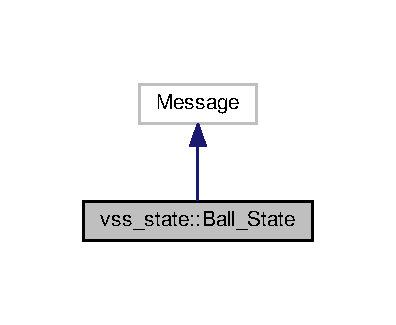
\includegraphics[width=190pt]{classvss__state_1_1Ball__State__inherit__graph}
\end{center}
\end{figure}


Diagrama de colaboração para vss\+\_\+state\+:\+:Ball\+\_\+\+State\+:\nopagebreak
\begin{figure}[H]
\begin{center}
\leavevmode
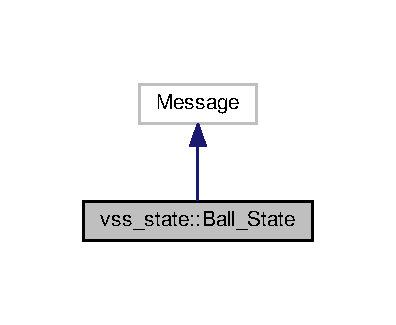
\includegraphics[width=190pt]{classvss__state_1_1Ball__State__coll__graph}
\end{center}
\end{figure}
\subsection*{Métodos Públicos}
\begin{DoxyCompactItemize}
\item 
{\bfseries Ball\+\_\+\+State} (const \hyperlink{classvss__state_1_1Ball__State}{Ball\+\_\+\+State} \&from)\hypertarget{classvss__state_1_1Ball__State_ac098b9cd5c2c3ddf8e51f0d2dbbf61fa}{}\label{classvss__state_1_1Ball__State_ac098b9cd5c2c3ddf8e51f0d2dbbf61fa}

\item 
\hyperlink{classvss__state_1_1Ball__State}{Ball\+\_\+\+State} \& {\bfseries operator=} (const \hyperlink{classvss__state_1_1Ball__State}{Ball\+\_\+\+State} \&from)\hypertarget{classvss__state_1_1Ball__State_aa6cd23990f9da364b87df28c633d5935}{}\label{classvss__state_1_1Ball__State_aa6cd23990f9da364b87df28c633d5935}

\item 
const \+::google\+::protobuf\+::\+Unknown\+Field\+Set \& {\bfseries unknown\+\_\+fields} () const \hypertarget{classvss__state_1_1Ball__State_a794e00572c1dadaee441bf94c11d7358}{}\label{classvss__state_1_1Ball__State_a794e00572c1dadaee441bf94c11d7358}

\item 
inline\+::google\+::protobuf\+::\+Unknown\+Field\+Set $\ast$ {\bfseries mutable\+\_\+unknown\+\_\+fields} ()\hypertarget{classvss__state_1_1Ball__State_a5d736fb563b0a4291d927a03394309b5}{}\label{classvss__state_1_1Ball__State_a5d736fb563b0a4291d927a03394309b5}

\item 
void {\bfseries Swap} (\hyperlink{classvss__state_1_1Ball__State}{Ball\+\_\+\+State} $\ast$other)\hypertarget{classvss__state_1_1Ball__State_a0e0face2c7b5e5b53793aa5e218a1623}{}\label{classvss__state_1_1Ball__State_a0e0face2c7b5e5b53793aa5e218a1623}

\item 
\hyperlink{classvss__state_1_1Ball__State}{Ball\+\_\+\+State} $\ast$ {\bfseries New} () const \hypertarget{classvss__state_1_1Ball__State_adc53dc3ec34e3721a215071717f7fde9}{}\label{classvss__state_1_1Ball__State_adc53dc3ec34e3721a215071717f7fde9}

\item 
\hyperlink{classvss__state_1_1Ball__State}{Ball\+\_\+\+State} $\ast$ {\bfseries New} (\+::google\+::protobuf\+::\+Arena $\ast$arena) const \hypertarget{classvss__state_1_1Ball__State_ac52ba5689a0c0f6361df46db91bdecf6}{}\label{classvss__state_1_1Ball__State_ac52ba5689a0c0f6361df46db91bdecf6}

\item 
void {\bfseries Copy\+From} (const \+::google\+::protobuf\+::\+Message \&from)\hypertarget{classvss__state_1_1Ball__State_a1b6e1fc62b0ed7f4a56f51107c2dea0c}{}\label{classvss__state_1_1Ball__State_a1b6e1fc62b0ed7f4a56f51107c2dea0c}

\item 
void {\bfseries Merge\+From} (const \+::google\+::protobuf\+::\+Message \&from)\hypertarget{classvss__state_1_1Ball__State_a23b0aa5fb0ead3fa0eb1d49f044a4108}{}\label{classvss__state_1_1Ball__State_a23b0aa5fb0ead3fa0eb1d49f044a4108}

\item 
void {\bfseries Copy\+From} (const \hyperlink{classvss__state_1_1Ball__State}{Ball\+\_\+\+State} \&from)\hypertarget{classvss__state_1_1Ball__State_abc6d9bde7cd19d33f5592fe7e89958f2}{}\label{classvss__state_1_1Ball__State_abc6d9bde7cd19d33f5592fe7e89958f2}

\item 
void {\bfseries Merge\+From} (const \hyperlink{classvss__state_1_1Ball__State}{Ball\+\_\+\+State} \&from)\hypertarget{classvss__state_1_1Ball__State_a6c0a4da68998dea51ba4971d3f3ae758}{}\label{classvss__state_1_1Ball__State_a6c0a4da68998dea51ba4971d3f3ae758}

\item 
void {\bfseries Clear} ()\hypertarget{classvss__state_1_1Ball__State_a23083679f69714534dff6d2fa4dfd69c}{}\label{classvss__state_1_1Ball__State_a23083679f69714534dff6d2fa4dfd69c}

\item 
bool {\bfseries Is\+Initialized} () const \hypertarget{classvss__state_1_1Ball__State_a86118bd22017a79d8bcecbb9759664ae}{}\label{classvss__state_1_1Ball__State_a86118bd22017a79d8bcecbb9759664ae}

\item 
int {\bfseries Byte\+Size} () const \hypertarget{classvss__state_1_1Ball__State_a37464e62ecce865fa9b7d71df18a6df2}{}\label{classvss__state_1_1Ball__State_a37464e62ecce865fa9b7d71df18a6df2}

\item 
bool {\bfseries Merge\+Partial\+From\+Coded\+Stream} (\+::google\+::protobuf\+::io\+::\+Coded\+Input\+Stream $\ast$input)\hypertarget{classvss__state_1_1Ball__State_a23384562e9b1779b7eae6df07fec8c08}{}\label{classvss__state_1_1Ball__State_a23384562e9b1779b7eae6df07fec8c08}

\item 
void {\bfseries Serialize\+With\+Cached\+Sizes} (\+::google\+::protobuf\+::io\+::\+Coded\+Output\+Stream $\ast$output) const \hypertarget{classvss__state_1_1Ball__State_ac9561ed1c347cc216c9adda156c8b1a7}{}\label{classvss__state_1_1Ball__State_ac9561ed1c347cc216c9adda156c8b1a7}

\item 
\+::google\+::protobuf\+::uint8 $\ast$ {\bfseries Internal\+Serialize\+With\+Cached\+Sizes\+To\+Array} (bool deterministic,\+::google\+::protobuf\+::uint8 $\ast$output) const \hypertarget{classvss__state_1_1Ball__State_ab4cba5d600b6ca3e6302ee7aaaa1c364}{}\label{classvss__state_1_1Ball__State_ab4cba5d600b6ca3e6302ee7aaaa1c364}

\item 
\+::google\+::protobuf\+::uint8 $\ast$ {\bfseries Serialize\+With\+Cached\+Sizes\+To\+Array} (\+::google\+::protobuf\+::uint8 $\ast$output) const \hypertarget{classvss__state_1_1Ball__State_a364e073f9074db05786bd455d88cdf6a}{}\label{classvss__state_1_1Ball__State_a364e073f9074db05786bd455d88cdf6a}

\item 
int {\bfseries Get\+Cached\+Size} () const \hypertarget{classvss__state_1_1Ball__State_a7f1be4451c61efb737a23f36191592f5}{}\label{classvss__state_1_1Ball__State_a7f1be4451c61efb737a23f36191592f5}

\item 
\+::google\+::protobuf\+::\+Metadata {\bfseries Get\+Metadata} () const \hypertarget{classvss__state_1_1Ball__State_ab93a553faefe3d3c98f56f6f84df0892}{}\label{classvss__state_1_1Ball__State_ab93a553faefe3d3c98f56f6f84df0892}

\item 
bool {\bfseries has\+\_\+pose} () const \hypertarget{classvss__state_1_1Ball__State_aeba993e45c63156eeb1b202c4e439559}{}\label{classvss__state_1_1Ball__State_aeba993e45c63156eeb1b202c4e439559}

\item 
void {\bfseries clear\+\_\+pose} ()\hypertarget{classvss__state_1_1Ball__State_aae55355551b9800c9a9f5b3b21fd6621}{}\label{classvss__state_1_1Ball__State_aae55355551b9800c9a9f5b3b21fd6621}

\item 
const \+::\hyperlink{classvss__state_1_1Pose}{vss\+\_\+state\+::\+Pose} \& {\bfseries pose} () const \hypertarget{classvss__state_1_1Ball__State_a2e0c721ce0540088e6015dcabc56c483}{}\label{classvss__state_1_1Ball__State_a2e0c721ce0540088e6015dcabc56c483}

\item 
\+::\hyperlink{classvss__state_1_1Pose}{vss\+\_\+state\+::\+Pose} $\ast$ {\bfseries mutable\+\_\+pose} ()\hypertarget{classvss__state_1_1Ball__State_a4c639ae56018c9b8bb3bd857565b9151}{}\label{classvss__state_1_1Ball__State_a4c639ae56018c9b8bb3bd857565b9151}

\item 
\+::\hyperlink{classvss__state_1_1Pose}{vss\+\_\+state\+::\+Pose} $\ast$ {\bfseries release\+\_\+pose} ()\hypertarget{classvss__state_1_1Ball__State_a9a5aa9e491a204a03a7c50455e455892}{}\label{classvss__state_1_1Ball__State_a9a5aa9e491a204a03a7c50455e455892}

\item 
void {\bfseries set\+\_\+allocated\+\_\+pose} (\+::\hyperlink{classvss__state_1_1Pose}{vss\+\_\+state\+::\+Pose} $\ast$pose)\hypertarget{classvss__state_1_1Ball__State_a2bf1fa45ff9a17edf9116a5422fafc43}{}\label{classvss__state_1_1Ball__State_a2bf1fa45ff9a17edf9116a5422fafc43}

\item 
bool {\bfseries has\+\_\+v\+\_\+pose} () const \hypertarget{classvss__state_1_1Ball__State_a07ae64c42cc9e02e4dfbac72ffebf930}{}\label{classvss__state_1_1Ball__State_a07ae64c42cc9e02e4dfbac72ffebf930}

\item 
void {\bfseries clear\+\_\+v\+\_\+pose} ()\hypertarget{classvss__state_1_1Ball__State_a9ba97738218066dbf5ec163a0d5470ad}{}\label{classvss__state_1_1Ball__State_a9ba97738218066dbf5ec163a0d5470ad}

\item 
const \+::\hyperlink{classvss__state_1_1Pose}{vss\+\_\+state\+::\+Pose} \& {\bfseries v\+\_\+pose} () const \hypertarget{classvss__state_1_1Ball__State_a96bd044402758e810a78fd2a1e2a9c0c}{}\label{classvss__state_1_1Ball__State_a96bd044402758e810a78fd2a1e2a9c0c}

\item 
\+::\hyperlink{classvss__state_1_1Pose}{vss\+\_\+state\+::\+Pose} $\ast$ {\bfseries mutable\+\_\+v\+\_\+pose} ()\hypertarget{classvss__state_1_1Ball__State_a13b650e7cc6d2b306eb072522922df06}{}\label{classvss__state_1_1Ball__State_a13b650e7cc6d2b306eb072522922df06}

\item 
\+::\hyperlink{classvss__state_1_1Pose}{vss\+\_\+state\+::\+Pose} $\ast$ {\bfseries release\+\_\+v\+\_\+pose} ()\hypertarget{classvss__state_1_1Ball__State_a56eb1c3147c39d721705f2ebeb825e8b}{}\label{classvss__state_1_1Ball__State_a56eb1c3147c39d721705f2ebeb825e8b}

\item 
void {\bfseries set\+\_\+allocated\+\_\+v\+\_\+pose} (\+::\hyperlink{classvss__state_1_1Pose}{vss\+\_\+state\+::\+Pose} $\ast$v\+\_\+pose)\hypertarget{classvss__state_1_1Ball__State_aae94edb5b999518e21d7681a49a3ec50}{}\label{classvss__state_1_1Ball__State_aae94edb5b999518e21d7681a49a3ec50}

\item 
bool {\bfseries has\+\_\+k\+\_\+pose} () const \hypertarget{classvss__state_1_1Ball__State_ad7e1b1d6aa0f6fb49c219a6477c4d415}{}\label{classvss__state_1_1Ball__State_ad7e1b1d6aa0f6fb49c219a6477c4d415}

\item 
void {\bfseries clear\+\_\+k\+\_\+pose} ()\hypertarget{classvss__state_1_1Ball__State_ae093f7fcee14bf36d481defd042531a2}{}\label{classvss__state_1_1Ball__State_ae093f7fcee14bf36d481defd042531a2}

\item 
const \+::\hyperlink{classvss__state_1_1Pose}{vss\+\_\+state\+::\+Pose} \& {\bfseries k\+\_\+pose} () const \hypertarget{classvss__state_1_1Ball__State_ad50969e1c0311df60af86339531e95f4}{}\label{classvss__state_1_1Ball__State_ad50969e1c0311df60af86339531e95f4}

\item 
\+::\hyperlink{classvss__state_1_1Pose}{vss\+\_\+state\+::\+Pose} $\ast$ {\bfseries mutable\+\_\+k\+\_\+pose} ()\hypertarget{classvss__state_1_1Ball__State_a3953797cd45c0dc2ad6bc73c3effce62}{}\label{classvss__state_1_1Ball__State_a3953797cd45c0dc2ad6bc73c3effce62}

\item 
\+::\hyperlink{classvss__state_1_1Pose}{vss\+\_\+state\+::\+Pose} $\ast$ {\bfseries release\+\_\+k\+\_\+pose} ()\hypertarget{classvss__state_1_1Ball__State_a1ee5fc6190261a2b39a059ea215c0393}{}\label{classvss__state_1_1Ball__State_a1ee5fc6190261a2b39a059ea215c0393}

\item 
void {\bfseries set\+\_\+allocated\+\_\+k\+\_\+pose} (\+::\hyperlink{classvss__state_1_1Pose}{vss\+\_\+state\+::\+Pose} $\ast$k\+\_\+pose)\hypertarget{classvss__state_1_1Ball__State_ae45eb76e5900376f40deaeaf0efbac2d}{}\label{classvss__state_1_1Ball__State_ae45eb76e5900376f40deaeaf0efbac2d}

\item 
bool {\bfseries has\+\_\+k\+\_\+v\+\_\+pose} () const \hypertarget{classvss__state_1_1Ball__State_a930e42deca924b95399f2bfd616cfbe5}{}\label{classvss__state_1_1Ball__State_a930e42deca924b95399f2bfd616cfbe5}

\item 
void {\bfseries clear\+\_\+k\+\_\+v\+\_\+pose} ()\hypertarget{classvss__state_1_1Ball__State_a8bb6d21c1aad5ec994362b48b42eb31d}{}\label{classvss__state_1_1Ball__State_a8bb6d21c1aad5ec994362b48b42eb31d}

\item 
const \+::\hyperlink{classvss__state_1_1Pose}{vss\+\_\+state\+::\+Pose} \& {\bfseries k\+\_\+v\+\_\+pose} () const \hypertarget{classvss__state_1_1Ball__State_a145febfeefee751422babd01a98a2c8b}{}\label{classvss__state_1_1Ball__State_a145febfeefee751422babd01a98a2c8b}

\item 
\+::\hyperlink{classvss__state_1_1Pose}{vss\+\_\+state\+::\+Pose} $\ast$ {\bfseries mutable\+\_\+k\+\_\+v\+\_\+pose} ()\hypertarget{classvss__state_1_1Ball__State_ac3b62e9cfb792bc6942a98fb9aceb5ff}{}\label{classvss__state_1_1Ball__State_ac3b62e9cfb792bc6942a98fb9aceb5ff}

\item 
\+::\hyperlink{classvss__state_1_1Pose}{vss\+\_\+state\+::\+Pose} $\ast$ {\bfseries release\+\_\+k\+\_\+v\+\_\+pose} ()\hypertarget{classvss__state_1_1Ball__State_a2245ebd735cebe20ca68a202a8a0adf3}{}\label{classvss__state_1_1Ball__State_a2245ebd735cebe20ca68a202a8a0adf3}

\item 
void {\bfseries set\+\_\+allocated\+\_\+k\+\_\+v\+\_\+pose} (\+::\hyperlink{classvss__state_1_1Pose}{vss\+\_\+state\+::\+Pose} $\ast$k\+\_\+v\+\_\+pose)\hypertarget{classvss__state_1_1Ball__State_a191d7bdd20328826d877b1219da91e3e}{}\label{classvss__state_1_1Ball__State_a191d7bdd20328826d877b1219da91e3e}

\end{DoxyCompactItemize}
\subsection*{Métodos Públicos Estáticos}
\begin{DoxyCompactItemize}
\item 
static const \+::google\+::protobuf\+::\+Descriptor $\ast$ {\bfseries descriptor} ()\hypertarget{classvss__state_1_1Ball__State_adfc29a0088d19129c759d22494a74443}{}\label{classvss__state_1_1Ball__State_adfc29a0088d19129c759d22494a74443}

\item 
static const \hyperlink{classvss__state_1_1Ball__State}{Ball\+\_\+\+State} \& {\bfseries default\+\_\+instance} ()\hypertarget{classvss__state_1_1Ball__State_a762be08a3ad7dcbec17beb380b860f95}{}\label{classvss__state_1_1Ball__State_a762be08a3ad7dcbec17beb380b860f95}

\end{DoxyCompactItemize}
\subsection*{Atributos Estáticos Públicos}
\begin{DoxyCompactItemize}
\item 
static const int {\bfseries k\+Pose\+Field\+Number} = 1\hypertarget{classvss__state_1_1Ball__State_aa0d51eebda087326095eff02cc80481c}{}\label{classvss__state_1_1Ball__State_aa0d51eebda087326095eff02cc80481c}

\item 
static const int {\bfseries k\+V\+Pose\+Field\+Number} = 2\hypertarget{classvss__state_1_1Ball__State_aa9df3d7a047296c119dfc35ae5e86b54}{}\label{classvss__state_1_1Ball__State_aa9df3d7a047296c119dfc35ae5e86b54}

\item 
static const int {\bfseries k\+K\+Pose\+Field\+Number} = 3\hypertarget{classvss__state_1_1Ball__State_a31603cacf64917d3088585f33290114a}{}\label{classvss__state_1_1Ball__State_a31603cacf64917d3088585f33290114a}

\item 
static const int {\bfseries k\+K\+V\+Pose\+Field\+Number} = 4\hypertarget{classvss__state_1_1Ball__State_a8d49de5cec51b6a22e828da61fa8810b}{}\label{classvss__state_1_1Ball__State_a8d49de5cec51b6a22e828da61fa8810b}

\end{DoxyCompactItemize}
\subsection*{Amigas}
\begin{DoxyCompactItemize}
\item 
void {\bfseries protobuf\+\_\+\+Add\+Desc\+\_\+state\+\_\+2eproto} ()\hypertarget{classvss__state_1_1Ball__State_aab1a2c258f8122a403a979ff57e2a706}{}\label{classvss__state_1_1Ball__State_aab1a2c258f8122a403a979ff57e2a706}

\item 
void {\bfseries protobuf\+\_\+\+Assign\+Desc\+\_\+state\+\_\+2eproto} ()\hypertarget{classvss__state_1_1Ball__State_a57d9367bc8a7a94ead11d11194cca1b6}{}\label{classvss__state_1_1Ball__State_a57d9367bc8a7a94ead11d11194cca1b6}

\item 
void {\bfseries protobuf\+\_\+\+Shutdown\+File\+\_\+state\+\_\+2eproto} ()\hypertarget{classvss__state_1_1Ball__State_a4e6dc5e8e72799859c4e9556d090e57d}{}\label{classvss__state_1_1Ball__State_a4e6dc5e8e72799859c4e9556d090e57d}

\end{DoxyCompactItemize}


A documentação para esta classe foi gerada a partir dos seguintes arquivos\+:\begin{DoxyCompactItemize}
\item 
/home/johnathan/\+Repositories/\+S\+I\+R\+Lab/\+Projects/\+V\+S\+S-\/\+Viewer/src/\+V\+S\+S-\/\+Interface/protos/state.\+pb.\+h\item 
/home/johnathan/\+Repositories/\+S\+I\+R\+Lab/\+Projects/\+V\+S\+S-\/\+Viewer/src/\+V\+S\+S-\/\+Interface/protos/state.\+pb.\+cc\end{DoxyCompactItemize}

\hypertarget{classvss__command_1_1Global__Commands}{}\section{Referência da Classe vss\+\_\+command\+:\+:Global\+\_\+\+Commands}
\label{classvss__command_1_1Global__Commands}\index{vss\+\_\+command\+::\+Global\+\_\+\+Commands@{vss\+\_\+command\+::\+Global\+\_\+\+Commands}}


Diagrama de Hierarquia para vss\+\_\+command\+:\+:Global\+\_\+\+Commands\+:\nopagebreak
\begin{figure}[H]
\begin{center}
\leavevmode
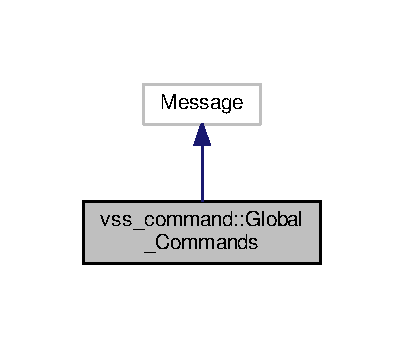
\includegraphics[width=194pt]{classvss__command_1_1Global__Commands__inherit__graph}
\end{center}
\end{figure}


Diagrama de colaboração para vss\+\_\+command\+:\+:Global\+\_\+\+Commands\+:\nopagebreak
\begin{figure}[H]
\begin{center}
\leavevmode
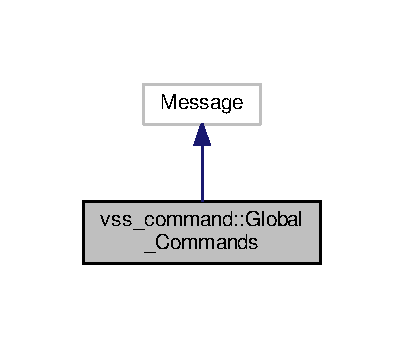
\includegraphics[width=194pt]{classvss__command_1_1Global__Commands__coll__graph}
\end{center}
\end{figure}
\subsection*{Métodos Públicos}
\begin{DoxyCompactItemize}
\item 
{\bfseries Global\+\_\+\+Commands} (const \hyperlink{classvss__command_1_1Global__Commands}{Global\+\_\+\+Commands} \&from)\hypertarget{classvss__command_1_1Global__Commands_ac5a1e52df1880363fccb681c303ec821}{}\label{classvss__command_1_1Global__Commands_ac5a1e52df1880363fccb681c303ec821}

\item 
\hyperlink{classvss__command_1_1Global__Commands}{Global\+\_\+\+Commands} \& {\bfseries operator=} (const \hyperlink{classvss__command_1_1Global__Commands}{Global\+\_\+\+Commands} \&from)\hypertarget{classvss__command_1_1Global__Commands_a1e2590dfc4b0e2c8c20a8f5c68531a22}{}\label{classvss__command_1_1Global__Commands_a1e2590dfc4b0e2c8c20a8f5c68531a22}

\item 
const \+::google\+::protobuf\+::\+Unknown\+Field\+Set \& {\bfseries unknown\+\_\+fields} () const \hypertarget{classvss__command_1_1Global__Commands_aadc4690c81ad4df3443b087428e1de73}{}\label{classvss__command_1_1Global__Commands_aadc4690c81ad4df3443b087428e1de73}

\item 
inline\+::google\+::protobuf\+::\+Unknown\+Field\+Set $\ast$ {\bfseries mutable\+\_\+unknown\+\_\+fields} ()\hypertarget{classvss__command_1_1Global__Commands_a1882397164e8072272d76b8172991013}{}\label{classvss__command_1_1Global__Commands_a1882397164e8072272d76b8172991013}

\item 
void {\bfseries Swap} (\hyperlink{classvss__command_1_1Global__Commands}{Global\+\_\+\+Commands} $\ast$other)\hypertarget{classvss__command_1_1Global__Commands_a1bf67bb767a2b899fceb94bf88a52ba7}{}\label{classvss__command_1_1Global__Commands_a1bf67bb767a2b899fceb94bf88a52ba7}

\item 
\hyperlink{classvss__command_1_1Global__Commands}{Global\+\_\+\+Commands} $\ast$ {\bfseries New} () const \hypertarget{classvss__command_1_1Global__Commands_ae7247bd1baff094512d36f88c3abc1ad}{}\label{classvss__command_1_1Global__Commands_ae7247bd1baff094512d36f88c3abc1ad}

\item 
\hyperlink{classvss__command_1_1Global__Commands}{Global\+\_\+\+Commands} $\ast$ {\bfseries New} (\+::google\+::protobuf\+::\+Arena $\ast$arena) const \hypertarget{classvss__command_1_1Global__Commands_a8dfab8af897b1445455e06ac02ebaac0}{}\label{classvss__command_1_1Global__Commands_a8dfab8af897b1445455e06ac02ebaac0}

\item 
void {\bfseries Copy\+From} (const \+::google\+::protobuf\+::\+Message \&from)\hypertarget{classvss__command_1_1Global__Commands_a4bd5bb12d6e5f08346704aa04a30fe57}{}\label{classvss__command_1_1Global__Commands_a4bd5bb12d6e5f08346704aa04a30fe57}

\item 
void {\bfseries Merge\+From} (const \+::google\+::protobuf\+::\+Message \&from)\hypertarget{classvss__command_1_1Global__Commands_a70b24974df993bc6cd742f074555544b}{}\label{classvss__command_1_1Global__Commands_a70b24974df993bc6cd742f074555544b}

\item 
void {\bfseries Copy\+From} (const \hyperlink{classvss__command_1_1Global__Commands}{Global\+\_\+\+Commands} \&from)\hypertarget{classvss__command_1_1Global__Commands_a2c2be618a14de139a996c3f40cdcaa7c}{}\label{classvss__command_1_1Global__Commands_a2c2be618a14de139a996c3f40cdcaa7c}

\item 
void {\bfseries Merge\+From} (const \hyperlink{classvss__command_1_1Global__Commands}{Global\+\_\+\+Commands} \&from)\hypertarget{classvss__command_1_1Global__Commands_a72522cd185ed392c8dba2b746f1c10be}{}\label{classvss__command_1_1Global__Commands_a72522cd185ed392c8dba2b746f1c10be}

\item 
void {\bfseries Clear} ()\hypertarget{classvss__command_1_1Global__Commands_a9027fa1a333a49d2a9e7927f1241d2d7}{}\label{classvss__command_1_1Global__Commands_a9027fa1a333a49d2a9e7927f1241d2d7}

\item 
bool {\bfseries Is\+Initialized} () const \hypertarget{classvss__command_1_1Global__Commands_ab59f63095dd243cd7311d9142a9326ef}{}\label{classvss__command_1_1Global__Commands_ab59f63095dd243cd7311d9142a9326ef}

\item 
int {\bfseries Byte\+Size} () const \hypertarget{classvss__command_1_1Global__Commands_a05036b0569ebf9d13ff9cee1430ffb12}{}\label{classvss__command_1_1Global__Commands_a05036b0569ebf9d13ff9cee1430ffb12}

\item 
bool {\bfseries Merge\+Partial\+From\+Coded\+Stream} (\+::google\+::protobuf\+::io\+::\+Coded\+Input\+Stream $\ast$input)\hypertarget{classvss__command_1_1Global__Commands_a0d0fcd0747bad0226fb5a0829f45ed1b}{}\label{classvss__command_1_1Global__Commands_a0d0fcd0747bad0226fb5a0829f45ed1b}

\item 
void {\bfseries Serialize\+With\+Cached\+Sizes} (\+::google\+::protobuf\+::io\+::\+Coded\+Output\+Stream $\ast$output) const \hypertarget{classvss__command_1_1Global__Commands_a35292dbb1e0ac73f11bedc01a64e751e}{}\label{classvss__command_1_1Global__Commands_a35292dbb1e0ac73f11bedc01a64e751e}

\item 
\+::google\+::protobuf\+::uint8 $\ast$ {\bfseries Internal\+Serialize\+With\+Cached\+Sizes\+To\+Array} (bool deterministic,\+::google\+::protobuf\+::uint8 $\ast$output) const \hypertarget{classvss__command_1_1Global__Commands_a68d33135851d0d816141df590ddf789a}{}\label{classvss__command_1_1Global__Commands_a68d33135851d0d816141df590ddf789a}

\item 
\+::google\+::protobuf\+::uint8 $\ast$ {\bfseries Serialize\+With\+Cached\+Sizes\+To\+Array} (\+::google\+::protobuf\+::uint8 $\ast$output) const \hypertarget{classvss__command_1_1Global__Commands_a410002d27fea7d706ebf87bbf1fb74c5}{}\label{classvss__command_1_1Global__Commands_a410002d27fea7d706ebf87bbf1fb74c5}

\item 
int {\bfseries Get\+Cached\+Size} () const \hypertarget{classvss__command_1_1Global__Commands_a87d23baa19f2c0272a75e15dfa234f08}{}\label{classvss__command_1_1Global__Commands_a87d23baa19f2c0272a75e15dfa234f08}

\item 
\+::google\+::protobuf\+::\+Metadata {\bfseries Get\+Metadata} () const \hypertarget{classvss__command_1_1Global__Commands_ae82e1f8fbfdf6f364c915da6d0e12f33}{}\label{classvss__command_1_1Global__Commands_ae82e1f8fbfdf6f364c915da6d0e12f33}

\item 
bool {\bfseries has\+\_\+id} () const \hypertarget{classvss__command_1_1Global__Commands_a70a923cca7611e0bd3c322a1ac5e91ba}{}\label{classvss__command_1_1Global__Commands_a70a923cca7611e0bd3c322a1ac5e91ba}

\item 
void {\bfseries clear\+\_\+id} ()\hypertarget{classvss__command_1_1Global__Commands_a32c51afe77b984a2be61e786893dd382}{}\label{classvss__command_1_1Global__Commands_a32c51afe77b984a2be61e786893dd382}

\item 
\+::google\+::protobuf\+::uint32 {\bfseries id} () const \hypertarget{classvss__command_1_1Global__Commands_ac4b50f174ae21e1ef747b8d2498d9651}{}\label{classvss__command_1_1Global__Commands_ac4b50f174ae21e1ef747b8d2498d9651}

\item 
void {\bfseries set\+\_\+id} (\+::google\+::protobuf\+::uint32 value)\hypertarget{classvss__command_1_1Global__Commands_aba49ba26507d3a54403584352f3dde90}{}\label{classvss__command_1_1Global__Commands_aba49ba26507d3a54403584352f3dde90}

\item 
bool {\bfseries has\+\_\+is\+\_\+team\+\_\+yellow} () const \hypertarget{classvss__command_1_1Global__Commands_a01e1a3bf6986a61900153eec4e51ac9b}{}\label{classvss__command_1_1Global__Commands_a01e1a3bf6986a61900153eec4e51ac9b}

\item 
void {\bfseries clear\+\_\+is\+\_\+team\+\_\+yellow} ()\hypertarget{classvss__command_1_1Global__Commands_ad626702bff23b842c6c342fb94ed9097}{}\label{classvss__command_1_1Global__Commands_ad626702bff23b842c6c342fb94ed9097}

\item 
bool {\bfseries is\+\_\+team\+\_\+yellow} () const \hypertarget{classvss__command_1_1Global__Commands_a82e8f2fd24d0bcbf30e924d18dd8bba8}{}\label{classvss__command_1_1Global__Commands_a82e8f2fd24d0bcbf30e924d18dd8bba8}

\item 
void {\bfseries set\+\_\+is\+\_\+team\+\_\+yellow} (bool value)\hypertarget{classvss__command_1_1Global__Commands_ac7855fe013be0c1be3f573a1b6eb47dc}{}\label{classvss__command_1_1Global__Commands_ac7855fe013be0c1be3f573a1b6eb47dc}

\item 
int {\bfseries robot\+\_\+commands\+\_\+size} () const \hypertarget{classvss__command_1_1Global__Commands_a09f12589e89e8d27a0e0d6fb7ecbcee3}{}\label{classvss__command_1_1Global__Commands_a09f12589e89e8d27a0e0d6fb7ecbcee3}

\item 
void {\bfseries clear\+\_\+robot\+\_\+commands} ()\hypertarget{classvss__command_1_1Global__Commands_a2624ae56ed92fe0cf6617f8c740ad2d2}{}\label{classvss__command_1_1Global__Commands_a2624ae56ed92fe0cf6617f8c740ad2d2}

\item 
const \+::\hyperlink{classvss__command_1_1Robot__Command}{vss\+\_\+command\+::\+Robot\+\_\+\+Command} \& {\bfseries robot\+\_\+commands} (int index) const \hypertarget{classvss__command_1_1Global__Commands_aa6bd99500ef874f4a68cbf1adecf0fd1}{}\label{classvss__command_1_1Global__Commands_aa6bd99500ef874f4a68cbf1adecf0fd1}

\item 
\+::\hyperlink{classvss__command_1_1Robot__Command}{vss\+\_\+command\+::\+Robot\+\_\+\+Command} $\ast$ {\bfseries mutable\+\_\+robot\+\_\+commands} (int index)\hypertarget{classvss__command_1_1Global__Commands_a08dc88b20105318b2cc8bbbbf2300581}{}\label{classvss__command_1_1Global__Commands_a08dc88b20105318b2cc8bbbbf2300581}

\item 
\+::\hyperlink{classvss__command_1_1Robot__Command}{vss\+\_\+command\+::\+Robot\+\_\+\+Command} $\ast$ {\bfseries add\+\_\+robot\+\_\+commands} ()\hypertarget{classvss__command_1_1Global__Commands_add6abc22ca67ffa146cfba3e0b17ad2b}{}\label{classvss__command_1_1Global__Commands_add6abc22ca67ffa146cfba3e0b17ad2b}

\item 
\+::google\+::protobuf\+::\+Repeated\+Ptr\+Field$<$ \+::\hyperlink{classvss__command_1_1Robot__Command}{vss\+\_\+command\+::\+Robot\+\_\+\+Command} $>$ $\ast$ {\bfseries mutable\+\_\+robot\+\_\+commands} ()\hypertarget{classvss__command_1_1Global__Commands_a3de88f16ed28f63fed38eff2ef169df4}{}\label{classvss__command_1_1Global__Commands_a3de88f16ed28f63fed38eff2ef169df4}

\item 
const \+::google\+::protobuf\+::\+Repeated\+Ptr\+Field$<$ \+::\hyperlink{classvss__command_1_1Robot__Command}{vss\+\_\+command\+::\+Robot\+\_\+\+Command} $>$ \& {\bfseries robot\+\_\+commands} () const \hypertarget{classvss__command_1_1Global__Commands_acb14464615fbad56ce9a1da3ce46373a}{}\label{classvss__command_1_1Global__Commands_acb14464615fbad56ce9a1da3ce46373a}

\item 
bool {\bfseries has\+\_\+situation} () const \hypertarget{classvss__command_1_1Global__Commands_a8ef03dbd77af5f6170759b71949c50c2}{}\label{classvss__command_1_1Global__Commands_a8ef03dbd77af5f6170759b71949c50c2}

\item 
void {\bfseries clear\+\_\+situation} ()\hypertarget{classvss__command_1_1Global__Commands_a7117b4a642bd8d833e6a431073efc94d}{}\label{classvss__command_1_1Global__Commands_a7117b4a642bd8d833e6a431073efc94d}

\item 
\+::google\+::protobuf\+::uint32 {\bfseries situation} () const \hypertarget{classvss__command_1_1Global__Commands_a712002b02d4d401a76479434fd97dc17}{}\label{classvss__command_1_1Global__Commands_a712002b02d4d401a76479434fd97dc17}

\item 
void {\bfseries set\+\_\+situation} (\+::google\+::protobuf\+::uint32 value)\hypertarget{classvss__command_1_1Global__Commands_a8d96bc1eeac62f3e318c258bfea74258}{}\label{classvss__command_1_1Global__Commands_a8d96bc1eeac62f3e318c258bfea74258}

\end{DoxyCompactItemize}
\subsection*{Métodos Públicos Estáticos}
\begin{DoxyCompactItemize}
\item 
static const \+::google\+::protobuf\+::\+Descriptor $\ast$ {\bfseries descriptor} ()\hypertarget{classvss__command_1_1Global__Commands_a26e4245a80fa599d0e30613122af7ad9}{}\label{classvss__command_1_1Global__Commands_a26e4245a80fa599d0e30613122af7ad9}

\item 
static const \hyperlink{classvss__command_1_1Global__Commands}{Global\+\_\+\+Commands} \& {\bfseries default\+\_\+instance} ()\hypertarget{classvss__command_1_1Global__Commands_a9e44db388aae4a529e0bff71979eea66}{}\label{classvss__command_1_1Global__Commands_a9e44db388aae4a529e0bff71979eea66}

\end{DoxyCompactItemize}
\subsection*{Atributos Estáticos Públicos}
\begin{DoxyCompactItemize}
\item 
static const int {\bfseries k\+Id\+Field\+Number} = 1\hypertarget{classvss__command_1_1Global__Commands_a67c9ce208f0648844211d1faca128e34}{}\label{classvss__command_1_1Global__Commands_a67c9ce208f0648844211d1faca128e34}

\item 
static const int {\bfseries k\+Is\+Team\+Yellow\+Field\+Number} = 2\hypertarget{classvss__command_1_1Global__Commands_a90443d587b7a5171b061ec96660b04ef}{}\label{classvss__command_1_1Global__Commands_a90443d587b7a5171b061ec96660b04ef}

\item 
static const int {\bfseries k\+Robot\+Commands\+Field\+Number} = 3\hypertarget{classvss__command_1_1Global__Commands_a65b203ec091ad5cce5fcb7b34b01bcf1}{}\label{classvss__command_1_1Global__Commands_a65b203ec091ad5cce5fcb7b34b01bcf1}

\item 
static const int {\bfseries k\+Situation\+Field\+Number} = 4\hypertarget{classvss__command_1_1Global__Commands_a98597b870f4ed51cf1b516211e3f785d}{}\label{classvss__command_1_1Global__Commands_a98597b870f4ed51cf1b516211e3f785d}

\end{DoxyCompactItemize}
\subsection*{Amigas}
\begin{DoxyCompactItemize}
\item 
void {\bfseries protobuf\+\_\+\+Add\+Desc\+\_\+command\+\_\+2eproto} ()\hypertarget{classvss__command_1_1Global__Commands_a4825d92f856fcb4b02c67b601c433796}{}\label{classvss__command_1_1Global__Commands_a4825d92f856fcb4b02c67b601c433796}

\item 
void {\bfseries protobuf\+\_\+\+Assign\+Desc\+\_\+command\+\_\+2eproto} ()\hypertarget{classvss__command_1_1Global__Commands_a4c6fb97c25079d49daf010087d869100}{}\label{classvss__command_1_1Global__Commands_a4c6fb97c25079d49daf010087d869100}

\item 
void {\bfseries protobuf\+\_\+\+Shutdown\+File\+\_\+command\+\_\+2eproto} ()\hypertarget{classvss__command_1_1Global__Commands_a4cf10633ad46690f5eec6bdbbcf62de0}{}\label{classvss__command_1_1Global__Commands_a4cf10633ad46690f5eec6bdbbcf62de0}

\end{DoxyCompactItemize}


A documentação para esta classe foi gerada a partir dos seguintes arquivos\+:\begin{DoxyCompactItemize}
\item 
/home/johnathan/\+Repositories/\+S\+I\+R\+Lab/\+Public/\+V\+S\+S-\/\+Viewer/src/\+V\+S\+S-\/\+Interface/protos/command.\+pb.\+h\item 
/home/johnathan/\+Repositories/\+S\+I\+R\+Lab/\+Public/\+V\+S\+S-\/\+Viewer/src/\+V\+S\+S-\/\+Interface/protos/command.\+pb.\+cc\end{DoxyCompactItemize}

\hypertarget{classvss__debug_1_1Global__Debug}{}\section{Referência da Classe vss\+\_\+debug\+:\+:Global\+\_\+\+Debug}
\label{classvss__debug_1_1Global__Debug}\index{vss\+\_\+debug\+::\+Global\+\_\+\+Debug@{vss\+\_\+debug\+::\+Global\+\_\+\+Debug}}


Diagrama de Hierarquia para vss\+\_\+debug\+:\+:Global\+\_\+\+Debug\+:\nopagebreak
\begin{figure}[H]
\begin{center}
\leavevmode
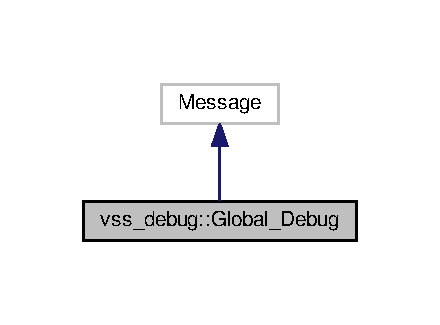
\includegraphics[width=211pt]{classvss__debug_1_1Global__Debug__inherit__graph}
\end{center}
\end{figure}


Diagrama de colaboração para vss\+\_\+debug\+:\+:Global\+\_\+\+Debug\+:\nopagebreak
\begin{figure}[H]
\begin{center}
\leavevmode
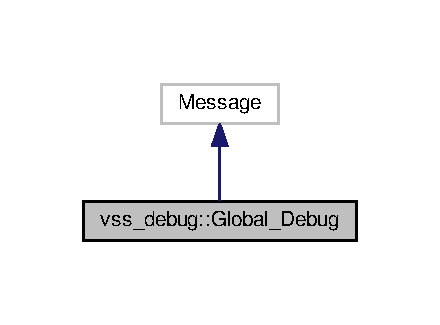
\includegraphics[width=211pt]{classvss__debug_1_1Global__Debug__coll__graph}
\end{center}
\end{figure}
\subsection*{Métodos Públicos}
\begin{DoxyCompactItemize}
\item 
{\bfseries Global\+\_\+\+Debug} (const \hyperlink{classvss__debug_1_1Global__Debug}{Global\+\_\+\+Debug} \&from)\hypertarget{classvss__debug_1_1Global__Debug_a3c59c9a4d51b615ed334ec247115bdc7}{}\label{classvss__debug_1_1Global__Debug_a3c59c9a4d51b615ed334ec247115bdc7}

\item 
\hyperlink{classvss__debug_1_1Global__Debug}{Global\+\_\+\+Debug} \& {\bfseries operator=} (const \hyperlink{classvss__debug_1_1Global__Debug}{Global\+\_\+\+Debug} \&from)\hypertarget{classvss__debug_1_1Global__Debug_a12877416f81456cec9814821b64da40c}{}\label{classvss__debug_1_1Global__Debug_a12877416f81456cec9814821b64da40c}

\item 
const \+::google\+::protobuf\+::\+Unknown\+Field\+Set \& {\bfseries unknown\+\_\+fields} () const \hypertarget{classvss__debug_1_1Global__Debug_a168d0c1a65d08db337ecedce80265660}{}\label{classvss__debug_1_1Global__Debug_a168d0c1a65d08db337ecedce80265660}

\item 
inline\+::google\+::protobuf\+::\+Unknown\+Field\+Set $\ast$ {\bfseries mutable\+\_\+unknown\+\_\+fields} ()\hypertarget{classvss__debug_1_1Global__Debug_a6fd5cc3c20a7cfa3f956285d73657ac3}{}\label{classvss__debug_1_1Global__Debug_a6fd5cc3c20a7cfa3f956285d73657ac3}

\item 
void {\bfseries Swap} (\hyperlink{classvss__debug_1_1Global__Debug}{Global\+\_\+\+Debug} $\ast$other)\hypertarget{classvss__debug_1_1Global__Debug_a86a35c7744c5f052407ea724cba349ca}{}\label{classvss__debug_1_1Global__Debug_a86a35c7744c5f052407ea724cba349ca}

\item 
\hyperlink{classvss__debug_1_1Global__Debug}{Global\+\_\+\+Debug} $\ast$ {\bfseries New} () const \hypertarget{classvss__debug_1_1Global__Debug_a4cec6538e5e848660550c88bd5df8f56}{}\label{classvss__debug_1_1Global__Debug_a4cec6538e5e848660550c88bd5df8f56}

\item 
\hyperlink{classvss__debug_1_1Global__Debug}{Global\+\_\+\+Debug} $\ast$ {\bfseries New} (\+::google\+::protobuf\+::\+Arena $\ast$arena) const \hypertarget{classvss__debug_1_1Global__Debug_a82c5f551838b587f155b3249007fced0}{}\label{classvss__debug_1_1Global__Debug_a82c5f551838b587f155b3249007fced0}

\item 
void {\bfseries Copy\+From} (const \+::google\+::protobuf\+::\+Message \&from)\hypertarget{classvss__debug_1_1Global__Debug_a77f2c60180607e1cfc605fdcb913a79b}{}\label{classvss__debug_1_1Global__Debug_a77f2c60180607e1cfc605fdcb913a79b}

\item 
void {\bfseries Merge\+From} (const \+::google\+::protobuf\+::\+Message \&from)\hypertarget{classvss__debug_1_1Global__Debug_ac69a78aa769aa584c765ecceaf7fba5b}{}\label{classvss__debug_1_1Global__Debug_ac69a78aa769aa584c765ecceaf7fba5b}

\item 
void {\bfseries Copy\+From} (const \hyperlink{classvss__debug_1_1Global__Debug}{Global\+\_\+\+Debug} \&from)\hypertarget{classvss__debug_1_1Global__Debug_a090fc098850d32138d9b638bc0efe457}{}\label{classvss__debug_1_1Global__Debug_a090fc098850d32138d9b638bc0efe457}

\item 
void {\bfseries Merge\+From} (const \hyperlink{classvss__debug_1_1Global__Debug}{Global\+\_\+\+Debug} \&from)\hypertarget{classvss__debug_1_1Global__Debug_acef49d0fd298c356e6c11fd1c3407681}{}\label{classvss__debug_1_1Global__Debug_acef49d0fd298c356e6c11fd1c3407681}

\item 
void {\bfseries Clear} ()\hypertarget{classvss__debug_1_1Global__Debug_a903e3d4e444632048f78d7c2e707367b}{}\label{classvss__debug_1_1Global__Debug_a903e3d4e444632048f78d7c2e707367b}

\item 
bool {\bfseries Is\+Initialized} () const \hypertarget{classvss__debug_1_1Global__Debug_accd80d5e07db4a5cf2e2f254f500b874}{}\label{classvss__debug_1_1Global__Debug_accd80d5e07db4a5cf2e2f254f500b874}

\item 
int {\bfseries Byte\+Size} () const \hypertarget{classvss__debug_1_1Global__Debug_ada6ae1d20ee44cb870fe5175a371dc43}{}\label{classvss__debug_1_1Global__Debug_ada6ae1d20ee44cb870fe5175a371dc43}

\item 
bool {\bfseries Merge\+Partial\+From\+Coded\+Stream} (\+::google\+::protobuf\+::io\+::\+Coded\+Input\+Stream $\ast$input)\hypertarget{classvss__debug_1_1Global__Debug_a75302270b4981afeda6355bcda846f24}{}\label{classvss__debug_1_1Global__Debug_a75302270b4981afeda6355bcda846f24}

\item 
void {\bfseries Serialize\+With\+Cached\+Sizes} (\+::google\+::protobuf\+::io\+::\+Coded\+Output\+Stream $\ast$output) const \hypertarget{classvss__debug_1_1Global__Debug_afe38cb71872baa45a79fd571e4382da2}{}\label{classvss__debug_1_1Global__Debug_afe38cb71872baa45a79fd571e4382da2}

\item 
\+::google\+::protobuf\+::uint8 $\ast$ {\bfseries Internal\+Serialize\+With\+Cached\+Sizes\+To\+Array} (bool deterministic,\+::google\+::protobuf\+::uint8 $\ast$output) const \hypertarget{classvss__debug_1_1Global__Debug_abb847501684155bc055ca799d08f47d1}{}\label{classvss__debug_1_1Global__Debug_abb847501684155bc055ca799d08f47d1}

\item 
\+::google\+::protobuf\+::uint8 $\ast$ {\bfseries Serialize\+With\+Cached\+Sizes\+To\+Array} (\+::google\+::protobuf\+::uint8 $\ast$output) const \hypertarget{classvss__debug_1_1Global__Debug_a3a1874f1c52542b90a998ae87c2369f3}{}\label{classvss__debug_1_1Global__Debug_a3a1874f1c52542b90a998ae87c2369f3}

\item 
int {\bfseries Get\+Cached\+Size} () const \hypertarget{classvss__debug_1_1Global__Debug_a9cf45894e108104b8c62cf42191a7082}{}\label{classvss__debug_1_1Global__Debug_a9cf45894e108104b8c62cf42191a7082}

\item 
\+::google\+::protobuf\+::\+Metadata {\bfseries Get\+Metadata} () const \hypertarget{classvss__debug_1_1Global__Debug_aeeb8bc302961fae9d1be8c2f0da2b492}{}\label{classvss__debug_1_1Global__Debug_aeeb8bc302961fae9d1be8c2f0da2b492}

\item 
int {\bfseries step\+\_\+poses\+\_\+size} () const \hypertarget{classvss__debug_1_1Global__Debug_a2d2e120072c0b10fb7f3862377f25742}{}\label{classvss__debug_1_1Global__Debug_a2d2e120072c0b10fb7f3862377f25742}

\item 
void {\bfseries clear\+\_\+step\+\_\+poses} ()\hypertarget{classvss__debug_1_1Global__Debug_a5422ecfa6c7dd05934486d28bac9dfa0}{}\label{classvss__debug_1_1Global__Debug_a5422ecfa6c7dd05934486d28bac9dfa0}

\item 
const \+::\hyperlink{classvss__debug_1_1Pose}{vss\+\_\+debug\+::\+Pose} \& {\bfseries step\+\_\+poses} (int index) const \hypertarget{classvss__debug_1_1Global__Debug_ae09e1405bd278bfaf13f5f7092da3f65}{}\label{classvss__debug_1_1Global__Debug_ae09e1405bd278bfaf13f5f7092da3f65}

\item 
\+::\hyperlink{classvss__debug_1_1Pose}{vss\+\_\+debug\+::\+Pose} $\ast$ {\bfseries mutable\+\_\+step\+\_\+poses} (int index)\hypertarget{classvss__debug_1_1Global__Debug_a420085f1ffc2ab1db6db07b942c3b4f3}{}\label{classvss__debug_1_1Global__Debug_a420085f1ffc2ab1db6db07b942c3b4f3}

\item 
\+::\hyperlink{classvss__debug_1_1Pose}{vss\+\_\+debug\+::\+Pose} $\ast$ {\bfseries add\+\_\+step\+\_\+poses} ()\hypertarget{classvss__debug_1_1Global__Debug_aa52b079237ff39110c0bb42c97648dd6}{}\label{classvss__debug_1_1Global__Debug_aa52b079237ff39110c0bb42c97648dd6}

\item 
\+::google\+::protobuf\+::\+Repeated\+Ptr\+Field$<$ \+::\hyperlink{classvss__debug_1_1Pose}{vss\+\_\+debug\+::\+Pose} $>$ $\ast$ {\bfseries mutable\+\_\+step\+\_\+poses} ()\hypertarget{classvss__debug_1_1Global__Debug_a35be76a7e3ffd42f3f43b6676be22688}{}\label{classvss__debug_1_1Global__Debug_a35be76a7e3ffd42f3f43b6676be22688}

\item 
const \+::google\+::protobuf\+::\+Repeated\+Ptr\+Field$<$ \+::\hyperlink{classvss__debug_1_1Pose}{vss\+\_\+debug\+::\+Pose} $>$ \& {\bfseries step\+\_\+poses} () const \hypertarget{classvss__debug_1_1Global__Debug_aae1517eb31c23cb51b729f8513892db4}{}\label{classvss__debug_1_1Global__Debug_aae1517eb31c23cb51b729f8513892db4}

\item 
int {\bfseries final\+\_\+poses\+\_\+size} () const \hypertarget{classvss__debug_1_1Global__Debug_a6492c0c4517a7fb0b8c4582bd88f1aef}{}\label{classvss__debug_1_1Global__Debug_a6492c0c4517a7fb0b8c4582bd88f1aef}

\item 
void {\bfseries clear\+\_\+final\+\_\+poses} ()\hypertarget{classvss__debug_1_1Global__Debug_aefe1c43236fc3165c2a4c5fde4042c61}{}\label{classvss__debug_1_1Global__Debug_aefe1c43236fc3165c2a4c5fde4042c61}

\item 
const \+::\hyperlink{classvss__debug_1_1Pose}{vss\+\_\+debug\+::\+Pose} \& {\bfseries final\+\_\+poses} (int index) const \hypertarget{classvss__debug_1_1Global__Debug_a9e589bb4ef01d15b6a60b6295af9c319}{}\label{classvss__debug_1_1Global__Debug_a9e589bb4ef01d15b6a60b6295af9c319}

\item 
\+::\hyperlink{classvss__debug_1_1Pose}{vss\+\_\+debug\+::\+Pose} $\ast$ {\bfseries mutable\+\_\+final\+\_\+poses} (int index)\hypertarget{classvss__debug_1_1Global__Debug_aafdb8a1c2aa99c0faf1931cc3deac496}{}\label{classvss__debug_1_1Global__Debug_aafdb8a1c2aa99c0faf1931cc3deac496}

\item 
\+::\hyperlink{classvss__debug_1_1Pose}{vss\+\_\+debug\+::\+Pose} $\ast$ {\bfseries add\+\_\+final\+\_\+poses} ()\hypertarget{classvss__debug_1_1Global__Debug_ac43bdd0a4cc721c989b520db88224fd7}{}\label{classvss__debug_1_1Global__Debug_ac43bdd0a4cc721c989b520db88224fd7}

\item 
\+::google\+::protobuf\+::\+Repeated\+Ptr\+Field$<$ \+::\hyperlink{classvss__debug_1_1Pose}{vss\+\_\+debug\+::\+Pose} $>$ $\ast$ {\bfseries mutable\+\_\+final\+\_\+poses} ()\hypertarget{classvss__debug_1_1Global__Debug_a10edc59958966ab10a17de47665d197b}{}\label{classvss__debug_1_1Global__Debug_a10edc59958966ab10a17de47665d197b}

\item 
const \+::google\+::protobuf\+::\+Repeated\+Ptr\+Field$<$ \+::\hyperlink{classvss__debug_1_1Pose}{vss\+\_\+debug\+::\+Pose} $>$ \& {\bfseries final\+\_\+poses} () const \hypertarget{classvss__debug_1_1Global__Debug_aa6513cf1f4f95e6508b4b5d70858e40a}{}\label{classvss__debug_1_1Global__Debug_aa6513cf1f4f95e6508b4b5d70858e40a}

\item 
int {\bfseries paths\+\_\+size} () const \hypertarget{classvss__debug_1_1Global__Debug_a9c5a48818844b4e19eb33b6773a11b82}{}\label{classvss__debug_1_1Global__Debug_a9c5a48818844b4e19eb33b6773a11b82}

\item 
void {\bfseries clear\+\_\+paths} ()\hypertarget{classvss__debug_1_1Global__Debug_a569afe4a933691714e254ef00fbd2901}{}\label{classvss__debug_1_1Global__Debug_a569afe4a933691714e254ef00fbd2901}

\item 
const \+::\hyperlink{classvss__debug_1_1Path}{vss\+\_\+debug\+::\+Path} \& {\bfseries paths} (int index) const \hypertarget{classvss__debug_1_1Global__Debug_a2e4e41ca6604fb124f4a33ea01d3fb39}{}\label{classvss__debug_1_1Global__Debug_a2e4e41ca6604fb124f4a33ea01d3fb39}

\item 
\+::\hyperlink{classvss__debug_1_1Path}{vss\+\_\+debug\+::\+Path} $\ast$ {\bfseries mutable\+\_\+paths} (int index)\hypertarget{classvss__debug_1_1Global__Debug_aacc3468957863a9d4546f92365608e5a}{}\label{classvss__debug_1_1Global__Debug_aacc3468957863a9d4546f92365608e5a}

\item 
\+::\hyperlink{classvss__debug_1_1Path}{vss\+\_\+debug\+::\+Path} $\ast$ {\bfseries add\+\_\+paths} ()\hypertarget{classvss__debug_1_1Global__Debug_a5d1643503b58fd798e28bc9e7045575f}{}\label{classvss__debug_1_1Global__Debug_a5d1643503b58fd798e28bc9e7045575f}

\item 
\+::google\+::protobuf\+::\+Repeated\+Ptr\+Field$<$ \+::\hyperlink{classvss__debug_1_1Path}{vss\+\_\+debug\+::\+Path} $>$ $\ast$ {\bfseries mutable\+\_\+paths} ()\hypertarget{classvss__debug_1_1Global__Debug_ae5650856b700ed2e9bcee06964925744}{}\label{classvss__debug_1_1Global__Debug_ae5650856b700ed2e9bcee06964925744}

\item 
const \+::google\+::protobuf\+::\+Repeated\+Ptr\+Field$<$ \+::\hyperlink{classvss__debug_1_1Path}{vss\+\_\+debug\+::\+Path} $>$ \& {\bfseries paths} () const \hypertarget{classvss__debug_1_1Global__Debug_ac362c93e8017ad94a1ab54bd7becbc02}{}\label{classvss__debug_1_1Global__Debug_ac362c93e8017ad94a1ab54bd7becbc02}

\end{DoxyCompactItemize}
\subsection*{Métodos Públicos Estáticos}
\begin{DoxyCompactItemize}
\item 
static const \+::google\+::protobuf\+::\+Descriptor $\ast$ {\bfseries descriptor} ()\hypertarget{classvss__debug_1_1Global__Debug_a53c6140b0471107b26e4f9566e304a0e}{}\label{classvss__debug_1_1Global__Debug_a53c6140b0471107b26e4f9566e304a0e}

\item 
static const \hyperlink{classvss__debug_1_1Global__Debug}{Global\+\_\+\+Debug} \& {\bfseries default\+\_\+instance} ()\hypertarget{classvss__debug_1_1Global__Debug_a14f064b25ff8c739456a80d070ea984d}{}\label{classvss__debug_1_1Global__Debug_a14f064b25ff8c739456a80d070ea984d}

\end{DoxyCompactItemize}
\subsection*{Atributos Estáticos Públicos}
\begin{DoxyCompactItemize}
\item 
static const int {\bfseries k\+Step\+Poses\+Field\+Number} = 1\hypertarget{classvss__debug_1_1Global__Debug_a2df9b6dfc67d1247a6e2cc14816e9555}{}\label{classvss__debug_1_1Global__Debug_a2df9b6dfc67d1247a6e2cc14816e9555}

\item 
static const int {\bfseries k\+Final\+Poses\+Field\+Number} = 2\hypertarget{classvss__debug_1_1Global__Debug_aa70951505a61cd29c7ae7f253d989dff}{}\label{classvss__debug_1_1Global__Debug_aa70951505a61cd29c7ae7f253d989dff}

\item 
static const int {\bfseries k\+Paths\+Field\+Number} = 3\hypertarget{classvss__debug_1_1Global__Debug_a6e038a00c8908826357fc9f017215e3a}{}\label{classvss__debug_1_1Global__Debug_a6e038a00c8908826357fc9f017215e3a}

\end{DoxyCompactItemize}
\subsection*{Amigas}
\begin{DoxyCompactItemize}
\item 
void {\bfseries protobuf\+\_\+\+Add\+Desc\+\_\+debug\+\_\+2eproto} ()\hypertarget{classvss__debug_1_1Global__Debug_a1b63d082883c064c19c50d8480e334a9}{}\label{classvss__debug_1_1Global__Debug_a1b63d082883c064c19c50d8480e334a9}

\item 
void {\bfseries protobuf\+\_\+\+Assign\+Desc\+\_\+debug\+\_\+2eproto} ()\hypertarget{classvss__debug_1_1Global__Debug_acdc8c7570bce883b7ac02f39e0d06b54}{}\label{classvss__debug_1_1Global__Debug_acdc8c7570bce883b7ac02f39e0d06b54}

\item 
void {\bfseries protobuf\+\_\+\+Shutdown\+File\+\_\+debug\+\_\+2eproto} ()\hypertarget{classvss__debug_1_1Global__Debug_a887dbf1466fd19ec2c6fb3c242c65a67}{}\label{classvss__debug_1_1Global__Debug_a887dbf1466fd19ec2c6fb3c242c65a67}

\end{DoxyCompactItemize}


A documentação para esta classe foi gerada a partir dos seguintes arquivos\+:\begin{DoxyCompactItemize}
\item 
/home/johnathan/\+Repositories/\+S\+I\+R\+Lab/\+Projects/\+V\+S\+S-\/\+Viewer/src/\+V\+S\+S-\/\+Interface/protos/debug.\+pb.\+h\item 
/home/johnathan/\+Repositories/\+S\+I\+R\+Lab/\+Projects/\+V\+S\+S-\/\+Viewer/src/\+V\+S\+S-\/\+Interface/protos/debug.\+pb.\+cc\end{DoxyCompactItemize}

\hypertarget{classvss__state_1_1Global__State}{}\section{Referência da Classe vss\+\_\+state\+:\+:Global\+\_\+\+State}
\label{classvss__state_1_1Global__State}\index{vss\+\_\+state\+::\+Global\+\_\+\+State@{vss\+\_\+state\+::\+Global\+\_\+\+State}}


Diagrama de Hierarquia para vss\+\_\+state\+:\+:Global\+\_\+\+State\+:\nopagebreak
\begin{figure}[H]
\begin{center}
\leavevmode
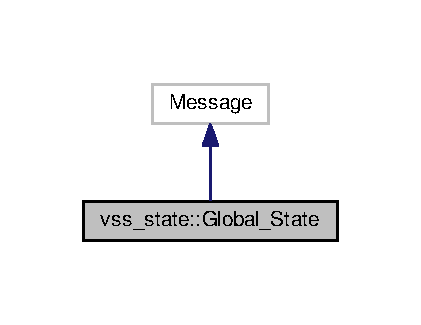
\includegraphics[width=202pt]{classvss__state_1_1Global__State__inherit__graph}
\end{center}
\end{figure}


Diagrama de colaboração para vss\+\_\+state\+:\+:Global\+\_\+\+State\+:\nopagebreak
\begin{figure}[H]
\begin{center}
\leavevmode
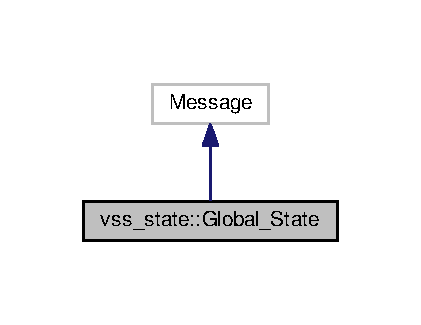
\includegraphics[width=202pt]{classvss__state_1_1Global__State__coll__graph}
\end{center}
\end{figure}
\subsection*{Métodos Públicos}
\begin{DoxyCompactItemize}
\item 
{\bfseries Global\+\_\+\+State} (const \hyperlink{classvss__state_1_1Global__State}{Global\+\_\+\+State} \&from)\hypertarget{classvss__state_1_1Global__State_a3a0a70c553656e9c3049308a9513e60c}{}\label{classvss__state_1_1Global__State_a3a0a70c553656e9c3049308a9513e60c}

\item 
\hyperlink{classvss__state_1_1Global__State}{Global\+\_\+\+State} \& {\bfseries operator=} (const \hyperlink{classvss__state_1_1Global__State}{Global\+\_\+\+State} \&from)\hypertarget{classvss__state_1_1Global__State_a01f51f37ae680992a1fd7b0aa3170af9}{}\label{classvss__state_1_1Global__State_a01f51f37ae680992a1fd7b0aa3170af9}

\item 
const \+::google\+::protobuf\+::\+Unknown\+Field\+Set \& {\bfseries unknown\+\_\+fields} () const \hypertarget{classvss__state_1_1Global__State_ad315f5c8ac8db0801d1f554b0f5220e9}{}\label{classvss__state_1_1Global__State_ad315f5c8ac8db0801d1f554b0f5220e9}

\item 
inline\+::google\+::protobuf\+::\+Unknown\+Field\+Set $\ast$ {\bfseries mutable\+\_\+unknown\+\_\+fields} ()\hypertarget{classvss__state_1_1Global__State_a4dbf780222435e650455d532b81dca44}{}\label{classvss__state_1_1Global__State_a4dbf780222435e650455d532b81dca44}

\item 
void {\bfseries Swap} (\hyperlink{classvss__state_1_1Global__State}{Global\+\_\+\+State} $\ast$other)\hypertarget{classvss__state_1_1Global__State_a2b83b57b8673e15692526e3c4ccccc94}{}\label{classvss__state_1_1Global__State_a2b83b57b8673e15692526e3c4ccccc94}

\item 
\hyperlink{classvss__state_1_1Global__State}{Global\+\_\+\+State} $\ast$ {\bfseries New} () const \hypertarget{classvss__state_1_1Global__State_a2e84bb1599128b996a43de926501d5bc}{}\label{classvss__state_1_1Global__State_a2e84bb1599128b996a43de926501d5bc}

\item 
\hyperlink{classvss__state_1_1Global__State}{Global\+\_\+\+State} $\ast$ {\bfseries New} (\+::google\+::protobuf\+::\+Arena $\ast$arena) const \hypertarget{classvss__state_1_1Global__State_a9d41a76067944912f31e2c4952fa17dd}{}\label{classvss__state_1_1Global__State_a9d41a76067944912f31e2c4952fa17dd}

\item 
void {\bfseries Copy\+From} (const \+::google\+::protobuf\+::\+Message \&from)\hypertarget{classvss__state_1_1Global__State_a5a57651faea985db08eafee9429407d0}{}\label{classvss__state_1_1Global__State_a5a57651faea985db08eafee9429407d0}

\item 
void {\bfseries Merge\+From} (const \+::google\+::protobuf\+::\+Message \&from)\hypertarget{classvss__state_1_1Global__State_ad2905d67a08d3e766963be4d20438dee}{}\label{classvss__state_1_1Global__State_ad2905d67a08d3e766963be4d20438dee}

\item 
void {\bfseries Copy\+From} (const \hyperlink{classvss__state_1_1Global__State}{Global\+\_\+\+State} \&from)\hypertarget{classvss__state_1_1Global__State_aba34386a742582208d2ead2116512710}{}\label{classvss__state_1_1Global__State_aba34386a742582208d2ead2116512710}

\item 
void {\bfseries Merge\+From} (const \hyperlink{classvss__state_1_1Global__State}{Global\+\_\+\+State} \&from)\hypertarget{classvss__state_1_1Global__State_a429e2ccd5b142708a51a3bd069455f52}{}\label{classvss__state_1_1Global__State_a429e2ccd5b142708a51a3bd069455f52}

\item 
void {\bfseries Clear} ()\hypertarget{classvss__state_1_1Global__State_a9c2d7a9cf4dd3c01b53a749e25b0d0fb}{}\label{classvss__state_1_1Global__State_a9c2d7a9cf4dd3c01b53a749e25b0d0fb}

\item 
bool {\bfseries Is\+Initialized} () const \hypertarget{classvss__state_1_1Global__State_ab2c7e2d4af0cd33383e9a4bd1a83113f}{}\label{classvss__state_1_1Global__State_ab2c7e2d4af0cd33383e9a4bd1a83113f}

\item 
int {\bfseries Byte\+Size} () const \hypertarget{classvss__state_1_1Global__State_a10790a0ee8bcc6cff1f704ad0dce113c}{}\label{classvss__state_1_1Global__State_a10790a0ee8bcc6cff1f704ad0dce113c}

\item 
bool {\bfseries Merge\+Partial\+From\+Coded\+Stream} (\+::google\+::protobuf\+::io\+::\+Coded\+Input\+Stream $\ast$input)\hypertarget{classvss__state_1_1Global__State_a6441ee848d925dd1cd3bca5e30c28c7f}{}\label{classvss__state_1_1Global__State_a6441ee848d925dd1cd3bca5e30c28c7f}

\item 
void {\bfseries Serialize\+With\+Cached\+Sizes} (\+::google\+::protobuf\+::io\+::\+Coded\+Output\+Stream $\ast$output) const \hypertarget{classvss__state_1_1Global__State_a01a832c00539c849c8171ff3a228f0df}{}\label{classvss__state_1_1Global__State_a01a832c00539c849c8171ff3a228f0df}

\item 
\+::google\+::protobuf\+::uint8 $\ast$ {\bfseries Internal\+Serialize\+With\+Cached\+Sizes\+To\+Array} (bool deterministic,\+::google\+::protobuf\+::uint8 $\ast$output) const \hypertarget{classvss__state_1_1Global__State_a8f00725e70bfba6a8ede5ed325a23a28}{}\label{classvss__state_1_1Global__State_a8f00725e70bfba6a8ede5ed325a23a28}

\item 
\+::google\+::protobuf\+::uint8 $\ast$ {\bfseries Serialize\+With\+Cached\+Sizes\+To\+Array} (\+::google\+::protobuf\+::uint8 $\ast$output) const \hypertarget{classvss__state_1_1Global__State_a4c06db3a1b1b366f5f1baa3008ff5bdb}{}\label{classvss__state_1_1Global__State_a4c06db3a1b1b366f5f1baa3008ff5bdb}

\item 
int {\bfseries Get\+Cached\+Size} () const \hypertarget{classvss__state_1_1Global__State_aa94066556db76353540b8b54d77eed2e}{}\label{classvss__state_1_1Global__State_aa94066556db76353540b8b54d77eed2e}

\item 
\+::google\+::protobuf\+::\+Metadata {\bfseries Get\+Metadata} () const \hypertarget{classvss__state_1_1Global__State_a3b2d5b30093df0eb8b20f991dc2d8d9e}{}\label{classvss__state_1_1Global__State_a3b2d5b30093df0eb8b20f991dc2d8d9e}

\item 
bool {\bfseries has\+\_\+id} () const \hypertarget{classvss__state_1_1Global__State_a7d7595f10e8923fada79b67c77ba7cd3}{}\label{classvss__state_1_1Global__State_a7d7595f10e8923fada79b67c77ba7cd3}

\item 
void {\bfseries clear\+\_\+id} ()\hypertarget{classvss__state_1_1Global__State_a0b001773d7aafdb5acef5b36c35f7075}{}\label{classvss__state_1_1Global__State_a0b001773d7aafdb5acef5b36c35f7075}

\item 
\+::google\+::protobuf\+::uint32 {\bfseries id} () const \hypertarget{classvss__state_1_1Global__State_ab0ff3c2867cdfda57429a649c9abde17}{}\label{classvss__state_1_1Global__State_ab0ff3c2867cdfda57429a649c9abde17}

\item 
void {\bfseries set\+\_\+id} (\+::google\+::protobuf\+::uint32 value)\hypertarget{classvss__state_1_1Global__State_a183935ca3daee149b526d4a50cce450e}{}\label{classvss__state_1_1Global__State_a183935ca3daee149b526d4a50cce450e}

\item 
bool {\bfseries has\+\_\+origin} () const \hypertarget{classvss__state_1_1Global__State_ab80313b62ce603f182c3e2e1fbea8da5}{}\label{classvss__state_1_1Global__State_ab80313b62ce603f182c3e2e1fbea8da5}

\item 
void {\bfseries clear\+\_\+origin} ()\hypertarget{classvss__state_1_1Global__State_a60aa49b36faa6533ed70bc9e01208282}{}\label{classvss__state_1_1Global__State_a60aa49b36faa6533ed70bc9e01208282}

\item 
bool {\bfseries origin} () const \hypertarget{classvss__state_1_1Global__State_a5b09a31922fe8f976a7e21f2279a1364}{}\label{classvss__state_1_1Global__State_a5b09a31922fe8f976a7e21f2279a1364}

\item 
void {\bfseries set\+\_\+origin} (bool value)\hypertarget{classvss__state_1_1Global__State_ac88223b795690cc57a71f24b315352fc}{}\label{classvss__state_1_1Global__State_ac88223b795690cc57a71f24b315352fc}

\item 
int {\bfseries balls\+\_\+size} () const \hypertarget{classvss__state_1_1Global__State_a5010e0f86563f07ce75ed2138de96ae5}{}\label{classvss__state_1_1Global__State_a5010e0f86563f07ce75ed2138de96ae5}

\item 
void {\bfseries clear\+\_\+balls} ()\hypertarget{classvss__state_1_1Global__State_a738a0947e2c3a450614579e1b7c008e4}{}\label{classvss__state_1_1Global__State_a738a0947e2c3a450614579e1b7c008e4}

\item 
const \+::\hyperlink{classvss__state_1_1Ball__State}{vss\+\_\+state\+::\+Ball\+\_\+\+State} \& {\bfseries balls} (int index) const \hypertarget{classvss__state_1_1Global__State_a6177a6bdab45c96d10c9f64371cd12af}{}\label{classvss__state_1_1Global__State_a6177a6bdab45c96d10c9f64371cd12af}

\item 
\+::\hyperlink{classvss__state_1_1Ball__State}{vss\+\_\+state\+::\+Ball\+\_\+\+State} $\ast$ {\bfseries mutable\+\_\+balls} (int index)\hypertarget{classvss__state_1_1Global__State_a88e1c23a1561e6edeaa2c835ad5eb358}{}\label{classvss__state_1_1Global__State_a88e1c23a1561e6edeaa2c835ad5eb358}

\item 
\+::\hyperlink{classvss__state_1_1Ball__State}{vss\+\_\+state\+::\+Ball\+\_\+\+State} $\ast$ {\bfseries add\+\_\+balls} ()\hypertarget{classvss__state_1_1Global__State_aa02eca734a92c0f8352fc57dbda91e4e}{}\label{classvss__state_1_1Global__State_aa02eca734a92c0f8352fc57dbda91e4e}

\item 
\+::google\+::protobuf\+::\+Repeated\+Ptr\+Field$<$ \+::\hyperlink{classvss__state_1_1Ball__State}{vss\+\_\+state\+::\+Ball\+\_\+\+State} $>$ $\ast$ {\bfseries mutable\+\_\+balls} ()\hypertarget{classvss__state_1_1Global__State_a47fa3f079e92555b8d86ef916def763e}{}\label{classvss__state_1_1Global__State_a47fa3f079e92555b8d86ef916def763e}

\item 
const \+::google\+::protobuf\+::\+Repeated\+Ptr\+Field$<$ \+::\hyperlink{classvss__state_1_1Ball__State}{vss\+\_\+state\+::\+Ball\+\_\+\+State} $>$ \& {\bfseries balls} () const \hypertarget{classvss__state_1_1Global__State_a792da3990e724f225e585f3e099eab3c}{}\label{classvss__state_1_1Global__State_a792da3990e724f225e585f3e099eab3c}

\item 
int {\bfseries robots\+\_\+yellow\+\_\+size} () const \hypertarget{classvss__state_1_1Global__State_ad9605aa1df1cc1a30adc6a88bd85f34f}{}\label{classvss__state_1_1Global__State_ad9605aa1df1cc1a30adc6a88bd85f34f}

\item 
void {\bfseries clear\+\_\+robots\+\_\+yellow} ()\hypertarget{classvss__state_1_1Global__State_a5519565ece84f3f429aa692217fff1f6}{}\label{classvss__state_1_1Global__State_a5519565ece84f3f429aa692217fff1f6}

\item 
const \+::\hyperlink{classvss__state_1_1Robot__State}{vss\+\_\+state\+::\+Robot\+\_\+\+State} \& {\bfseries robots\+\_\+yellow} (int index) const \hypertarget{classvss__state_1_1Global__State_a311a39a8f7be0721ebb684b9bc286ce2}{}\label{classvss__state_1_1Global__State_a311a39a8f7be0721ebb684b9bc286ce2}

\item 
\+::\hyperlink{classvss__state_1_1Robot__State}{vss\+\_\+state\+::\+Robot\+\_\+\+State} $\ast$ {\bfseries mutable\+\_\+robots\+\_\+yellow} (int index)\hypertarget{classvss__state_1_1Global__State_a040f90d8bad2e783b1e91077a7c79234}{}\label{classvss__state_1_1Global__State_a040f90d8bad2e783b1e91077a7c79234}

\item 
\+::\hyperlink{classvss__state_1_1Robot__State}{vss\+\_\+state\+::\+Robot\+\_\+\+State} $\ast$ {\bfseries add\+\_\+robots\+\_\+yellow} ()\hypertarget{classvss__state_1_1Global__State_aecf340a8be8a26db65bd29ebafcbf1d6}{}\label{classvss__state_1_1Global__State_aecf340a8be8a26db65bd29ebafcbf1d6}

\item 
\+::google\+::protobuf\+::\+Repeated\+Ptr\+Field$<$ \+::\hyperlink{classvss__state_1_1Robot__State}{vss\+\_\+state\+::\+Robot\+\_\+\+State} $>$ $\ast$ {\bfseries mutable\+\_\+robots\+\_\+yellow} ()\hypertarget{classvss__state_1_1Global__State_a533514002331b04a673326f334a3e5ce}{}\label{classvss__state_1_1Global__State_a533514002331b04a673326f334a3e5ce}

\item 
const \+::google\+::protobuf\+::\+Repeated\+Ptr\+Field$<$ \+::\hyperlink{classvss__state_1_1Robot__State}{vss\+\_\+state\+::\+Robot\+\_\+\+State} $>$ \& {\bfseries robots\+\_\+yellow} () const \hypertarget{classvss__state_1_1Global__State_ad18fe89214728e2c808c8911575ab90b}{}\label{classvss__state_1_1Global__State_ad18fe89214728e2c808c8911575ab90b}

\item 
int {\bfseries robots\+\_\+blue\+\_\+size} () const \hypertarget{classvss__state_1_1Global__State_ab19e999740e3aa72946a92322bc7f163}{}\label{classvss__state_1_1Global__State_ab19e999740e3aa72946a92322bc7f163}

\item 
void {\bfseries clear\+\_\+robots\+\_\+blue} ()\hypertarget{classvss__state_1_1Global__State_ae88bcfb62ea5ea68673a48aaec873723}{}\label{classvss__state_1_1Global__State_ae88bcfb62ea5ea68673a48aaec873723}

\item 
const \+::\hyperlink{classvss__state_1_1Robot__State}{vss\+\_\+state\+::\+Robot\+\_\+\+State} \& {\bfseries robots\+\_\+blue} (int index) const \hypertarget{classvss__state_1_1Global__State_a92551a5a96b8585f89cc37c55b0c4e46}{}\label{classvss__state_1_1Global__State_a92551a5a96b8585f89cc37c55b0c4e46}

\item 
\+::\hyperlink{classvss__state_1_1Robot__State}{vss\+\_\+state\+::\+Robot\+\_\+\+State} $\ast$ {\bfseries mutable\+\_\+robots\+\_\+blue} (int index)\hypertarget{classvss__state_1_1Global__State_a1caf337906ddf4fa47b606dc76cd8a3b}{}\label{classvss__state_1_1Global__State_a1caf337906ddf4fa47b606dc76cd8a3b}

\item 
\+::\hyperlink{classvss__state_1_1Robot__State}{vss\+\_\+state\+::\+Robot\+\_\+\+State} $\ast$ {\bfseries add\+\_\+robots\+\_\+blue} ()\hypertarget{classvss__state_1_1Global__State_a3150ca6510afc0a88b10491642dff24a}{}\label{classvss__state_1_1Global__State_a3150ca6510afc0a88b10491642dff24a}

\item 
\+::google\+::protobuf\+::\+Repeated\+Ptr\+Field$<$ \+::\hyperlink{classvss__state_1_1Robot__State}{vss\+\_\+state\+::\+Robot\+\_\+\+State} $>$ $\ast$ {\bfseries mutable\+\_\+robots\+\_\+blue} ()\hypertarget{classvss__state_1_1Global__State_a73be200ff11edfc042221b579672d3b4}{}\label{classvss__state_1_1Global__State_a73be200ff11edfc042221b579672d3b4}

\item 
const \+::google\+::protobuf\+::\+Repeated\+Ptr\+Field$<$ \+::\hyperlink{classvss__state_1_1Robot__State}{vss\+\_\+state\+::\+Robot\+\_\+\+State} $>$ \& {\bfseries robots\+\_\+blue} () const \hypertarget{classvss__state_1_1Global__State_ad659e30adf37a0e412765337eb28f233}{}\label{classvss__state_1_1Global__State_ad659e30adf37a0e412765337eb28f233}

\item 
bool {\bfseries has\+\_\+situation} () const \hypertarget{classvss__state_1_1Global__State_a261f48529a5cb4bc9d4cc9ba645e530b}{}\label{classvss__state_1_1Global__State_a261f48529a5cb4bc9d4cc9ba645e530b}

\item 
void {\bfseries clear\+\_\+situation} ()\hypertarget{classvss__state_1_1Global__State_a1b8e5668d373349fa5a7d8bfeb299057}{}\label{classvss__state_1_1Global__State_a1b8e5668d373349fa5a7d8bfeb299057}

\item 
\+::google\+::protobuf\+::uint32 {\bfseries situation} () const \hypertarget{classvss__state_1_1Global__State_a02c6e5b10b81236b46bfce5b2d245d40}{}\label{classvss__state_1_1Global__State_a02c6e5b10b81236b46bfce5b2d245d40}

\item 
void {\bfseries set\+\_\+situation} (\+::google\+::protobuf\+::uint32 value)\hypertarget{classvss__state_1_1Global__State_a111561db5dbd32a5daa13893ddaa297c}{}\label{classvss__state_1_1Global__State_a111561db5dbd32a5daa13893ddaa297c}

\end{DoxyCompactItemize}
\subsection*{Métodos Públicos Estáticos}
\begin{DoxyCompactItemize}
\item 
static const \+::google\+::protobuf\+::\+Descriptor $\ast$ {\bfseries descriptor} ()\hypertarget{classvss__state_1_1Global__State_af5963eb38d472f2508e180fdf42c4a22}{}\label{classvss__state_1_1Global__State_af5963eb38d472f2508e180fdf42c4a22}

\item 
static const \hyperlink{classvss__state_1_1Global__State}{Global\+\_\+\+State} \& {\bfseries default\+\_\+instance} ()\hypertarget{classvss__state_1_1Global__State_a1bf08b600180f360bcd37c58f3e50b16}{}\label{classvss__state_1_1Global__State_a1bf08b600180f360bcd37c58f3e50b16}

\end{DoxyCompactItemize}
\subsection*{Atributos Estáticos Públicos}
\begin{DoxyCompactItemize}
\item 
static const int {\bfseries k\+Id\+Field\+Number} = 1\hypertarget{classvss__state_1_1Global__State_adc3acf2d9111dd7e0e442b1c8f8743ab}{}\label{classvss__state_1_1Global__State_adc3acf2d9111dd7e0e442b1c8f8743ab}

\item 
static const int {\bfseries k\+Origin\+Field\+Number} = 2\hypertarget{classvss__state_1_1Global__State_a124e80222f404a8607d383c6b626b98a}{}\label{classvss__state_1_1Global__State_a124e80222f404a8607d383c6b626b98a}

\item 
static const int {\bfseries k\+Balls\+Field\+Number} = 3\hypertarget{classvss__state_1_1Global__State_a7ccc5ad24ae6460151ee94fd5f3800f5}{}\label{classvss__state_1_1Global__State_a7ccc5ad24ae6460151ee94fd5f3800f5}

\item 
static const int {\bfseries k\+Robots\+Yellow\+Field\+Number} = 4\hypertarget{classvss__state_1_1Global__State_a3dbd17117a81ad417c69ca945668edaa}{}\label{classvss__state_1_1Global__State_a3dbd17117a81ad417c69ca945668edaa}

\item 
static const int {\bfseries k\+Robots\+Blue\+Field\+Number} = 5\hypertarget{classvss__state_1_1Global__State_a69fd6df3aa2671364cb92838e3824e81}{}\label{classvss__state_1_1Global__State_a69fd6df3aa2671364cb92838e3824e81}

\item 
static const int {\bfseries k\+Situation\+Field\+Number} = 6\hypertarget{classvss__state_1_1Global__State_a2d5cf9ac7fcb6fd41d98c14ce50ff2ac}{}\label{classvss__state_1_1Global__State_a2d5cf9ac7fcb6fd41d98c14ce50ff2ac}

\end{DoxyCompactItemize}
\subsection*{Amigas}
\begin{DoxyCompactItemize}
\item 
void {\bfseries protobuf\+\_\+\+Add\+Desc\+\_\+state\+\_\+2eproto} ()\hypertarget{classvss__state_1_1Global__State_aab1a2c258f8122a403a979ff57e2a706}{}\label{classvss__state_1_1Global__State_aab1a2c258f8122a403a979ff57e2a706}

\item 
void {\bfseries protobuf\+\_\+\+Assign\+Desc\+\_\+state\+\_\+2eproto} ()\hypertarget{classvss__state_1_1Global__State_a57d9367bc8a7a94ead11d11194cca1b6}{}\label{classvss__state_1_1Global__State_a57d9367bc8a7a94ead11d11194cca1b6}

\item 
void {\bfseries protobuf\+\_\+\+Shutdown\+File\+\_\+state\+\_\+2eproto} ()\hypertarget{classvss__state_1_1Global__State_a4e6dc5e8e72799859c4e9556d090e57d}{}\label{classvss__state_1_1Global__State_a4e6dc5e8e72799859c4e9556d090e57d}

\end{DoxyCompactItemize}


A documentação para esta classe foi gerada a partir dos seguintes arquivos\+:\begin{DoxyCompactItemize}
\item 
/home/johnathan/\+Repositories/\+S\+I\+R\+Lab/\+Public/\+V\+S\+S-\/\+Viewer/src/\+V\+S\+S-\/\+Interface/protos/state.\+pb.\+h\item 
/home/johnathan/\+Repositories/\+S\+I\+R\+Lab/\+Public/\+V\+S\+S-\/\+Viewer/src/\+V\+S\+S-\/\+Interface/protos/state.\+pb.\+cc\end{DoxyCompactItemize}

\hypertarget{classGraphics}{}\section{Referência da Classe Graphics}
\label{classGraphics}\index{Graphics@{Graphics}}


Essa classe é responsável por desenhar o mundo 3D e receber os estados do V\+S\+S-\/\+Simulator e V\+S\+S-\/\+Vision.  




{\ttfamily \#include $<$graphics.\+h$>$}



Diagrama de colaboração para Graphics\+:\nopagebreak
\begin{figure}[H]
\begin{center}
\leavevmode
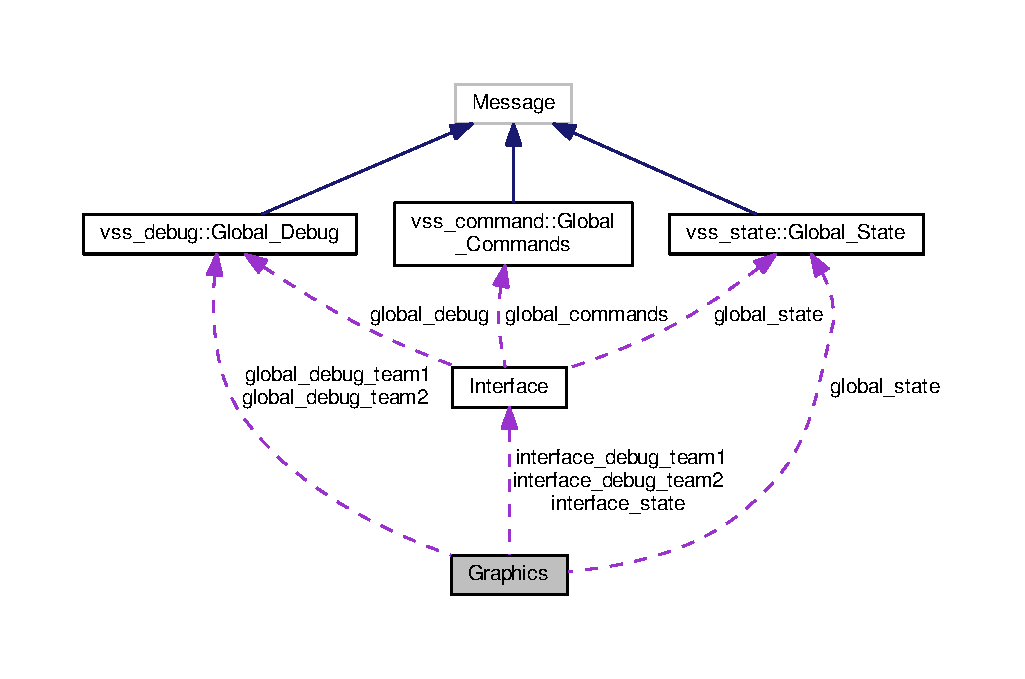
\includegraphics[width=350pt]{classGraphics__coll__graph}
\end{center}
\end{figure}
\subsection*{Métodos Públicos}
\begin{DoxyCompactItemize}
\item 
\hyperlink{classGraphics_af2e8fe67fd31ec263c843a6e28b29d3c}{Graphics} ()
\begin{DoxyCompactList}\small\item\em Construtor D\+E\+F\+A\+U\+LT. \end{DoxyCompactList}\item 
void \hyperlink{classGraphics_aa1cd9918be0133bb6cf59de07ee211f8}{init} (int \hyperlink{classGraphics_a1b1e8eba7ed4e60d78d785e70765fef6}{argc}, char $\ast$$\ast$\hyperlink{classGraphics_aca7bf0128e62af000265c0e66ed5e7e1}{argv}, bool \hyperlink{classGraphics_a16b588a2b580e104d18c347f8318e3bd}{debug}, string \hyperlink{classGraphics_acb397e43edd9c7d6de193bbb9ff55b94}{camera}, string \hyperlink{classGraphics_ad5daf3bff501ac78b1507a8df1534423}{ip})
\begin{DoxyCompactList}\small\item\em Método responsável por inicializar o software. \end{DoxyCompactList}\item 
void \hyperlink{classGraphics_a5c2dc0d8c33e87def636d4edce50f4a5}{draw\+\_\+thread} ()
\begin{DoxyCompactList}\small\item\em Método responsável por carregar a thread de desenho. \end{DoxyCompactList}\item 
void \hyperlink{classGraphics_a6429fd2fc5fa7a3c5a56b9987e13afdb}{state\+\_\+thread} ()
\begin{DoxyCompactList}\small\item\em Metodo responsável por carregar a thread de recebimento de estados do V\+S\+S-\/\+Vision e V\+S\+S-\/\+Simulator. \end{DoxyCompactList}\item 
void \hyperlink{classGraphics_af5bddf0e5aecdf97e779efa677b2179b}{debug\+\_\+thread\+\_\+team1} ()
\begin{DoxyCompactList}\small\item\em Método responsável por carregar a thread de recebimento de informações de debug do time1. \end{DoxyCompactList}\item 
void \hyperlink{classGraphics_aee35712f5483009df689c313df804f52}{debug\+\_\+thread\+\_\+team2} ()
\begin{DoxyCompactList}\small\item\em Método responsável por carregar a thread de recebimento de informações de debug do time2. \end{DoxyCompactList}\end{DoxyCompactItemize}
\subsection*{Métodos Públicos Estáticos}
\begin{DoxyCompactItemize}
\item 
static void \hyperlink{classGraphics_ab65394158d2a2fa6a613fcb074ac808e}{draw\+World} ()
\begin{DoxyCompactList}\small\item\em Método responsável por desenhar o ambiente 3D. \end{DoxyCompactList}\item 
static void \hyperlink{classGraphics_a3549ba0484b18d43c6602fb0b57a29a6}{init\+Light} ()\hypertarget{classGraphics_a3549ba0484b18d43c6602fb0b57a29a6}{}\label{classGraphics_a3549ba0484b18d43c6602fb0b57a29a6}

\begin{DoxyCompactList}\small\item\em Método responsável por definir a luz ambiente, difusa, especular e a posição. \end{DoxyCompactList}\item 
static void \hyperlink{classGraphics_aa2795786eef8c99a7232a195992a9c82}{timer\+Handler} (int v)
\begin{DoxyCompactList}\small\item\em Método (Callback) responsável por redesenhar o mundo 3D mantendo ao menos 30 Fps. \end{DoxyCompactList}\item 
static void \hyperlink{classGraphics_a78ef6a0b1f6c142c9d650ffddfbaa2ed}{change\+Window\+Size} (G\+Lsizei w, G\+Lsizei h)\hypertarget{classGraphics_a78ef6a0b1f6c142c9d650ffddfbaa2ed}{}\label{classGraphics_a78ef6a0b1f6c142c9d650ffddfbaa2ed}

\begin{DoxyCompactList}\small\item\em Método (Callback) responsável por atualizar as váriaveis de controle se o usuário mudar o tamanho da janela. \end{DoxyCompactList}\item 
static void \hyperlink{classGraphics_ab3134b5ca29b658f4ac5cc12fa4b4705}{material} (int color=B\+L\+A\+CK)\hypertarget{classGraphics_ab3134b5ca29b658f4ac5cc12fa4b4705}{}\label{classGraphics_ab3134b5ca29b658f4ac5cc12fa4b4705}

\begin{DoxyCompactList}\small\item\em Método responsável for definir a cor 3D do material\+: O\+R\+A\+N\+GE, B\+L\+UE, Y\+E\+L\+L\+OW, R\+ED, G\+R\+E\+EN, P\+U\+R\+P\+LE, P\+I\+NK, B\+R\+O\+WN, W\+H\+I\+TE, G\+R\+AY, B\+L\+A\+CK, B\+L\+A\+C\+K2, B\+L\+A\+C\+K3. \end{DoxyCompactList}\item 
static void \hyperlink{classGraphics_a7fccb7730e87ee29133bc0fa6171059e}{material} (\hyperlink{structcommon_1_1Pixel}{Pixel})
\begin{DoxyCompactList}\small\item\em Método responsável por definir a cor 3D do material, recebendo um valor R\+GB. \end{DoxyCompactList}\item 
static void \hyperlink{classGraphics_ab5d975a404218d57cd494b8897d7b046}{material3f} (int color=B\+L\+A\+CK)
\begin{DoxyCompactList}\small\item\em Método responsável por definir a cor 2D do material\+: O\+R\+A\+N\+GE, B\+L\+UE, Y\+E\+L\+L\+OW, R\+ED, G\+R\+E\+EN, P\+U\+R\+P\+LE, P\+I\+NK, B\+R\+O\+WN, W\+H\+I\+TE, G\+R\+AY, B\+L\+A\+CK, B\+L\+A\+C\+K2, B\+L\+A\+C\+K3. \end{DoxyCompactList}\item 
static void \hyperlink{classGraphics_a23d042e2b5a049bb2369d9a1f6794e2d}{material3f} (\hyperlink{structcommon_1_1Pixel}{Pixel})\hypertarget{classGraphics_a23d042e2b5a049bb2369d9a1f6794e2d}{}\label{classGraphics_a23d042e2b5a049bb2369d9a1f6794e2d}

\begin{DoxyCompactList}\small\item\em Método responsável por definir a cor 2D do material, recebendo um valor R\+GB. \end{DoxyCompactList}\item 
static void \hyperlink{classGraphics_adc5dbcd8d8d999d48dbdf241fde77603}{draw\+Field} ()\hypertarget{classGraphics_adc5dbcd8d8d999d48dbdf241fde77603}{}\label{classGraphics_adc5dbcd8d8d999d48dbdf241fde77603}

\begin{DoxyCompactList}\small\item\em Método responsável por desenhar o campo\+: chão e paredes. \end{DoxyCompactList}\item 
static void \hyperlink{classGraphics_aea303675636309a511de1b2158cb1105}{draw\+Robot} (int)
\begin{DoxyCompactList}\small\item\em Método responsável desenhar um robô\+: corpo e rodas. \end{DoxyCompactList}\item 
static void \hyperlink{classGraphics_a9cb884049d4318fd4f0ee57f293d5281}{draw\+Debug\+Final\+Robot} (int)
\begin{DoxyCompactList}\small\item\em Método responsável por desenhar a pose final de um robô \end{DoxyCompactList}\item 
static void \hyperlink{classGraphics_a9109b4c601fa113e416842d1fb98cc33}{draw\+Debug\+Step\+Robot} (int)
\begin{DoxyCompactList}\small\item\em Método responsável por desenhar o vetor de movimento de um robô \end{DoxyCompactList}\item 
static void \hyperlink{classGraphics_a19c836249f27f13ae686f33819699047}{draw\+Debug\+Path} (int)
\begin{DoxyCompactList}\small\item\em Método responsável por desennhar um caminho de um robô \end{DoxyCompactList}\item 
static void \hyperlink{classGraphics_a8e0114e205ef00c6284ed40f14cea84a}{draw\+Ball} ()\hypertarget{classGraphics_a8e0114e205ef00c6284ed40f14cea84a}{}\label{classGraphics_a8e0114e205ef00c6284ed40f14cea84a}

\begin{DoxyCompactList}\small\item\em Método responsável por desenhar a bola. \end{DoxyCompactList}\item 
static void \hyperlink{classGraphics_a099efcc1425c088c977a405c5065fcd3}{draw\+Debug\+Future\+Ball} ()
\begin{DoxyCompactList}\small\item\em Método responsável por desenhar a bola no futuro. \end{DoxyCompactList}\end{DoxyCompactItemize}
\subsection*{Atributos Protegidos}
\begin{DoxyCompactItemize}
\item 
int \hyperlink{classGraphics_a1b1e8eba7ed4e60d78d785e70765fef6}{argc}\hypertarget{classGraphics_a1b1e8eba7ed4e60d78d785e70765fef6}{}\label{classGraphics_a1b1e8eba7ed4e60d78d785e70765fef6}

\begin{DoxyCompactList}\small\item\em Parâmetro utilizado pela Glut. \end{DoxyCompactList}\item 
char $\ast$$\ast$ \hyperlink{classGraphics_aca7bf0128e62af000265c0e66ed5e7e1}{argv}\hypertarget{classGraphics_aca7bf0128e62af000265c0e66ed5e7e1}{}\label{classGraphics_aca7bf0128e62af000265c0e66ed5e7e1}

\begin{DoxyCompactList}\small\item\em Parâmetro utilizado pela Glut. \end{DoxyCompactList}\item 
bool \hyperlink{classGraphics_a16b588a2b580e104d18c347f8318e3bd}{debug}\hypertarget{classGraphics_a16b588a2b580e104d18c347f8318e3bd}{}\label{classGraphics_a16b588a2b580e104d18c347f8318e3bd}

\begin{DoxyCompactList}\small\item\em Define se debug está ligado ou não. \end{DoxyCompactList}\item 
string \hyperlink{classGraphics_acb397e43edd9c7d6de193bbb9ff55b94}{camera}\hypertarget{classGraphics_acb397e43edd9c7d6de193bbb9ff55b94}{}\label{classGraphics_acb397e43edd9c7d6de193bbb9ff55b94}

\begin{DoxyCompactList}\small\item\em Câmera utilizada\+: TV ou T\+O\+PO. \end{DoxyCompactList}\item 
string \hyperlink{classGraphics_ad5daf3bff501ac78b1507a8df1534423}{ip}\hypertarget{classGraphics_ad5daf3bff501ac78b1507a8df1534423}{}\label{classGraphics_ad5daf3bff501ac78b1507a8df1534423}

\begin{DoxyCompactList}\small\item\em Ip do PC que esteja rodando o V\+S\+S-\/\+Vision ou V\+S\+S-\/\+Simulator. Por D\+E\+F\+A\+U\+LT é localhost ou 127.\+0.\+0.\+1. \end{DoxyCompactList}\item 
float \hyperlink{classGraphics_a5b0018455ff1e2ab3d43d1446cfdfe4d}{width}\hypertarget{classGraphics_a5b0018455ff1e2ab3d43d1446cfdfe4d}{}\label{classGraphics_a5b0018455ff1e2ab3d43d1446cfdfe4d}

\begin{DoxyCompactList}\small\item\em Largura da janela de desenho. \end{DoxyCompactList}\item 
float \hyperlink{classGraphics_a47cbc0011a0a10476fec75d62d7e0fcf}{height}\hypertarget{classGraphics_a47cbc0011a0a10476fec75d62d7e0fcf}{}\label{classGraphics_a47cbc0011a0a10476fec75d62d7e0fcf}

\begin{DoxyCompactList}\small\item\em Altura da janela de desenho. \end{DoxyCompactList}\item 
thread $\ast$ \hyperlink{classGraphics_ac8094b0bd8b0962735f5fdebb7b70f53}{thread\+\_\+draw}\hypertarget{classGraphics_ac8094b0bd8b0962735f5fdebb7b70f53}{}\label{classGraphics_ac8094b0bd8b0962735f5fdebb7b70f53}

\begin{DoxyCompactList}\small\item\em Thread responsável para desenhar o ambiente. \end{DoxyCompactList}\item 
thread $\ast$ \hyperlink{classGraphics_a202be3ede52a05610cdd075e018e69ae}{thread\+\_\+state}\hypertarget{classGraphics_a202be3ede52a05610cdd075e018e69ae}{}\label{classGraphics_a202be3ede52a05610cdd075e018e69ae}

\begin{DoxyCompactList}\small\item\em Thread responsável por receber os estados do V\+S\+S-\/\+Vision e V\+S\+S-\/\+Simulator. \end{DoxyCompactList}\item 
thread $\ast$ \hyperlink{classGraphics_a291d3fb993aaf96ffe574ce850ef147f}{thread\+\_\+debug\+\_\+team1}\hypertarget{classGraphics_a291d3fb993aaf96ffe574ce850ef147f}{}\label{classGraphics_a291d3fb993aaf96ffe574ce850ef147f}

\begin{DoxyCompactList}\small\item\em Thread responsável por receber os pacotes de debug do time amarelo. \end{DoxyCompactList}\item 
thread $\ast$ \hyperlink{classGraphics_af5011e9e4e9a8eddbf1d1a75156c8f7e}{thread\+\_\+debug\+\_\+team2}\hypertarget{classGraphics_af5011e9e4e9a8eddbf1d1a75156c8f7e}{}\label{classGraphics_af5011e9e4e9a8eddbf1d1a75156c8f7e}

\begin{DoxyCompactList}\small\item\em Thread responsável por receber os pacotes de debug do time azul. \end{DoxyCompactList}\item 
\hyperlink{classInterface}{Interface} \hyperlink{classGraphics_a3c5730bb3f5bda9d0727ab14fa3af068}{interface\+\_\+state}\hypertarget{classGraphics_a3c5730bb3f5bda9d0727ab14fa3af068}{}\label{classGraphics_a3c5730bb3f5bda9d0727ab14fa3af068}

\begin{DoxyCompactList}\small\item\em \hyperlink{classInterface}{Interface} de comunicação responsável por receber estados do V\+S\+S-\/\+Vision e V\+S\+S-\/\+Simulator. \end{DoxyCompactList}\item 
\hyperlink{classInterface}{Interface} \hyperlink{classGraphics_a6580b42a3da603d5fc8a40939d518b34}{interface\+\_\+debug\+\_\+team1}\hypertarget{classGraphics_a6580b42a3da603d5fc8a40939d518b34}{}\label{classGraphics_a6580b42a3da603d5fc8a40939d518b34}

\begin{DoxyCompactList}\small\item\em \hyperlink{classInterface}{Interface} de comunicação responsável por receber os pacotes de debug do time amarelo. \end{DoxyCompactList}\item 
\hyperlink{classInterface}{Interface} \hyperlink{classGraphics_a39fd7caa133ce1ad55c527b72812e338}{interface\+\_\+debug\+\_\+team2}\hypertarget{classGraphics_a39fd7caa133ce1ad55c527b72812e338}{}\label{classGraphics_a39fd7caa133ce1ad55c527b72812e338}

\begin{DoxyCompactList}\small\item\em \hyperlink{classInterface}{Interface} de comunicação responsável por receber os pacotes de debug do time azul. \end{DoxyCompactList}\item 
\hyperlink{classvss__state_1_1Global__State}{vss\+\_\+state\+::\+Global\+\_\+\+State} \hyperlink{classGraphics_a319be43d30ac19e414dbc1c3fdb336dc}{global\+\_\+state}\hypertarget{classGraphics_a319be43d30ac19e414dbc1c3fdb336dc}{}\label{classGraphics_a319be43d30ac19e414dbc1c3fdb336dc}

\begin{DoxyCompactList}\small\item\em Pacote que carrega os estados do V\+S\+S-\/\+Vision e V\+S\+S-\/\+Simulator. \end{DoxyCompactList}\item 
\hyperlink{classvss__debug_1_1Global__Debug}{vss\+\_\+debug\+::\+Global\+\_\+\+Debug} \hyperlink{classGraphics_adc864f47fef1f3d4af3f7ee5099d20da}{global\+\_\+debug\+\_\+team1}\hypertarget{classGraphics_adc864f47fef1f3d4af3f7ee5099d20da}{}\label{classGraphics_adc864f47fef1f3d4af3f7ee5099d20da}

\begin{DoxyCompactList}\small\item\em Pacote que carrega as informações de debug do time amarelo. \end{DoxyCompactList}\item 
\hyperlink{classvss__debug_1_1Global__Debug}{vss\+\_\+debug\+::\+Global\+\_\+\+Debug} \hyperlink{classGraphics_a8844312f48a5062d0b86d5eb16aecd6e}{global\+\_\+debug\+\_\+team2}\hypertarget{classGraphics_a8844312f48a5062d0b86d5eb16aecd6e}{}\label{classGraphics_a8844312f48a5062d0b86d5eb16aecd6e}

\begin{DoxyCompactList}\small\item\em Pacote que carrega as informações de debug do time azul. \end{DoxyCompactList}\end{DoxyCompactItemize}


\subsection{Descrição Detalhada}
Essa classe é responsável por desenhar o mundo 3D e receber os estados do V\+S\+S-\/\+Simulator e V\+S\+S-\/\+Vision. 

\subsection{Construtores \& Destrutores}
\index{Graphics@{Graphics}!Graphics@{Graphics}}
\index{Graphics@{Graphics}!Graphics@{Graphics}}
\subsubsection[{\texorpdfstring{Graphics()}{Graphics()}}]{\setlength{\rightskip}{0pt plus 5cm}Graphics\+::\+Graphics (
\begin{DoxyParamCaption}
{}
\end{DoxyParamCaption}
)}\hypertarget{classGraphics_af2e8fe67fd31ec263c843a6e28b29d3c}{}\label{classGraphics_af2e8fe67fd31ec263c843a6e28b29d3c}


Construtor D\+E\+F\+A\+U\+LT. 

Inicializa o vector de robôs com valores default. O software tem o conceito de times Inicializa o time 1

Inicializa o time 2 

\subsection{Métodos}
\index{Graphics@{Graphics}!debug\+\_\+thread\+\_\+team1@{debug\+\_\+thread\+\_\+team1}}
\index{debug\+\_\+thread\+\_\+team1@{debug\+\_\+thread\+\_\+team1}!Graphics@{Graphics}}
\subsubsection[{\texorpdfstring{debug\+\_\+thread\+\_\+team1()}{debug_thread_team1()}}]{\setlength{\rightskip}{0pt plus 5cm}void Graphics\+::debug\+\_\+thread\+\_\+team1 (
\begin{DoxyParamCaption}
{}
\end{DoxyParamCaption}
)}\hypertarget{classGraphics_af5bddf0e5aecdf97e779efa677b2179b}{}\label{classGraphics_af5bddf0e5aecdf97e779efa677b2179b}


Método responsável por carregar a thread de recebimento de informações de debug do time1. 

Inicializa o recebimento de debug do time amarelo

Recebe um pacote novo

Recebe os vetores de movimento

Recebe as poses finais

Recebe os caminhos \index{Graphics@{Graphics}!debug\+\_\+thread\+\_\+team2@{debug\+\_\+thread\+\_\+team2}}
\index{debug\+\_\+thread\+\_\+team2@{debug\+\_\+thread\+\_\+team2}!Graphics@{Graphics}}
\subsubsection[{\texorpdfstring{debug\+\_\+thread\+\_\+team2()}{debug_thread_team2()}}]{\setlength{\rightskip}{0pt plus 5cm}void Graphics\+::debug\+\_\+thread\+\_\+team2 (
\begin{DoxyParamCaption}
{}
\end{DoxyParamCaption}
)}\hypertarget{classGraphics_aee35712f5483009df689c313df804f52}{}\label{classGraphics_aee35712f5483009df689c313df804f52}


Método responsável por carregar a thread de recebimento de informações de debug do time2. 

Inicializa o recebimento de debug do time azul

Recebe um pacote novo

Recebe os vetores de movimento

Recebe as poses finais

Recebe os caminhos \index{Graphics@{Graphics}!draw\+\_\+thread@{draw\+\_\+thread}}
\index{draw\+\_\+thread@{draw\+\_\+thread}!Graphics@{Graphics}}
\subsubsection[{\texorpdfstring{draw\+\_\+thread()}{draw_thread()}}]{\setlength{\rightskip}{0pt plus 5cm}void Graphics\+::draw\+\_\+thread (
\begin{DoxyParamCaption}
{}
\end{DoxyParamCaption}
)}\hypertarget{classGraphics_a5c2dc0d8c33e87def636d4edce50f4a5}{}\label{classGraphics_a5c2dc0d8c33e87def636d4edce50f4a5}


Método responsável por carregar a thread de desenho. 

Define todas as callbacks e variáveis de controle. qobj é utilizado para desenhar as rodas \index{Graphics@{Graphics}!draw\+Debug\+Final\+Robot@{draw\+Debug\+Final\+Robot}}
\index{draw\+Debug\+Final\+Robot@{draw\+Debug\+Final\+Robot}!Graphics@{Graphics}}
\subsubsection[{\texorpdfstring{draw\+Debug\+Final\+Robot(int)}{drawDebugFinalRobot(int)}}]{\setlength{\rightskip}{0pt plus 5cm}void Graphics\+::draw\+Debug\+Final\+Robot (
\begin{DoxyParamCaption}
\item[{int}]{i}
\end{DoxyParamCaption}
)\hspace{0.3cm}{\ttfamily [static]}}\hypertarget{classGraphics_a9cb884049d4318fd4f0ee57f293d5281}{}\label{classGraphics_a9cb884049d4318fd4f0ee57f293d5281}


Método responsável por desenhar a pose final de um robô 

Desenha a pose final de um robô Desenha o corpo do robô transladado

Desenha a etiqueta do time

Desenha a etiqueta secundária do robô

Utiliza cores pré-\/definidas. Utilizado se obtém dados do V\+S\+S-\/\+Simulator

Utiliza cores R\+GB. Utilizado se obtém os dados do V\+S\+S-\/\+Vision \index{Graphics@{Graphics}!draw\+Debug\+Future\+Ball@{draw\+Debug\+Future\+Ball}}
\index{draw\+Debug\+Future\+Ball@{draw\+Debug\+Future\+Ball}!Graphics@{Graphics}}
\subsubsection[{\texorpdfstring{draw\+Debug\+Future\+Ball()}{drawDebugFutureBall()}}]{\setlength{\rightskip}{0pt plus 5cm}void Graphics\+::draw\+Debug\+Future\+Ball (
\begin{DoxyParamCaption}
{}
\end{DoxyParamCaption}
)\hspace{0.3cm}{\ttfamily [static]}}\hypertarget{classGraphics_a099efcc1425c088c977a405c5065fcd3}{}\label{classGraphics_a099efcc1425c088c977a405c5065fcd3}


Método responsável por desenhar a bola no futuro. 

Desenha a bola em uma origem \index{Graphics@{Graphics}!draw\+Debug\+Path@{draw\+Debug\+Path}}
\index{draw\+Debug\+Path@{draw\+Debug\+Path}!Graphics@{Graphics}}
\subsubsection[{\texorpdfstring{draw\+Debug\+Path(int)}{drawDebugPath(int)}}]{\setlength{\rightskip}{0pt plus 5cm}void Graphics\+::draw\+Debug\+Path (
\begin{DoxyParamCaption}
\item[{int}]{i}
\end{DoxyParamCaption}
)\hspace{0.3cm}{\ttfamily [static]}}\hypertarget{classGraphics_a19c836249f27f13ae686f33819699047}{}\label{classGraphics_a19c836249f27f13ae686f33819699047}


Método responsável por desennhar um caminho de um robô 

Desenha um caminho. \index{Graphics@{Graphics}!draw\+Debug\+Step\+Robot@{draw\+Debug\+Step\+Robot}}
\index{draw\+Debug\+Step\+Robot@{draw\+Debug\+Step\+Robot}!Graphics@{Graphics}}
\subsubsection[{\texorpdfstring{draw\+Debug\+Step\+Robot(int)}{drawDebugStepRobot(int)}}]{\setlength{\rightskip}{0pt plus 5cm}void Graphics\+::draw\+Debug\+Step\+Robot (
\begin{DoxyParamCaption}
\item[{int}]{i}
\end{DoxyParamCaption}
)\hspace{0.3cm}{\ttfamily [static]}}\hypertarget{classGraphics_a9109b4c601fa113e416842d1fb98cc33}{}\label{classGraphics_a9109b4c601fa113e416842d1fb98cc33}


Método responsável por desenhar o vetor de movimento de um robô 

Desenha um vetor de movimento. \index{Graphics@{Graphics}!draw\+Robot@{draw\+Robot}}
\index{draw\+Robot@{draw\+Robot}!Graphics@{Graphics}}
\subsubsection[{\texorpdfstring{draw\+Robot(int)}{drawRobot(int)}}]{\setlength{\rightskip}{0pt plus 5cm}void Graphics\+::draw\+Robot (
\begin{DoxyParamCaption}
\item[{int}]{i}
\end{DoxyParamCaption}
)\hspace{0.3cm}{\ttfamily [static]}}\hypertarget{classGraphics_aea303675636309a511de1b2158cb1105}{}\label{classGraphics_aea303675636309a511de1b2158cb1105}


Método responsável desenhar um robô\+: corpo e rodas. 

Desenha o robô i. Desenha o corpo do robô

Desenha a etiqueta do time. Azul ou Amarelo

Desenha a segunda etiqueta do robô

Utiliza cores pré-\/definidas. Utilizado se obtém dados do V\+S\+S-\/\+Simulator

Utiliza cores R\+GB. Utilizado se obtém os dados do V\+S\+S-\/\+Vision

Desenha as rodas de um robô \index{Graphics@{Graphics}!draw\+World@{draw\+World}}
\index{draw\+World@{draw\+World}!Graphics@{Graphics}}
\subsubsection[{\texorpdfstring{draw\+World()}{drawWorld()}}]{\setlength{\rightskip}{0pt plus 5cm}void Graphics\+::draw\+World (
\begin{DoxyParamCaption}
\item[{void}]{}
\end{DoxyParamCaption}
)\hspace{0.3cm}{\ttfamily [static]}}\hypertarget{classGraphics_ab65394158d2a2fa6a613fcb074ac808e}{}\label{classGraphics_ab65394158d2a2fa6a613fcb074ac808e}


Método responsável por desenhar o ambiente 3D. 

Define a posição da camera como TV

Define a posição da camera como T\+O\+PO

Desenha campo

Desenha a bola

Desenha as informações de debug

Desenha a posição futura da bola \index{Graphics@{Graphics}!init@{init}}
\index{init@{init}!Graphics@{Graphics}}
\subsubsection[{\texorpdfstring{init(int argc, char $\ast$$\ast$argv, bool debug, string camera, string ip)}{init(int argc, char **argv, bool debug, string camera, string ip)}}]{\setlength{\rightskip}{0pt plus 5cm}void Graphics\+::init (
\begin{DoxyParamCaption}
\item[{int}]{argc, }
\item[{char $\ast$$\ast$}]{argv, }
\item[{bool}]{debug, }
\item[{string}]{camera, }
\item[{string}]{ip}
\end{DoxyParamCaption}
)}\hypertarget{classGraphics_aa1cd9918be0133bb6cf59de07ee211f8}{}\label{classGraphics_aa1cd9918be0133bb6cf59de07ee211f8}


Método responsável por inicializar o software. 

Inicializa as variaveis de controle, a thread de desenho e as threads de recebimento de informações. argc e argv da função main devido a glut\+Init. Veja\+: \href{http://freeglut.sourceforge.net/}{\tt freeglut}. \index{Graphics@{Graphics}!material@{material}}
\index{material@{material}!Graphics@{Graphics}}
\subsubsection[{\texorpdfstring{material(\+Pixel)}{material(Pixel)}}]{\setlength{\rightskip}{0pt plus 5cm}void Graphics\+::material (
\begin{DoxyParamCaption}
\item[{{\bf Pixel}}]{p}
\end{DoxyParamCaption}
)\hspace{0.3cm}{\ttfamily [static]}}\hypertarget{classGraphics_a7fccb7730e87ee29133bc0fa6171059e}{}\label{classGraphics_a7fccb7730e87ee29133bc0fa6171059e}


Método responsável por definir a cor 3D do material, recebendo um valor R\+GB. 

Converte R\+GB (0-\/255) para R\+GB (0-\/1) \index{Graphics@{Graphics}!material3f@{material3f}}
\index{material3f@{material3f}!Graphics@{Graphics}}
\subsubsection[{\texorpdfstring{material3f(int color=\+B\+L\+A\+C\+K)}{material3f(int color=BLACK)}}]{\setlength{\rightskip}{0pt plus 5cm}void Graphics\+::material3f (
\begin{DoxyParamCaption}
\item[{int}]{color = {\ttfamily BLACK}}
\end{DoxyParamCaption}
)\hspace{0.3cm}{\ttfamily [static]}}\hypertarget{classGraphics_ab5d975a404218d57cd494b8897d7b046}{}\label{classGraphics_ab5d975a404218d57cd494b8897d7b046}


Método responsável por definir a cor 2D do material\+: O\+R\+A\+N\+GE, B\+L\+UE, Y\+E\+L\+L\+OW, R\+ED, G\+R\+E\+EN, P\+U\+R\+P\+LE, P\+I\+NK, B\+R\+O\+WN, W\+H\+I\+TE, G\+R\+AY, B\+L\+A\+CK, B\+L\+A\+C\+K2, B\+L\+A\+C\+K3. 

\begin{quote}
There are more than one B\+L\+A\+CK to differentiate\+: robot, wall and floor \end{quote}
\index{Graphics@{Graphics}!state\+\_\+thread@{state\+\_\+thread}}
\index{state\+\_\+thread@{state\+\_\+thread}!Graphics@{Graphics}}
\subsubsection[{\texorpdfstring{state\+\_\+thread()}{state_thread()}}]{\setlength{\rightskip}{0pt plus 5cm}void Graphics\+::state\+\_\+thread (
\begin{DoxyParamCaption}
{}
\end{DoxyParamCaption}
)}\hypertarget{classGraphics_a6429fd2fc5fa7a3c5a56b9987e13afdb}{}\label{classGraphics_a6429fd2fc5fa7a3c5a56b9987e13afdb}


Metodo responsável por carregar a thread de recebimento de estados do V\+S\+S-\/\+Vision e V\+S\+S-\/\+Simulator. 

Inicializa o recebimento de estados do V\+S\+S-\/\+Vision e V\+S\+S-\/\+Simulator

Recebe um novo pacote

Atualiza a posição da bola

Atualiza as posições dos robôs \index{Graphics@{Graphics}!timer\+Handler@{timer\+Handler}}
\index{timer\+Handler@{timer\+Handler}!Graphics@{Graphics}}
\subsubsection[{\texorpdfstring{timer\+Handler(int v)}{timerHandler(int v)}}]{\setlength{\rightskip}{0pt plus 5cm}void Graphics\+::timer\+Handler (
\begin{DoxyParamCaption}
\item[{int}]{v}
\end{DoxyParamCaption}
)\hspace{0.3cm}{\ttfamily [static]}}\hypertarget{classGraphics_aa2795786eef8c99a7232a195992a9c82}{}\label{classGraphics_aa2795786eef8c99a7232a195992a9c82}


Método (Callback) responsável por redesenhar o mundo 3D mantendo ao menos 30 Fps. 

Define a frequência de atualização 

A documentação para esta classe foi gerada a partir dos seguintes arquivos\+:\begin{DoxyCompactItemize}
\item 
/home/johnathan/\+Repositories/\+S\+I\+R\+Lab/\+Projects/\+V\+S\+S-\/\+Viewer/src/graphics.\+h\item 
/home/johnathan/\+Repositories/\+S\+I\+R\+Lab/\+Projects/\+V\+S\+S-\/\+Viewer/src/graphics.\+cpp\end{DoxyCompactItemize}

\hypertarget{classInterface}{}\section{Referência da Classe Interface}
\label{classInterface}\index{Interface@{Interface}}


Essa classe define as interfaces utilizadas em todos os projetos do V\+S\+S-\/\+S\+DK, em outras palavras, todos os sockets abertos em todos os projetos estão aqui.  




{\ttfamily \#include $<$interface.\+h$>$}



Diagrama de colaboração para Interface\+:\nopagebreak
\begin{figure}[H]
\begin{center}
\leavevmode
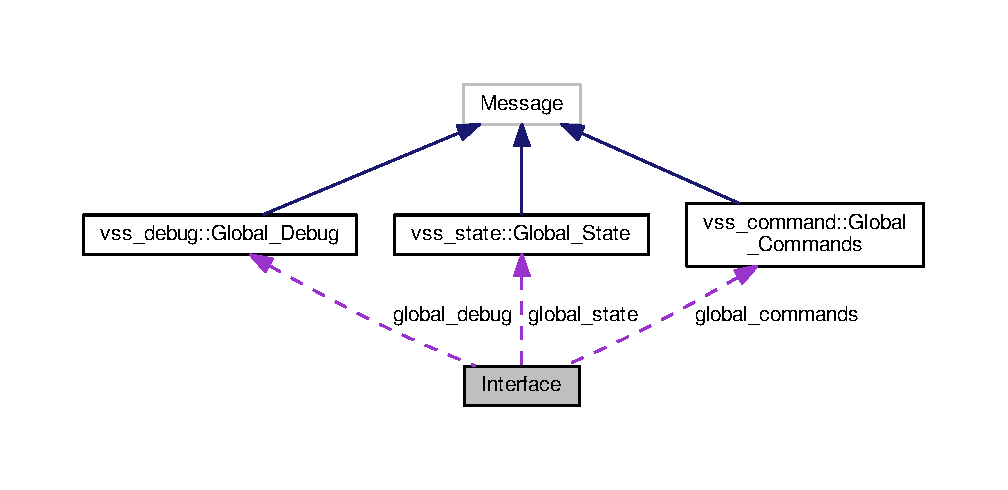
\includegraphics[width=350pt]{classInterface__coll__graph}
\end{center}
\end{figure}
\subsection*{Métodos Públicos}
\begin{DoxyCompactItemize}
\item 
\hyperlink{classInterface_a4406d74c75bdfe150bf72be1f1cda8b1}{Interface} ()\hypertarget{classInterface_a4406d74c75bdfe150bf72be1f1cda8b1}{}\label{classInterface_a4406d74c75bdfe150bf72be1f1cda8b1}

\begin{DoxyCompactList}\small\item\em Construtor D\+E\+F\+A\+U\+LT. \end{DoxyCompactList}\item 
void \hyperlink{classInterface_ac040c88e9847d23f6270a4932527e4d7}{create\+Socket\+Send\+State} (\hyperlink{classvss__state_1_1Global__State}{vss\+\_\+state\+::\+Global\+\_\+\+State} $\ast$, string \hyperlink{classInterface_ae3d7d6a6e2a04ab421b78ebeca7a92c6}{addr\+\_\+server\+\_\+multicast}=\char`\"{}tcp\+://$\ast$\+:5555\char`\"{})
\begin{DoxyCompactList}\small\item\em Método responsável por criar o socket de envio de estados no V\+S\+S-\/\+Vision e V\+S\+S-\/\+Simulator. \end{DoxyCompactList}\item 
void \hyperlink{classInterface_a9de875408d6ec60ef952d167ab244819}{send\+State} ()
\begin{DoxyCompactList}\small\item\em Método respontável por enviar um novo estado pelo V\+S\+S-\/\+Vision e V\+S\+S-\/\+Simulator. \end{DoxyCompactList}\item 
void \hyperlink{classInterface_ac494123d07a83b6e45702f0bfe465acf}{create\+Socket\+Receive\+State} (\hyperlink{classvss__state_1_1Global__State}{vss\+\_\+state\+::\+Global\+\_\+\+State} $\ast$, string \hyperlink{classInterface_af7ac56d5815f432e4b0ba1ae0e55087e}{addr\+\_\+client\+\_\+multicast}=\char`\"{}tcp\+://localhost\+:5555\char`\"{})
\begin{DoxyCompactList}\small\item\em Método responsável por criar o socket de recebimento de estados em V\+S\+S-\/\+Sample\+Strategys. \end{DoxyCompactList}\item 
void \hyperlink{classInterface_abba50a9d10639aa5b2f4a45be31b4062}{receive\+State} ()
\begin{DoxyCompactList}\small\item\em Método responsável por receber um novo estado em V\+S\+S-\/\+Sample\+Strategys. \end{DoxyCompactList}\item 
void \hyperlink{classInterface_af17ffaf827d0090bdbfca933dcb1318a}{create\+Send\+Commands\+Team1} (\hyperlink{classvss__command_1_1Global__Commands}{vss\+\_\+command\+::\+Global\+\_\+\+Commands} $\ast$, string \hyperlink{classInterface_a5fd23546358caf45c28aab623783aa74}{addr\+\_\+client\+\_\+simulator\+\_\+team1}=\char`\"{}tcp\+://localhost\+:5556\char`\"{})
\begin{DoxyCompactList}\small\item\em Método responsável por criar o socket de envio de comandos em V\+S\+S-\/\+Sample\+Strategys ou V\+S\+S-\/\+Joysticks (Time Amarelo) \end{DoxyCompactList}\item 
void \hyperlink{classInterface_af4e4676f7bb5d14c3f1606a9b4ab01e1}{send\+Command\+Team1} ()
\begin{DoxyCompactList}\small\item\em Método responsável por enviar um novo comando por V\+S\+S-\/\+Sample\+Strategys ou V\+S\+S-\/\+Joysticks (Time Amarelo) \end{DoxyCompactList}\item 
void \hyperlink{classInterface_ada4efcce0e1b10c89cea6f24891490ba}{create\+Receive\+Commands\+Team1} (\hyperlink{classvss__command_1_1Global__Commands}{vss\+\_\+command\+::\+Global\+\_\+\+Commands} $\ast$, string \hyperlink{classInterface_afe824e3c6a845f60ef4e95592d6aea8c}{addr\+\_\+server\+\_\+simulator\+\_\+team1}=\char`\"{}tcp\+://$\ast$\+:5556\char`\"{})
\begin{DoxyCompactList}\small\item\em Método responsável por criar o socket de recebimento de comandos no V\+S\+S-\/\+Simulator (Time Amarelo) \end{DoxyCompactList}\item 
void \hyperlink{classInterface_a1e553942adde8b27c3df9dcc1e8cfaa6}{receive\+Command\+Team1} ()
\begin{DoxyCompactList}\small\item\em Método repsonsável por receber um novo comando (Time Amarelo) \end{DoxyCompactList}\item 
void \hyperlink{classInterface_a95658bd3b45221e76f354583b619b9e2}{create\+Send\+Commands\+Team2} (\hyperlink{classvss__command_1_1Global__Commands}{vss\+\_\+command\+::\+Global\+\_\+\+Commands} $\ast$, string \hyperlink{classInterface_a3350d92b68427e361d42e403cd0402ea}{addr\+\_\+client\+\_\+simulator\+\_\+team2}=\char`\"{}tcp\+://localhost\+:5557\char`\"{})
\begin{DoxyCompactList}\small\item\em Método responsável por criar o socket de envio de comandos em V\+S\+S-\/\+Sample\+Strategys ou V\+S\+S-\/\+Joysticks (Time Azul) \end{DoxyCompactList}\item 
void \hyperlink{classInterface_a1c08d024eac24958a1a26d7045288895}{send\+Command\+Team2} ()
\begin{DoxyCompactList}\small\item\em Método responsável por enviar um novo comando por V\+S\+S-\/\+Sample\+Strategys ou V\+S\+S-\/\+Joysticks (Time Azul) \end{DoxyCompactList}\item 
void \hyperlink{classInterface_aac93c76a735e5bacc531472c09c72f07}{create\+Receive\+Commands\+Team2} (\hyperlink{classvss__command_1_1Global__Commands}{vss\+\_\+command\+::\+Global\+\_\+\+Commands} $\ast$, string \hyperlink{classInterface_a5bf42480628d97126c4ccf79dab80608}{addr\+\_\+server\+\_\+simulator\+\_\+team2}=\char`\"{}tcp\+://$\ast$\+:5557\char`\"{})
\begin{DoxyCompactList}\small\item\em Método responsável por criar o socket de recebimento de comandos no V\+S\+S-\/\+Simulator (Time Azul) \end{DoxyCompactList}\item 
void \hyperlink{classInterface_a47c447c89b29ab7e5a9eedc214e2e9cf}{receive\+Command\+Team2} ()
\begin{DoxyCompactList}\small\item\em Método repsonsável por receber um novo comando (Time Azul) \end{DoxyCompactList}\item 
void \hyperlink{classInterface_acf42608b368670e5f8015e343f093934}{create\+Send\+Debug\+Team1} (\hyperlink{classvss__debug_1_1Global__Debug}{vss\+\_\+debug\+::\+Global\+\_\+\+Debug} $\ast$, string \hyperlink{classInterface_a89e46fcba4c30138064e7dfa66520620}{addr\+\_\+client\+\_\+debug\+\_\+team1}=\char`\"{}tcp\+://localhost\+:5558\char`\"{})
\begin{DoxyCompactList}\small\item\em Método responsável por criar o socket de envio de informações de debug em V\+S\+S-\/\+Sample\+Strategys ou V\+S\+S-\/\+Joysticks (Time Amarelo) \end{DoxyCompactList}\item 
void \hyperlink{classInterface_ad3ca9b710198e8f152ceecba608f3ea1}{send\+Debug\+Team1} ()
\begin{DoxyCompactList}\small\item\em Método responsável por enviar uma nova informação de debug por V\+S\+S-\/\+Sample\+Strategys ou V\+S\+S-\/\+Joysticks (Time Amarelo) \end{DoxyCompactList}\item 
void \hyperlink{classInterface_a4b07f8e387443775616852835c78c46d}{create\+Receive\+Debug\+Team1} (\hyperlink{classvss__debug_1_1Global__Debug}{vss\+\_\+debug\+::\+Global\+\_\+\+Debug} $\ast$, string \hyperlink{classInterface_a5e15dc6d237ba5658b621a9267834058}{addr\+\_\+server\+\_\+debug\+\_\+team1}=\char`\"{}tcp\+://$\ast$\+:5558\char`\"{})
\begin{DoxyCompactList}\small\item\em Método responsável por criar o socket de recebimento de informações de debug no V\+S\+S-\/\+Simulator (Time Amarelo) \end{DoxyCompactList}\item 
void \hyperlink{classInterface_a1eaedc1aeabb71b4d7277e7588fdba1b}{receive\+Debug\+Team1} ()
\begin{DoxyCompactList}\small\item\em Método repsonsável por receber uma nova informação de debug (Time Amarelo) \end{DoxyCompactList}\item 
void \hyperlink{classInterface_aef81f08baa4c895699209a4ac884c7c3}{create\+Send\+Debug\+Team2} (\hyperlink{classvss__debug_1_1Global__Debug}{vss\+\_\+debug\+::\+Global\+\_\+\+Debug} $\ast$, string \hyperlink{classInterface_a7c52d0df38af915072bfa3d25539dd74}{addr\+\_\+client\+\_\+debug\+\_\+team2}=\char`\"{}tcp\+://localhost\+:5559\char`\"{})
\begin{DoxyCompactList}\small\item\em Método responsável por criar o socket de envio de informações de debug em V\+S\+S-\/\+Sample\+Strategys ou V\+S\+S-\/\+Joysticks (Time Azul) \end{DoxyCompactList}\item 
void \hyperlink{classInterface_a37b63efacc3c2c0dbaef26cc56c72fd8}{send\+Debug\+Team2} ()
\begin{DoxyCompactList}\small\item\em Método responsável por enviar uma nova informação de debug por V\+S\+S-\/\+Sample\+Strategys ou V\+S\+S-\/\+Joysticks (Time Azul) \end{DoxyCompactList}\item 
void \hyperlink{classInterface_afa3f9885ad6f4ca7f1958d0c578c84b9}{create\+Receive\+Debug\+Team2} (\hyperlink{classvss__debug_1_1Global__Debug}{vss\+\_\+debug\+::\+Global\+\_\+\+Debug} $\ast$, string \hyperlink{classInterface_a4c71300b21d6f2e9cbfdef12cbf01c71}{addr\+\_\+server\+\_\+debug\+\_\+team2}=\char`\"{}tcp\+://$\ast$\+:5559\char`\"{})
\begin{DoxyCompactList}\small\item\em Método responsável por criar o socket de recebimento de informações de debug no V\+S\+S-\/\+Simulator (Time Azul) \end{DoxyCompactList}\item 
void \hyperlink{classInterface_a0e26d81e0b2ace89ac5b9f48481282c6}{receive\+Debug\+Team2} ()
\begin{DoxyCompactList}\small\item\em Método repsonsável por receber uma nova informação de debug (Time Azul) \end{DoxyCompactList}\item 
void \hyperlink{classInterface_ab8f9122465d78b9e41bfde9ea560a657}{print\+State} ()\hypertarget{classInterface_ab8f9122465d78b9e41bfde9ea560a657}{}\label{classInterface_ab8f9122465d78b9e41bfde9ea560a657}

\begin{DoxyCompactList}\small\item\em Método que pode ser utilizado para imprimir o pacote de estado recebido/enviado no terminal. \end{DoxyCompactList}\item 
void \hyperlink{classInterface_aaa4e713b2b72649d5253c83bf9e2416a}{print\+Command} ()\hypertarget{classInterface_aaa4e713b2b72649d5253c83bf9e2416a}{}\label{classInterface_aaa4e713b2b72649d5253c83bf9e2416a}

\begin{DoxyCompactList}\small\item\em Método que pode ser utilizado para imprimir o pacote de comando recebido/enviado no terminal. \end{DoxyCompactList}\item 
void \hyperlink{classInterface_ab7e5653bace447fe9836e8b26ae30247}{print\+Debug} ()\hypertarget{classInterface_ab7e5653bace447fe9836e8b26ae30247}{}\label{classInterface_ab7e5653bace447fe9836e8b26ae30247}

\begin{DoxyCompactList}\small\item\em Método que pode ser utilizado para imprimir o pacote de debug recebido/enviado no terminal. \end{DoxyCompactList}\end{DoxyCompactItemize}
\subsection*{Atributos Protegidos}
\begin{DoxyCompactItemize}
\item 
zmq\+::context\+\_\+t $\ast$ \hyperlink{classInterface_a7a2bda6046550893e9454930636e76d5}{context}\hypertarget{classInterface_a7a2bda6046550893e9454930636e76d5}{}\label{classInterface_a7a2bda6046550893e9454930636e76d5}

\begin{DoxyCompactList}\small\item\em Contexto do socket de envio de estados pelo V\+S\+S-\/\+Vision. E contexto do socket de recebimento de estados pelos V\+S\+S-\/\+Sample\+Strategys. \end{DoxyCompactList}\item 
zmq\+::socket\+\_\+t $\ast$ \hyperlink{classInterface_af38139f534f08df8b3dc9f29001e9584}{socket}\hypertarget{classInterface_af38139f534f08df8b3dc9f29001e9584}{}\label{classInterface_af38139f534f08df8b3dc9f29001e9584}

\begin{DoxyCompactList}\small\item\em Socket de envio de estados pelo V\+S\+S-\/\+Vision. E socket de recebimento de estados pelos V\+S\+S-\/\+Sample\+Strategys. \end{DoxyCompactList}\item 
zmq\+::context\+\_\+t $\ast$ \hyperlink{classInterface_abb1e6fcc090f58ed9f8883584d7bed26}{context\+\_\+command\+\_\+yellow}\hypertarget{classInterface_abb1e6fcc090f58ed9f8883584d7bed26}{}\label{classInterface_abb1e6fcc090f58ed9f8883584d7bed26}

\begin{DoxyCompactList}\small\item\em (Time Amarelo) Contexto do socket de envio de comandos por um V\+S\+S-\/\+Sample\+Strategy ou V\+S\+S-\/\+Joystick. E contexto do socket de recebimento de comandos pelo V\+S\+S-\/\+Simulator \end{DoxyCompactList}\item 
zmq\+::socket\+\_\+t $\ast$ \hyperlink{classInterface_a630819943a79e9f0ce39b7a8147828b5}{socket\+\_\+command\+\_\+yellow}\hypertarget{classInterface_a630819943a79e9f0ce39b7a8147828b5}{}\label{classInterface_a630819943a79e9f0ce39b7a8147828b5}

\begin{DoxyCompactList}\small\item\em (Time Amarelo) Socket de envio de comandos por um V\+S\+S-\/\+Sample\+Strategy ou V\+S\+S-\/\+Joystick. E socket de recebimento de comandos pelo V\+S\+S-\/\+Simulator \end{DoxyCompactList}\item 
zmq\+::context\+\_\+t $\ast$ \hyperlink{classInterface_a3beb279c04dc743f55939597efd85668}{context\+\_\+command\+\_\+blue}\hypertarget{classInterface_a3beb279c04dc743f55939597efd85668}{}\label{classInterface_a3beb279c04dc743f55939597efd85668}

\begin{DoxyCompactList}\small\item\em (Time Azul) Contexto do socket de envio de comandos por um V\+S\+S-\/\+Sample\+Strategy ou V\+S\+S-\/\+Joystick. E contexto do socket de recebimento de comandos pelo V\+S\+S-\/\+Simulator \end{DoxyCompactList}\item 
zmq\+::socket\+\_\+t $\ast$ \hyperlink{classInterface_a2853bd703e1eb4f7ebdb88a21537005f}{socket\+\_\+command\+\_\+blue}\hypertarget{classInterface_a2853bd703e1eb4f7ebdb88a21537005f}{}\label{classInterface_a2853bd703e1eb4f7ebdb88a21537005f}

\begin{DoxyCompactList}\small\item\em (Time Azul) Socket de envio de comandos por um V\+S\+S-\/\+Sample\+Strategy ou V\+S\+S-\/\+Joystick. E socket de recebimento de comandos pelo V\+S\+S-\/\+Simulator \end{DoxyCompactList}\item 
zmq\+::context\+\_\+t $\ast$ \hyperlink{classInterface_ae7b29a3a106e879f2fe60f0176088082}{context\+\_\+debug}\hypertarget{classInterface_ae7b29a3a106e879f2fe60f0176088082}{}\label{classInterface_ae7b29a3a106e879f2fe60f0176088082}

\begin{DoxyCompactList}\small\item\em Contexto do socket de envio de informações de debug por um V\+S\+S-\/\+Sample\+Strategy. E contexto do socket de recebimento de informações de debug pelo V\+S\+S-\/\+Viewer. \end{DoxyCompactList}\item 
zmq\+::socket\+\_\+t $\ast$ \hyperlink{classInterface_a1d7a633715bcdd79ede3ef42e251fcfd}{socket\+\_\+debug}\hypertarget{classInterface_a1d7a633715bcdd79ede3ef42e251fcfd}{}\label{classInterface_a1d7a633715bcdd79ede3ef42e251fcfd}

\begin{DoxyCompactList}\small\item\em Socket de envio de informações de debug por um V\+S\+S-\/\+Sample\+Strategy. E socket de recebimento de informações de debug pelo V\+S\+S-\/\+Viewer. \end{DoxyCompactList}\item 
\hyperlink{classvss__state_1_1Global__State}{vss\+\_\+state\+::\+Global\+\_\+\+State} $\ast$ \hyperlink{classInterface_ac488bcc6708103cb36d132c895efa7a0}{global\+\_\+state}\hypertarget{classInterface_ac488bcc6708103cb36d132c895efa7a0}{}\label{classInterface_ac488bcc6708103cb36d132c895efa7a0}

\begin{DoxyCompactList}\small\item\em Pacote de estados (Utilizado pelo V\+S\+S-\/\+Simulator e V\+S\+S-\/\+Vision, para enviar informações do campo) (Utilizado também pelo V\+S\+S-\/\+Viewer, para desenhar a estado do jogo e pelo V\+S\+S-\/\+Sample\+Strategy para construir-\/se uma estratégia) \end{DoxyCompactList}\item 
\hyperlink{classvss__command_1_1Global__Commands}{vss\+\_\+command\+::\+Global\+\_\+\+Commands} $\ast$ \hyperlink{classInterface_a0109a54da68b3e7cd0c652f6cdd75abe}{global\+\_\+commands}\hypertarget{classInterface_a0109a54da68b3e7cd0c652f6cdd75abe}{}\label{classInterface_a0109a54da68b3e7cd0c652f6cdd75abe}

\begin{DoxyCompactList}\small\item\em Pacote de comandos (Utilizado por V\+S\+S-\/\+Sample\+Strategys e V\+S\+S-\/\+Joysticks, para enviar comandos para robôs virtuais) (Utilizado também pelo V\+S\+S-\/\+Simulator, para receber os comandos de cada robô) \end{DoxyCompactList}\item 
\hyperlink{classvss__debug_1_1Global__Debug}{vss\+\_\+debug\+::\+Global\+\_\+\+Debug} $\ast$ \hyperlink{classInterface_a2601489a867659e158bbff1bd2470411}{global\+\_\+debug}\hypertarget{classInterface_a2601489a867659e158bbff1bd2470411}{}\label{classInterface_a2601489a867659e158bbff1bd2470411}

\begin{DoxyCompactList}\small\item\em Pacote de debug visual (Utilizado por V\+S\+S-\/\+Sample\+Strategys, para enviar informações da estratégia para o V\+S\+S-\/\+Viewer desenhar) \end{DoxyCompactList}\item 
string \hyperlink{classInterface_ae3d7d6a6e2a04ab421b78ebeca7a92c6}{addr\+\_\+server\+\_\+multicast}\hypertarget{classInterface_ae3d7d6a6e2a04ab421b78ebeca7a92c6}{}\label{classInterface_ae3d7d6a6e2a04ab421b78ebeca7a92c6}

\begin{DoxyCompactList}\small\item\em Endereço multicast do envio de estados por parte do V\+S\+S-\/\+Simulator e V\+S\+S-\/\+Vision (V\+S\+S-\/\+Vision e V\+S\+S-\/\+Simulator não podem ser abertos ao mesmo tempo) \end{DoxyCompactList}\item 
string \hyperlink{classInterface_af7ac56d5815f432e4b0ba1ae0e55087e}{addr\+\_\+client\+\_\+multicast}\hypertarget{classInterface_af7ac56d5815f432e4b0ba1ae0e55087e}{}\label{classInterface_af7ac56d5815f432e4b0ba1ae0e55087e}

\begin{DoxyCompactList}\small\item\em Endereço mulsticast do recebimento dos estados por parte do V\+S\+S-\/\+Viewer e V\+S\+S-\/\+Sample\+Strategys. \end{DoxyCompactList}\item 
string \hyperlink{classInterface_afe824e3c6a845f60ef4e95592d6aea8c}{addr\+\_\+server\+\_\+simulator\+\_\+team1}\hypertarget{classInterface_afe824e3c6a845f60ef4e95592d6aea8c}{}\label{classInterface_afe824e3c6a845f60ef4e95592d6aea8c}

\begin{DoxyCompactList}\small\item\em (Time Amarelo) Endereço unicast para recebimento dessas informações pelo V\+S\+S-\/\+Simulator \end{DoxyCompactList}\item 
string \hyperlink{classInterface_a5fd23546358caf45c28aab623783aa74}{addr\+\_\+client\+\_\+simulator\+\_\+team1}\hypertarget{classInterface_a5fd23546358caf45c28aab623783aa74}{}\label{classInterface_a5fd23546358caf45c28aab623783aa74}

\begin{DoxyCompactList}\small\item\em (Time Amarelo) Endereço unicast para envio de comandos por V\+S\+S-\/\+Sample\+Strategys ou V\+S\+S-\/\+Joysticks \end{DoxyCompactList}\item 
string \hyperlink{classInterface_a5bf42480628d97126c4ccf79dab80608}{addr\+\_\+server\+\_\+simulator\+\_\+team2}\hypertarget{classInterface_a5bf42480628d97126c4ccf79dab80608}{}\label{classInterface_a5bf42480628d97126c4ccf79dab80608}

\begin{DoxyCompactList}\small\item\em (Time Azul) Endereços unicast para recebimento dessas informações pelo V\+S\+S-\/\+Simulator \end{DoxyCompactList}\item 
string \hyperlink{classInterface_a3350d92b68427e361d42e403cd0402ea}{addr\+\_\+client\+\_\+simulator\+\_\+team2}\hypertarget{classInterface_a3350d92b68427e361d42e403cd0402ea}{}\label{classInterface_a3350d92b68427e361d42e403cd0402ea}

\begin{DoxyCompactList}\small\item\em (Time Azul) Endereços unicast para envio de comandos por V\+S\+S-\/\+Sample\+Strategys ou V\+S\+S-\/\+Joysticks \end{DoxyCompactList}\item 
string \hyperlink{classInterface_a5e15dc6d237ba5658b621a9267834058}{addr\+\_\+server\+\_\+debug\+\_\+team1}\hypertarget{classInterface_a5e15dc6d237ba5658b621a9267834058}{}\label{classInterface_a5e15dc6d237ba5658b621a9267834058}

\begin{DoxyCompactList}\small\item\em (Time Amarelo) Endereço unicast para recebimento de informações de debug pelo V\+S\+S-\/\+Viewer \end{DoxyCompactList}\item 
string \hyperlink{classInterface_a89e46fcba4c30138064e7dfa66520620}{addr\+\_\+client\+\_\+debug\+\_\+team1}\hypertarget{classInterface_a89e46fcba4c30138064e7dfa66520620}{}\label{classInterface_a89e46fcba4c30138064e7dfa66520620}

\begin{DoxyCompactList}\small\item\em (Time Amarelo) Endereço unicast para envio de informações de debug por V\+S\+S-\/\+Sample\+Strategys \end{DoxyCompactList}\item 
string \hyperlink{classInterface_a4c71300b21d6f2e9cbfdef12cbf01c71}{addr\+\_\+server\+\_\+debug\+\_\+team2}\hypertarget{classInterface_a4c71300b21d6f2e9cbfdef12cbf01c71}{}\label{classInterface_a4c71300b21d6f2e9cbfdef12cbf01c71}

\begin{DoxyCompactList}\small\item\em (Time Azul) Endereço unicast para recebimento de informações de debug pelo V\+S\+S-\/\+Viewer \end{DoxyCompactList}\item 
string \hyperlink{classInterface_a7c52d0df38af915072bfa3d25539dd74}{addr\+\_\+client\+\_\+debug\+\_\+team2}\hypertarget{classInterface_a7c52d0df38af915072bfa3d25539dd74}{}\label{classInterface_a7c52d0df38af915072bfa3d25539dd74}

\begin{DoxyCompactList}\small\item\em (Time Azul) Endereço unicast para envio de informações de debug por V\+S\+S-\/\+Sample\+Strategys \end{DoxyCompactList}\end{DoxyCompactItemize}


\subsection{Descrição Detalhada}
Essa classe define as interfaces utilizadas em todos os projetos do V\+S\+S-\/\+S\+DK, em outras palavras, todos os sockets abertos em todos os projetos estão aqui. 

\subsection{Métodos}
\index{Interface@{Interface}!create\+Receive\+Commands\+Team1@{create\+Receive\+Commands\+Team1}}
\index{create\+Receive\+Commands\+Team1@{create\+Receive\+Commands\+Team1}!Interface@{Interface}}
\subsubsection[{\texorpdfstring{create\+Receive\+Commands\+Team1(vss\+\_\+command\+::\+Global\+\_\+\+Commands $\ast$, string addr\+\_\+server\+\_\+simulator\+\_\+team1=""tcp\+://$\ast$\+:5556"")}{createReceiveCommandsTeam1(vss_command::Global_Commands *, string addr_server_simulator_team1="tcp://*:5556")}}]{\setlength{\rightskip}{0pt plus 5cm}void Interface\+::create\+Receive\+Commands\+Team1 (
\begin{DoxyParamCaption}
\item[{{\bf vss\+\_\+command\+::\+Global\+\_\+\+Commands} $\ast$}]{global\+\_\+commands, }
\item[{string}]{addr\+\_\+server\+\_\+simulator\+\_\+team1 = {\ttfamily \char`\"{}tcp\+://$\ast$\+:5556\char`\"{}}}
\end{DoxyParamCaption}
)}\hypertarget{classInterface_ada4efcce0e1b10c89cea6f24891490ba}{}\label{classInterface_ada4efcce0e1b10c89cea6f24891490ba}


Método responsável por criar o socket de recebimento de comandos no V\+S\+S-\/\+Simulator (Time Amarelo) 

Esse método deve ser chamado apenas uma vez. Global\+\_\+\+Commands é recebido como ponteiro, assim facilitando o recebimento de novos comandos \index{Interface@{Interface}!create\+Receive\+Commands\+Team2@{create\+Receive\+Commands\+Team2}}
\index{create\+Receive\+Commands\+Team2@{create\+Receive\+Commands\+Team2}!Interface@{Interface}}
\subsubsection[{\texorpdfstring{create\+Receive\+Commands\+Team2(vss\+\_\+command\+::\+Global\+\_\+\+Commands $\ast$, string addr\+\_\+server\+\_\+simulator\+\_\+team2=""tcp\+://$\ast$\+:5557"")}{createReceiveCommandsTeam2(vss_command::Global_Commands *, string addr_server_simulator_team2="tcp://*:5557")}}]{\setlength{\rightskip}{0pt plus 5cm}void Interface\+::create\+Receive\+Commands\+Team2 (
\begin{DoxyParamCaption}
\item[{{\bf vss\+\_\+command\+::\+Global\+\_\+\+Commands} $\ast$}]{global\+\_\+commands, }
\item[{string}]{addr\+\_\+server\+\_\+simulator\+\_\+team2 = {\ttfamily \char`\"{}tcp\+://$\ast$\+:5557\char`\"{}}}
\end{DoxyParamCaption}
)}\hypertarget{classInterface_aac93c76a735e5bacc531472c09c72f07}{}\label{classInterface_aac93c76a735e5bacc531472c09c72f07}


Método responsável por criar o socket de recebimento de comandos no V\+S\+S-\/\+Simulator (Time Azul) 

Esse método deve ser chamado apenas uma vez. Global\+\_\+\+Commands é recebido como ponteiro, assim facilitando o envio de novos comandos \index{Interface@{Interface}!create\+Receive\+Debug\+Team1@{create\+Receive\+Debug\+Team1}}
\index{create\+Receive\+Debug\+Team1@{create\+Receive\+Debug\+Team1}!Interface@{Interface}}
\subsubsection[{\texorpdfstring{create\+Receive\+Debug\+Team1(vss\+\_\+debug\+::\+Global\+\_\+\+Debug $\ast$, string addr\+\_\+server\+\_\+debug\+\_\+team1=""tcp\+://$\ast$\+:5558"")}{createReceiveDebugTeam1(vss_debug::Global_Debug *, string addr_server_debug_team1="tcp://*:5558")}}]{\setlength{\rightskip}{0pt plus 5cm}void Interface\+::create\+Receive\+Debug\+Team1 (
\begin{DoxyParamCaption}
\item[{{\bf vss\+\_\+debug\+::\+Global\+\_\+\+Debug} $\ast$}]{global\+\_\+debug, }
\item[{string}]{addr\+\_\+server\+\_\+debug\+\_\+team1 = {\ttfamily \char`\"{}tcp\+://$\ast$\+:5558\char`\"{}}}
\end{DoxyParamCaption}
)}\hypertarget{classInterface_a4b07f8e387443775616852835c78c46d}{}\label{classInterface_a4b07f8e387443775616852835c78c46d}


Método responsável por criar o socket de recebimento de informações de debug no V\+S\+S-\/\+Simulator (Time Amarelo) 

Esse método deve ser chamado apenas uma vez. Global\+\_\+\+Debug é recebido como ponteiro, assim facilitando o recebimento de novas informações de debug \index{Interface@{Interface}!create\+Receive\+Debug\+Team2@{create\+Receive\+Debug\+Team2}}
\index{create\+Receive\+Debug\+Team2@{create\+Receive\+Debug\+Team2}!Interface@{Interface}}
\subsubsection[{\texorpdfstring{create\+Receive\+Debug\+Team2(vss\+\_\+debug\+::\+Global\+\_\+\+Debug $\ast$, string addr\+\_\+server\+\_\+debug\+\_\+team2=""tcp\+://$\ast$\+:5559"")}{createReceiveDebugTeam2(vss_debug::Global_Debug *, string addr_server_debug_team2="tcp://*:5559")}}]{\setlength{\rightskip}{0pt plus 5cm}void Interface\+::create\+Receive\+Debug\+Team2 (
\begin{DoxyParamCaption}
\item[{{\bf vss\+\_\+debug\+::\+Global\+\_\+\+Debug} $\ast$}]{global\+\_\+debug, }
\item[{string}]{addr\+\_\+server\+\_\+debug\+\_\+team2 = {\ttfamily \char`\"{}tcp\+://$\ast$\+:5559\char`\"{}}}
\end{DoxyParamCaption}
)}\hypertarget{classInterface_afa3f9885ad6f4ca7f1958d0c578c84b9}{}\label{classInterface_afa3f9885ad6f4ca7f1958d0c578c84b9}


Método responsável por criar o socket de recebimento de informações de debug no V\+S\+S-\/\+Simulator (Time Azul) 

Esse método deve ser chamado apenas uma vez. Global\+\_\+\+Debug é recebido como ponteiro, assim facilitando o recebimento de novas informações de debug \index{Interface@{Interface}!create\+Send\+Commands\+Team1@{create\+Send\+Commands\+Team1}}
\index{create\+Send\+Commands\+Team1@{create\+Send\+Commands\+Team1}!Interface@{Interface}}
\subsubsection[{\texorpdfstring{create\+Send\+Commands\+Team1(vss\+\_\+command\+::\+Global\+\_\+\+Commands $\ast$, string addr\+\_\+client\+\_\+simulator\+\_\+team1=""tcp\+://localhost\+:5556"")}{createSendCommandsTeam1(vss_command::Global_Commands *, string addr_client_simulator_team1="tcp://localhost:5556")}}]{\setlength{\rightskip}{0pt plus 5cm}void Interface\+::create\+Send\+Commands\+Team1 (
\begin{DoxyParamCaption}
\item[{{\bf vss\+\_\+command\+::\+Global\+\_\+\+Commands} $\ast$}]{global\+\_\+commands, }
\item[{string}]{addr\+\_\+client\+\_\+simulator\+\_\+team1 = {\ttfamily \char`\"{}tcp\+://localhost\+:5556\char`\"{}}}
\end{DoxyParamCaption}
)}\hypertarget{classInterface_af17ffaf827d0090bdbfca933dcb1318a}{}\label{classInterface_af17ffaf827d0090bdbfca933dcb1318a}


Método responsável por criar o socket de envio de comandos em V\+S\+S-\/\+Sample\+Strategys ou V\+S\+S-\/\+Joysticks (Time Amarelo) 

Esse método deve ser chamado apenas uma vez. Global\+\_\+\+Commands é recebido como ponteiro, assim facilitando o envio de novos comandos \index{Interface@{Interface}!create\+Send\+Commands\+Team2@{create\+Send\+Commands\+Team2}}
\index{create\+Send\+Commands\+Team2@{create\+Send\+Commands\+Team2}!Interface@{Interface}}
\subsubsection[{\texorpdfstring{create\+Send\+Commands\+Team2(vss\+\_\+command\+::\+Global\+\_\+\+Commands $\ast$, string addr\+\_\+client\+\_\+simulator\+\_\+team2=""tcp\+://localhost\+:5557"")}{createSendCommandsTeam2(vss_command::Global_Commands *, string addr_client_simulator_team2="tcp://localhost:5557")}}]{\setlength{\rightskip}{0pt plus 5cm}void Interface\+::create\+Send\+Commands\+Team2 (
\begin{DoxyParamCaption}
\item[{{\bf vss\+\_\+command\+::\+Global\+\_\+\+Commands} $\ast$}]{global\+\_\+commands, }
\item[{string}]{addr\+\_\+client\+\_\+simulator\+\_\+team2 = {\ttfamily \char`\"{}tcp\+://localhost\+:5557\char`\"{}}}
\end{DoxyParamCaption}
)}\hypertarget{classInterface_a95658bd3b45221e76f354583b619b9e2}{}\label{classInterface_a95658bd3b45221e76f354583b619b9e2}


Método responsável por criar o socket de envio de comandos em V\+S\+S-\/\+Sample\+Strategys ou V\+S\+S-\/\+Joysticks (Time Azul) 

Esse método deve ser chamado apenas uma vez. Global\+\_\+\+Commands é recebido como ponteiro, assim facilitando o envio de novos comandos \index{Interface@{Interface}!create\+Send\+Debug\+Team1@{create\+Send\+Debug\+Team1}}
\index{create\+Send\+Debug\+Team1@{create\+Send\+Debug\+Team1}!Interface@{Interface}}
\subsubsection[{\texorpdfstring{create\+Send\+Debug\+Team1(vss\+\_\+debug\+::\+Global\+\_\+\+Debug $\ast$, string addr\+\_\+client\+\_\+debug\+\_\+team1=""tcp\+://localhost\+:5558"")}{createSendDebugTeam1(vss_debug::Global_Debug *, string addr_client_debug_team1="tcp://localhost:5558")}}]{\setlength{\rightskip}{0pt plus 5cm}void Interface\+::create\+Send\+Debug\+Team1 (
\begin{DoxyParamCaption}
\item[{{\bf vss\+\_\+debug\+::\+Global\+\_\+\+Debug} $\ast$}]{global\+\_\+debug, }
\item[{string}]{addr\+\_\+client\+\_\+debug\+\_\+team1 = {\ttfamily \char`\"{}tcp\+://localhost\+:5558\char`\"{}}}
\end{DoxyParamCaption}
)}\hypertarget{classInterface_acf42608b368670e5f8015e343f093934}{}\label{classInterface_acf42608b368670e5f8015e343f093934}


Método responsável por criar o socket de envio de informações de debug em V\+S\+S-\/\+Sample\+Strategys ou V\+S\+S-\/\+Joysticks (Time Amarelo) 

Esse método deve ser chamado apenas uma vez. Global\+\_\+\+Debug é recebido como ponteiro, assim facilitando o envio de novas informações de debug \index{Interface@{Interface}!create\+Send\+Debug\+Team2@{create\+Send\+Debug\+Team2}}
\index{create\+Send\+Debug\+Team2@{create\+Send\+Debug\+Team2}!Interface@{Interface}}
\subsubsection[{\texorpdfstring{create\+Send\+Debug\+Team2(vss\+\_\+debug\+::\+Global\+\_\+\+Debug $\ast$, string addr\+\_\+client\+\_\+debug\+\_\+team2=""tcp\+://localhost\+:5559"")}{createSendDebugTeam2(vss_debug::Global_Debug *, string addr_client_debug_team2="tcp://localhost:5559")}}]{\setlength{\rightskip}{0pt plus 5cm}void Interface\+::create\+Send\+Debug\+Team2 (
\begin{DoxyParamCaption}
\item[{{\bf vss\+\_\+debug\+::\+Global\+\_\+\+Debug} $\ast$}]{global\+\_\+debug, }
\item[{string}]{addr\+\_\+client\+\_\+debug\+\_\+team2 = {\ttfamily \char`\"{}tcp\+://localhost\+:5559\char`\"{}}}
\end{DoxyParamCaption}
)}\hypertarget{classInterface_aef81f08baa4c895699209a4ac884c7c3}{}\label{classInterface_aef81f08baa4c895699209a4ac884c7c3}


Método responsável por criar o socket de envio de informações de debug em V\+S\+S-\/\+Sample\+Strategys ou V\+S\+S-\/\+Joysticks (Time Azul) 

Esse método deve ser chamado apenas uma vez. Global\+\_\+\+Debug é recebido como ponteiro, assim facilitando o envio de novas informações de debug \index{Interface@{Interface}!create\+Socket\+Receive\+State@{create\+Socket\+Receive\+State}}
\index{create\+Socket\+Receive\+State@{create\+Socket\+Receive\+State}!Interface@{Interface}}
\subsubsection[{\texorpdfstring{create\+Socket\+Receive\+State(vss\+\_\+state\+::\+Global\+\_\+\+State $\ast$, string addr\+\_\+client\+\_\+multicast=""tcp\+://localhost\+:5555"")}{createSocketReceiveState(vss_state::Global_State *, string addr_client_multicast="tcp://localhost:5555")}}]{\setlength{\rightskip}{0pt plus 5cm}void Interface\+::create\+Socket\+Receive\+State (
\begin{DoxyParamCaption}
\item[{{\bf vss\+\_\+state\+::\+Global\+\_\+\+State} $\ast$}]{global\+\_\+state, }
\item[{string}]{addr\+\_\+client\+\_\+multicast = {\ttfamily \char`\"{}tcp\+://localhost\+:5555\char`\"{}}}
\end{DoxyParamCaption}
)}\hypertarget{classInterface_ac494123d07a83b6e45702f0bfe465acf}{}\label{classInterface_ac494123d07a83b6e45702f0bfe465acf}


Método responsável por criar o socket de recebimento de estados em V\+S\+S-\/\+Sample\+Strategys. 

Esse método deve ser chamado apenas uma vez. Global\+\_\+\+State é recebido como ponteiro, assim facilitando o recebimento de novos estados \index{Interface@{Interface}!create\+Socket\+Send\+State@{create\+Socket\+Send\+State}}
\index{create\+Socket\+Send\+State@{create\+Socket\+Send\+State}!Interface@{Interface}}
\subsubsection[{\texorpdfstring{create\+Socket\+Send\+State(vss\+\_\+state\+::\+Global\+\_\+\+State $\ast$, string addr\+\_\+server\+\_\+multicast=""tcp\+://$\ast$\+:5555"")}{createSocketSendState(vss_state::Global_State *, string addr_server_multicast="tcp://*:5555")}}]{\setlength{\rightskip}{0pt plus 5cm}void Interface\+::create\+Socket\+Send\+State (
\begin{DoxyParamCaption}
\item[{{\bf vss\+\_\+state\+::\+Global\+\_\+\+State} $\ast$}]{global\+\_\+state, }
\item[{string}]{addr\+\_\+server\+\_\+multicast = {\ttfamily \char`\"{}tcp\+://$\ast$\+:5555\char`\"{}}}
\end{DoxyParamCaption}
)}\hypertarget{classInterface_ac040c88e9847d23f6270a4932527e4d7}{}\label{classInterface_ac040c88e9847d23f6270a4932527e4d7}


Método responsável por criar o socket de envio de estados no V\+S\+S-\/\+Vision e V\+S\+S-\/\+Simulator. 

Esse método deve ser chamado apenas uma vez. Global\+\_\+\+State é recebido como ponteiro, assim facilitando o envio de novos estados \index{Interface@{Interface}!receive\+Command\+Team1@{receive\+Command\+Team1}}
\index{receive\+Command\+Team1@{receive\+Command\+Team1}!Interface@{Interface}}
\subsubsection[{\texorpdfstring{receive\+Command\+Team1()}{receiveCommandTeam1()}}]{\setlength{\rightskip}{0pt plus 5cm}void Interface\+::receive\+Command\+Team1 (
\begin{DoxyParamCaption}
{}
\end{DoxyParamCaption}
)}\hypertarget{classInterface_a1e553942adde8b27c3df9dcc1e8cfaa6}{}\label{classInterface_a1e553942adde8b27c3df9dcc1e8cfaa6}


Método repsonsável por receber um novo comando (Time Amarelo) 

Esse método deve ser chamado em um loop infinito controlado. O recebimento tratado aqui é bloqueante Chamando esse método, o Global\+\_\+\+Commands passado por ponteiro na construção do socket automaticamente é atualizado \index{Interface@{Interface}!receive\+Command\+Team2@{receive\+Command\+Team2}}
\index{receive\+Command\+Team2@{receive\+Command\+Team2}!Interface@{Interface}}
\subsubsection[{\texorpdfstring{receive\+Command\+Team2()}{receiveCommandTeam2()}}]{\setlength{\rightskip}{0pt plus 5cm}void Interface\+::receive\+Command\+Team2 (
\begin{DoxyParamCaption}
{}
\end{DoxyParamCaption}
)}\hypertarget{classInterface_a47c447c89b29ab7e5a9eedc214e2e9cf}{}\label{classInterface_a47c447c89b29ab7e5a9eedc214e2e9cf}


Método repsonsável por receber um novo comando (Time Azul) 

Esse método deve ser chamado em um loop infinito controlado. O recebimento tratado aqui é bloqueante Chamando esse método, o Global\+\_\+\+Commands passado por ponteiro na construção do socket automaticamente é atualizado \index{Interface@{Interface}!receive\+Debug\+Team1@{receive\+Debug\+Team1}}
\index{receive\+Debug\+Team1@{receive\+Debug\+Team1}!Interface@{Interface}}
\subsubsection[{\texorpdfstring{receive\+Debug\+Team1()}{receiveDebugTeam1()}}]{\setlength{\rightskip}{0pt plus 5cm}void Interface\+::receive\+Debug\+Team1 (
\begin{DoxyParamCaption}
{}
\end{DoxyParamCaption}
)}\hypertarget{classInterface_a1eaedc1aeabb71b4d7277e7588fdba1b}{}\label{classInterface_a1eaedc1aeabb71b4d7277e7588fdba1b}


Método repsonsável por receber uma nova informação de debug (Time Amarelo) 

Esse método deve ser chamado em um loop infinito controlado. O recebimento tratado aqui é bloqueante Chamando esse método, o Global\+\_\+\+Debug passado por ponteiro na construção do socket automaticamente é atualizado \index{Interface@{Interface}!receive\+Debug\+Team2@{receive\+Debug\+Team2}}
\index{receive\+Debug\+Team2@{receive\+Debug\+Team2}!Interface@{Interface}}
\subsubsection[{\texorpdfstring{receive\+Debug\+Team2()}{receiveDebugTeam2()}}]{\setlength{\rightskip}{0pt plus 5cm}void Interface\+::receive\+Debug\+Team2 (
\begin{DoxyParamCaption}
{}
\end{DoxyParamCaption}
)}\hypertarget{classInterface_a0e26d81e0b2ace89ac5b9f48481282c6}{}\label{classInterface_a0e26d81e0b2ace89ac5b9f48481282c6}


Método repsonsável por receber uma nova informação de debug (Time Azul) 

Esse método deve ser chamado em um loop infinito controlado. O recebimento tratado aqui é bloqueante Chamando esse método, o Global\+\_\+\+Debug passado por ponteiro na construção do socket automaticamente é atualizado \index{Interface@{Interface}!receive\+State@{receive\+State}}
\index{receive\+State@{receive\+State}!Interface@{Interface}}
\subsubsection[{\texorpdfstring{receive\+State()}{receiveState()}}]{\setlength{\rightskip}{0pt plus 5cm}void Interface\+::receive\+State (
\begin{DoxyParamCaption}
{}
\end{DoxyParamCaption}
)}\hypertarget{classInterface_abba50a9d10639aa5b2f4a45be31b4062}{}\label{classInterface_abba50a9d10639aa5b2f4a45be31b4062}


Método responsável por receber um novo estado em V\+S\+S-\/\+Sample\+Strategys. 

Esse método deve ser chamado em um loop infinito controlado. O recebimento tratado aqui é não bloqueante Chamando esse método, o Global\+\_\+\+State passado por ponteiro na construção do socket automaticamente é atualizado \index{Interface@{Interface}!send\+Command\+Team1@{send\+Command\+Team1}}
\index{send\+Command\+Team1@{send\+Command\+Team1}!Interface@{Interface}}
\subsubsection[{\texorpdfstring{send\+Command\+Team1()}{sendCommandTeam1()}}]{\setlength{\rightskip}{0pt plus 5cm}void Interface\+::send\+Command\+Team1 (
\begin{DoxyParamCaption}
{}
\end{DoxyParamCaption}
)}\hypertarget{classInterface_af4e4676f7bb5d14c3f1606a9b4ab01e1}{}\label{classInterface_af4e4676f7bb5d14c3f1606a9b4ab01e1}


Método responsável por enviar um novo comando por V\+S\+S-\/\+Sample\+Strategys ou V\+S\+S-\/\+Joysticks (Time Amarelo) 

Esse método deve ser chamado em um loop infinito controlado. O envio tratado aqui é bloqueante Chamando esse método, o Global\+\_\+\+Commands passado por ponteiro na construção do socket automaticamente é atualizado \index{Interface@{Interface}!send\+Command\+Team2@{send\+Command\+Team2}}
\index{send\+Command\+Team2@{send\+Command\+Team2}!Interface@{Interface}}
\subsubsection[{\texorpdfstring{send\+Command\+Team2()}{sendCommandTeam2()}}]{\setlength{\rightskip}{0pt plus 5cm}void Interface\+::send\+Command\+Team2 (
\begin{DoxyParamCaption}
{}
\end{DoxyParamCaption}
)}\hypertarget{classInterface_a1c08d024eac24958a1a26d7045288895}{}\label{classInterface_a1c08d024eac24958a1a26d7045288895}


Método responsável por enviar um novo comando por V\+S\+S-\/\+Sample\+Strategys ou V\+S\+S-\/\+Joysticks (Time Azul) 

Esse método deve ser chamado em um loop infinito controlado. O envio tratado aqui é bloqueante Chamando esse método, o Global\+\_\+\+Commands passado por ponteiro na construção do socket automaticamente é atualizado \index{Interface@{Interface}!send\+Debug\+Team1@{send\+Debug\+Team1}}
\index{send\+Debug\+Team1@{send\+Debug\+Team1}!Interface@{Interface}}
\subsubsection[{\texorpdfstring{send\+Debug\+Team1()}{sendDebugTeam1()}}]{\setlength{\rightskip}{0pt plus 5cm}void Interface\+::send\+Debug\+Team1 (
\begin{DoxyParamCaption}
{}
\end{DoxyParamCaption}
)}\hypertarget{classInterface_ad3ca9b710198e8f152ceecba608f3ea1}{}\label{classInterface_ad3ca9b710198e8f152ceecba608f3ea1}


Método responsável por enviar uma nova informação de debug por V\+S\+S-\/\+Sample\+Strategys ou V\+S\+S-\/\+Joysticks (Time Amarelo) 

Esse método deve ser chamado em um loop infinito controlado. O envio tratado aqui é bloqueante Chamando esse método, o Global\+\_\+\+Debug passado por ponteiro na construção do socket automaticamente é atualizado \index{Interface@{Interface}!send\+Debug\+Team2@{send\+Debug\+Team2}}
\index{send\+Debug\+Team2@{send\+Debug\+Team2}!Interface@{Interface}}
\subsubsection[{\texorpdfstring{send\+Debug\+Team2()}{sendDebugTeam2()}}]{\setlength{\rightskip}{0pt plus 5cm}void Interface\+::send\+Debug\+Team2 (
\begin{DoxyParamCaption}
{}
\end{DoxyParamCaption}
)}\hypertarget{classInterface_a37b63efacc3c2c0dbaef26cc56c72fd8}{}\label{classInterface_a37b63efacc3c2c0dbaef26cc56c72fd8}


Método responsável por enviar uma nova informação de debug por V\+S\+S-\/\+Sample\+Strategys ou V\+S\+S-\/\+Joysticks (Time Azul) 

Esse método deve ser chamado em um loop infinito controlado. O envio tratado aqui é bloqueante Chamando esse método, o Global\+\_\+\+Debug passado por ponteiro na construção do socket automaticamente é atualizado \index{Interface@{Interface}!send\+State@{send\+State}}
\index{send\+State@{send\+State}!Interface@{Interface}}
\subsubsection[{\texorpdfstring{send\+State()}{sendState()}}]{\setlength{\rightskip}{0pt plus 5cm}void Interface\+::send\+State (
\begin{DoxyParamCaption}
{}
\end{DoxyParamCaption}
)}\hypertarget{classInterface_a9de875408d6ec60ef952d167ab244819}{}\label{classInterface_a9de875408d6ec60ef952d167ab244819}


Método respontável por enviar um novo estado pelo V\+S\+S-\/\+Vision e V\+S\+S-\/\+Simulator. 

Esse método deve ser chamado em um loop infinito controlado. O envio tratado aqui é não bloqueante Chamando esse método, o Global\+\_\+\+State passado por ponteiro na construção do socket automaticamente é atualizado 

A documentação para esta classe foi gerada a partir dos seguintes arquivos\+:\begin{DoxyCompactItemize}
\item 
/home/johnathan/\+Repositories/\+S\+I\+R\+Lab/\+Public/\+V\+S\+S-\/\+Viewer/src/\+V\+S\+S-\/\+Interface/interface.\+h\item 
/home/johnathan/\+Repositories/\+S\+I\+R\+Lab/\+Public/\+V\+S\+S-\/\+Viewer/src/\+V\+S\+S-\/\+Interface/interface.\+cpp\end{DoxyCompactItemize}

\hypertarget{structcommon_1_1Path}{}\section{Referência da Estrutura common\+:\+:Path}
\label{structcommon_1_1Path}\index{common\+::\+Path@{common\+::\+Path}}


Essa struct é responsável por representar um caminho.  




{\ttfamily \#include $<$commons.\+h$>$}

\subsection*{Métodos Públicos}
\begin{DoxyCompactItemize}
\item 
\hyperlink{structcommon_1_1Path_aa594e5d456d0ec2357d302cb5c898043}{Path} ()\hypertarget{structcommon_1_1Path_aa594e5d456d0ec2357d302cb5c898043}{}\label{structcommon_1_1Path_aa594e5d456d0ec2357d302cb5c898043}

\begin{DoxyCompactList}\small\item\em Construtor D\+E\+F\+A\+U\+LT. \end{DoxyCompactList}\item 
\hyperlink{structcommon_1_1Path_adc2653fd1a8605ddef65cb96c814b423}{Path} (\hyperlink{structcommon_1_1Path}{Path} $\ast$path)\hypertarget{structcommon_1_1Path_adc2653fd1a8605ddef65cb96c814b423}{}\label{structcommon_1_1Path_adc2653fd1a8605ddef65cb96c814b423}

\begin{DoxyCompactList}\small\item\em Construtor cópia. \end{DoxyCompactList}\item 
void \hyperlink{structcommon_1_1Path_a1258d2f94073ac9d2995617ff7d2ac46}{show} ()\hypertarget{structcommon_1_1Path_a1258d2f94073ac9d2995617ff7d2ac46}{}\label{structcommon_1_1Path_a1258d2f94073ac9d2995617ff7d2ac46}

\begin{DoxyCompactList}\small\item\em Método de debug no terminal. \end{DoxyCompactList}\end{DoxyCompactItemize}
\subsection*{Atributos Públicos}
\begin{DoxyCompactItemize}
\item 
vector$<$ \hyperlink{structcommon_1_1Pose}{Pose} $>$ \hyperlink{structcommon_1_1Path_ad6561127227344b7c0a24c04dc05cbd4}{poses}\hypertarget{structcommon_1_1Path_ad6561127227344b7c0a24c04dc05cbd4}{}\label{structcommon_1_1Path_ad6561127227344b7c0a24c04dc05cbd4}

\begin{DoxyCompactList}\small\item\em Um caminho é tido como uma sequência de poses. \end{DoxyCompactList}\end{DoxyCompactItemize}


\subsection{Descrição Detalhada}
Essa struct é responsável por representar um caminho. 

A documentação para esta estrutura foi gerada a partir do seguinte arquivo\+:\begin{DoxyCompactItemize}
\item 
/home/johnathan/\+Repositories/\+S\+I\+R\+Lab/\+Projects/\+V\+S\+S-\/\+Viewer/src/commons.\+h\end{DoxyCompactItemize}

\hypertarget{classvss__debug_1_1Path}{}\section{Referência da Classe vss\+\_\+debug\+:\+:Path}
\label{classvss__debug_1_1Path}\index{vss\+\_\+debug\+::\+Path@{vss\+\_\+debug\+::\+Path}}


Diagrama de Hierarquia para vss\+\_\+debug\+:\+:Path\+:\nopagebreak
\begin{figure}[H]
\begin{center}
\leavevmode
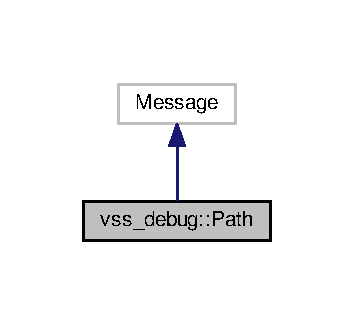
\includegraphics[width=170pt]{classvss__debug_1_1Path__inherit__graph}
\end{center}
\end{figure}


Diagrama de colaboração para vss\+\_\+debug\+:\+:Path\+:\nopagebreak
\begin{figure}[H]
\begin{center}
\leavevmode
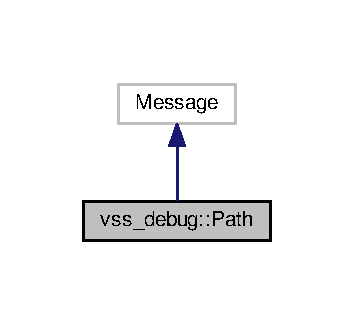
\includegraphics[width=170pt]{classvss__debug_1_1Path__coll__graph}
\end{center}
\end{figure}
\subsection*{Métodos Públicos}
\begin{DoxyCompactItemize}
\item 
{\bfseries Path} (const \hyperlink{classvss__debug_1_1Path}{Path} \&from)\hypertarget{classvss__debug_1_1Path_af4b9ca38ed432d20816a9827a72af76f}{}\label{classvss__debug_1_1Path_af4b9ca38ed432d20816a9827a72af76f}

\item 
\hyperlink{classvss__debug_1_1Path}{Path} \& {\bfseries operator=} (const \hyperlink{classvss__debug_1_1Path}{Path} \&from)\hypertarget{classvss__debug_1_1Path_a25616ef08c328c2f4fdcdc422cbcad19}{}\label{classvss__debug_1_1Path_a25616ef08c328c2f4fdcdc422cbcad19}

\item 
const \+::google\+::protobuf\+::\+Unknown\+Field\+Set \& {\bfseries unknown\+\_\+fields} () const \hypertarget{classvss__debug_1_1Path_a23c97dce09667e43b806194d70e6f6fa}{}\label{classvss__debug_1_1Path_a23c97dce09667e43b806194d70e6f6fa}

\item 
inline\+::google\+::protobuf\+::\+Unknown\+Field\+Set $\ast$ {\bfseries mutable\+\_\+unknown\+\_\+fields} ()\hypertarget{classvss__debug_1_1Path_ae7a2a47760d21cac3c3dc030660b1c06}{}\label{classvss__debug_1_1Path_ae7a2a47760d21cac3c3dc030660b1c06}

\item 
void {\bfseries Swap} (\hyperlink{classvss__debug_1_1Path}{Path} $\ast$other)\hypertarget{classvss__debug_1_1Path_aacc84278c4947fc416dcf1a494ef8082}{}\label{classvss__debug_1_1Path_aacc84278c4947fc416dcf1a494ef8082}

\item 
\hyperlink{classvss__debug_1_1Path}{Path} $\ast$ {\bfseries New} () const \hypertarget{classvss__debug_1_1Path_a2ac310685111c0e8cb05019d93763838}{}\label{classvss__debug_1_1Path_a2ac310685111c0e8cb05019d93763838}

\item 
\hyperlink{classvss__debug_1_1Path}{Path} $\ast$ {\bfseries New} (\+::google\+::protobuf\+::\+Arena $\ast$arena) const \hypertarget{classvss__debug_1_1Path_aa25fd596bb4efe2593f0fbbf3d06f49c}{}\label{classvss__debug_1_1Path_aa25fd596bb4efe2593f0fbbf3d06f49c}

\item 
void {\bfseries Copy\+From} (const \+::google\+::protobuf\+::\+Message \&from)\hypertarget{classvss__debug_1_1Path_a66bbe9b4220bba9d28470a33926e86e7}{}\label{classvss__debug_1_1Path_a66bbe9b4220bba9d28470a33926e86e7}

\item 
void {\bfseries Merge\+From} (const \+::google\+::protobuf\+::\+Message \&from)\hypertarget{classvss__debug_1_1Path_a9cd41c9f281451c410d4ed15fdef0f4f}{}\label{classvss__debug_1_1Path_a9cd41c9f281451c410d4ed15fdef0f4f}

\item 
void {\bfseries Copy\+From} (const \hyperlink{classvss__debug_1_1Path}{Path} \&from)\hypertarget{classvss__debug_1_1Path_ab030540eb875566f578b849d1e6446b1}{}\label{classvss__debug_1_1Path_ab030540eb875566f578b849d1e6446b1}

\item 
void {\bfseries Merge\+From} (const \hyperlink{classvss__debug_1_1Path}{Path} \&from)\hypertarget{classvss__debug_1_1Path_ae0d112d3a29dad98eedec19eb61cdb8e}{}\label{classvss__debug_1_1Path_ae0d112d3a29dad98eedec19eb61cdb8e}

\item 
void {\bfseries Clear} ()\hypertarget{classvss__debug_1_1Path_ac92857cedc93a91e0410aff6e9b9cb38}{}\label{classvss__debug_1_1Path_ac92857cedc93a91e0410aff6e9b9cb38}

\item 
bool {\bfseries Is\+Initialized} () const \hypertarget{classvss__debug_1_1Path_a3febb2d9f847dfacc28574552f656d43}{}\label{classvss__debug_1_1Path_a3febb2d9f847dfacc28574552f656d43}

\item 
int {\bfseries Byte\+Size} () const \hypertarget{classvss__debug_1_1Path_a70915c20ce71ac7597f1e9b4e4b0f580}{}\label{classvss__debug_1_1Path_a70915c20ce71ac7597f1e9b4e4b0f580}

\item 
bool {\bfseries Merge\+Partial\+From\+Coded\+Stream} (\+::google\+::protobuf\+::io\+::\+Coded\+Input\+Stream $\ast$input)\hypertarget{classvss__debug_1_1Path_a9b4f0f55454313f7a4a70d3a035f2451}{}\label{classvss__debug_1_1Path_a9b4f0f55454313f7a4a70d3a035f2451}

\item 
void {\bfseries Serialize\+With\+Cached\+Sizes} (\+::google\+::protobuf\+::io\+::\+Coded\+Output\+Stream $\ast$output) const \hypertarget{classvss__debug_1_1Path_a6286d44a76f30e0f324734b74b1ae99f}{}\label{classvss__debug_1_1Path_a6286d44a76f30e0f324734b74b1ae99f}

\item 
\+::google\+::protobuf\+::uint8 $\ast$ {\bfseries Internal\+Serialize\+With\+Cached\+Sizes\+To\+Array} (bool deterministic,\+::google\+::protobuf\+::uint8 $\ast$output) const \hypertarget{classvss__debug_1_1Path_a9d09fb5f3273d75d4f6735c47eecc159}{}\label{classvss__debug_1_1Path_a9d09fb5f3273d75d4f6735c47eecc159}

\item 
\+::google\+::protobuf\+::uint8 $\ast$ {\bfseries Serialize\+With\+Cached\+Sizes\+To\+Array} (\+::google\+::protobuf\+::uint8 $\ast$output) const \hypertarget{classvss__debug_1_1Path_ab6c9b95723a6dd2ff9442f1847168203}{}\label{classvss__debug_1_1Path_ab6c9b95723a6dd2ff9442f1847168203}

\item 
int {\bfseries Get\+Cached\+Size} () const \hypertarget{classvss__debug_1_1Path_a9a15a0e1a293dea45bcef786785753bd}{}\label{classvss__debug_1_1Path_a9a15a0e1a293dea45bcef786785753bd}

\item 
\+::google\+::protobuf\+::\+Metadata {\bfseries Get\+Metadata} () const \hypertarget{classvss__debug_1_1Path_a9aafbd0797871b8ea923044b6277a188}{}\label{classvss__debug_1_1Path_a9aafbd0797871b8ea923044b6277a188}

\item 
bool {\bfseries has\+\_\+id} () const \hypertarget{classvss__debug_1_1Path_a10b1ade3ecf8332cceb1762c863f3a84}{}\label{classvss__debug_1_1Path_a10b1ade3ecf8332cceb1762c863f3a84}

\item 
void {\bfseries clear\+\_\+id} ()\hypertarget{classvss__debug_1_1Path_a7f8c54f2e48f33e65b9802232231f534}{}\label{classvss__debug_1_1Path_a7f8c54f2e48f33e65b9802232231f534}

\item 
\+::google\+::protobuf\+::uint32 {\bfseries id} () const \hypertarget{classvss__debug_1_1Path_a561076a78a98f14815cd5245ea0b3d12}{}\label{classvss__debug_1_1Path_a561076a78a98f14815cd5245ea0b3d12}

\item 
void {\bfseries set\+\_\+id} (\+::google\+::protobuf\+::uint32 value)\hypertarget{classvss__debug_1_1Path_a96f82bb5726c2ec167d34c62fb1fa771}{}\label{classvss__debug_1_1Path_a96f82bb5726c2ec167d34c62fb1fa771}

\item 
int {\bfseries poses\+\_\+size} () const \hypertarget{classvss__debug_1_1Path_a265cd42a7398bea0f8fa78387315abd6}{}\label{classvss__debug_1_1Path_a265cd42a7398bea0f8fa78387315abd6}

\item 
void {\bfseries clear\+\_\+poses} ()\hypertarget{classvss__debug_1_1Path_add4628d195201c373f523238dba91b1c}{}\label{classvss__debug_1_1Path_add4628d195201c373f523238dba91b1c}

\item 
const \+::\hyperlink{classvss__debug_1_1Pose}{vss\+\_\+debug\+::\+Pose} \& {\bfseries poses} (int index) const \hypertarget{classvss__debug_1_1Path_a84192302b9ccefcba6fa7fc7b1073bd8}{}\label{classvss__debug_1_1Path_a84192302b9ccefcba6fa7fc7b1073bd8}

\item 
\+::\hyperlink{classvss__debug_1_1Pose}{vss\+\_\+debug\+::\+Pose} $\ast$ {\bfseries mutable\+\_\+poses} (int index)\hypertarget{classvss__debug_1_1Path_afcdcdbb2f516a6df6a871188ace9c415}{}\label{classvss__debug_1_1Path_afcdcdbb2f516a6df6a871188ace9c415}

\item 
\+::\hyperlink{classvss__debug_1_1Pose}{vss\+\_\+debug\+::\+Pose} $\ast$ {\bfseries add\+\_\+poses} ()\hypertarget{classvss__debug_1_1Path_aff82a92efa1b0968646598d6e2cb8a65}{}\label{classvss__debug_1_1Path_aff82a92efa1b0968646598d6e2cb8a65}

\item 
\+::google\+::protobuf\+::\+Repeated\+Ptr\+Field$<$ \+::\hyperlink{classvss__debug_1_1Pose}{vss\+\_\+debug\+::\+Pose} $>$ $\ast$ {\bfseries mutable\+\_\+poses} ()\hypertarget{classvss__debug_1_1Path_a2eb794be693f8207c6b3a08518effadd}{}\label{classvss__debug_1_1Path_a2eb794be693f8207c6b3a08518effadd}

\item 
const \+::google\+::protobuf\+::\+Repeated\+Ptr\+Field$<$ \+::\hyperlink{classvss__debug_1_1Pose}{vss\+\_\+debug\+::\+Pose} $>$ \& {\bfseries poses} () const \hypertarget{classvss__debug_1_1Path_a95c485b8485ddecfbdce3b3eaae88dd9}{}\label{classvss__debug_1_1Path_a95c485b8485ddecfbdce3b3eaae88dd9}

\end{DoxyCompactItemize}
\subsection*{Métodos Públicos Estáticos}
\begin{DoxyCompactItemize}
\item 
static const \+::google\+::protobuf\+::\+Descriptor $\ast$ {\bfseries descriptor} ()\hypertarget{classvss__debug_1_1Path_a8fcf1859c3c1c2250a4441a610f9abfb}{}\label{classvss__debug_1_1Path_a8fcf1859c3c1c2250a4441a610f9abfb}

\item 
static const \hyperlink{classvss__debug_1_1Path}{Path} \& {\bfseries default\+\_\+instance} ()\hypertarget{classvss__debug_1_1Path_a26996643d57311ecbe21fb145a9330fd}{}\label{classvss__debug_1_1Path_a26996643d57311ecbe21fb145a9330fd}

\end{DoxyCompactItemize}
\subsection*{Atributos Estáticos Públicos}
\begin{DoxyCompactItemize}
\item 
static const int {\bfseries k\+Id\+Field\+Number} = 1\hypertarget{classvss__debug_1_1Path_ab0c6d9a80fc2d5bac3bd83b3990b9f09}{}\label{classvss__debug_1_1Path_ab0c6d9a80fc2d5bac3bd83b3990b9f09}

\item 
static const int {\bfseries k\+Poses\+Field\+Number} = 2\hypertarget{classvss__debug_1_1Path_a4fc4f61c1caed01062dc10dfd2202380}{}\label{classvss__debug_1_1Path_a4fc4f61c1caed01062dc10dfd2202380}

\end{DoxyCompactItemize}
\subsection*{Amigas}
\begin{DoxyCompactItemize}
\item 
void {\bfseries protobuf\+\_\+\+Add\+Desc\+\_\+debug\+\_\+2eproto} ()\hypertarget{classvss__debug_1_1Path_a1b63d082883c064c19c50d8480e334a9}{}\label{classvss__debug_1_1Path_a1b63d082883c064c19c50d8480e334a9}

\item 
void {\bfseries protobuf\+\_\+\+Assign\+Desc\+\_\+debug\+\_\+2eproto} ()\hypertarget{classvss__debug_1_1Path_acdc8c7570bce883b7ac02f39e0d06b54}{}\label{classvss__debug_1_1Path_acdc8c7570bce883b7ac02f39e0d06b54}

\item 
void {\bfseries protobuf\+\_\+\+Shutdown\+File\+\_\+debug\+\_\+2eproto} ()\hypertarget{classvss__debug_1_1Path_a887dbf1466fd19ec2c6fb3c242c65a67}{}\label{classvss__debug_1_1Path_a887dbf1466fd19ec2c6fb3c242c65a67}

\end{DoxyCompactItemize}


A documentação para esta classe foi gerada a partir dos seguintes arquivos\+:\begin{DoxyCompactItemize}
\item 
/home/johnathan/\+Repositories/\+S\+I\+R\+Lab/\+Projects/\+V\+S\+S-\/\+Viewer/src/\+V\+S\+S-\/\+Interface/protos/debug.\+pb.\+h\item 
/home/johnathan/\+Repositories/\+S\+I\+R\+Lab/\+Projects/\+V\+S\+S-\/\+Viewer/src/\+V\+S\+S-\/\+Interface/protos/debug.\+pb.\+cc\end{DoxyCompactItemize}

\hypertarget{structcommon_1_1Pixel}{}\section{Referência da Estrutura common\+:\+:Pixel}
\label{structcommon_1_1Pixel}\index{common\+::\+Pixel@{common\+::\+Pixel}}


Essa struct é responsável por representar uma cor em R\+GB.  




{\ttfamily \#include $<$commons.\+h$>$}

\subsection*{Métodos Públicos}
\begin{DoxyCompactItemize}
\item 
\hyperlink{structcommon_1_1Pixel_ad8c36da59c20dd2b6f547e6dcbc7f273}{Pixel} ()\hypertarget{structcommon_1_1Pixel_ad8c36da59c20dd2b6f547e6dcbc7f273}{}\label{structcommon_1_1Pixel_ad8c36da59c20dd2b6f547e6dcbc7f273}

\begin{DoxyCompactList}\small\item\em Construtor D\+E\+F\+A\+U\+LT. \end{DoxyCompactList}\item 
\hyperlink{structcommon_1_1Pixel_aea7b41418980e0696fb78870d42abbe3}{Pixel} (float r, float g, float b)\hypertarget{structcommon_1_1Pixel_aea7b41418980e0696fb78870d42abbe3}{}\label{structcommon_1_1Pixel_aea7b41418980e0696fb78870d42abbe3}

\begin{DoxyCompactList}\small\item\em Construtor(r, g, b) \end{DoxyCompactList}\item 
\hyperlink{structcommon_1_1Pixel_a4a3df22498da4d45cbd0295e223470ed}{Pixel} (float \hyperlink{structcommon_1_1Pixel_abf3e7070359fa300aeed9af22c74f118}{rgb}\mbox{[}3\mbox{]})\hypertarget{structcommon_1_1Pixel_a4a3df22498da4d45cbd0295e223470ed}{}\label{structcommon_1_1Pixel_a4a3df22498da4d45cbd0295e223470ed}

\begin{DoxyCompactList}\small\item\em Construtor(rgb\mbox{[}3\mbox{]}) \end{DoxyCompactList}\item 
\hyperlink{structcommon_1_1Pixel_a7d987f23631f0695a2c8c8d5274842e0}{Pixel} (\hyperlink{structcommon_1_1Pixel}{Pixel} $\ast$p)\hypertarget{structcommon_1_1Pixel_a7d987f23631f0695a2c8c8d5274842e0}{}\label{structcommon_1_1Pixel_a7d987f23631f0695a2c8c8d5274842e0}

\begin{DoxyCompactList}\small\item\em Construtor cópia. \end{DoxyCompactList}\item 
void \hyperlink{structcommon_1_1Pixel_a384d642e3fb610b38c813ff6fd8c50e1}{show} ()\hypertarget{structcommon_1_1Pixel_a384d642e3fb610b38c813ff6fd8c50e1}{}\label{structcommon_1_1Pixel_a384d642e3fb610b38c813ff6fd8c50e1}

\begin{DoxyCompactList}\small\item\em Método de debug no terminal. \end{DoxyCompactList}\end{DoxyCompactItemize}
\subsection*{Atributos Públicos}
\begin{DoxyCompactItemize}
\item 
float \hyperlink{structcommon_1_1Pixel_abf3e7070359fa300aeed9af22c74f118}{rgb} \mbox{[}3\mbox{]}\hypertarget{structcommon_1_1Pixel_abf3e7070359fa300aeed9af22c74f118}{}\label{structcommon_1_1Pixel_abf3e7070359fa300aeed9af22c74f118}

\begin{DoxyCompactList}\small\item\em rgb\mbox{[}3\mbox{]}\+: rgb\mbox{[}r\mbox{]}, rgb\mbox{[}g\mbox{]}, rgb\mbox{[}b\mbox{]} \end{DoxyCompactList}\end{DoxyCompactItemize}


\subsection{Descrição Detalhada}
Essa struct é responsável por representar uma cor em R\+GB. 

A documentação para esta estrutura foi gerada a partir do seguinte arquivo\+:\begin{DoxyCompactItemize}
\item 
/home/johnathan/\+Repositories/\+S\+I\+R\+Lab/\+Public/\+V\+S\+S-\/\+Viewer/src/commons.\+h\end{DoxyCompactItemize}

\hypertarget{classvss__debug_1_1Pose}{}\section{Referência da Classe vss\+\_\+debug\+:\+:Pose}
\label{classvss__debug_1_1Pose}\index{vss\+\_\+debug\+::\+Pose@{vss\+\_\+debug\+::\+Pose}}


Diagrama de Hierarquia para vss\+\_\+debug\+:\+:Pose\+:\nopagebreak
\begin{figure}[H]
\begin{center}
\leavevmode
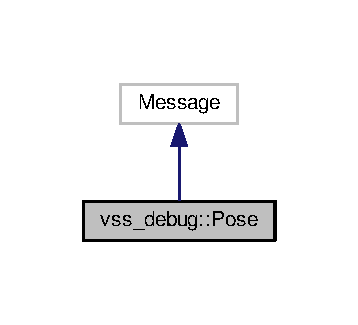
\includegraphics[width=172pt]{classvss__debug_1_1Pose__inherit__graph}
\end{center}
\end{figure}


Diagrama de colaboração para vss\+\_\+debug\+:\+:Pose\+:\nopagebreak
\begin{figure}[H]
\begin{center}
\leavevmode
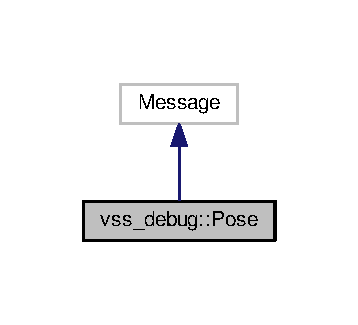
\includegraphics[width=172pt]{classvss__debug_1_1Pose__coll__graph}
\end{center}
\end{figure}
\subsection*{Métodos Públicos}
\begin{DoxyCompactItemize}
\item 
{\bfseries Pose} (const \hyperlink{classvss__debug_1_1Pose}{Pose} \&from)\hypertarget{classvss__debug_1_1Pose_ad24b46d4d64c036647334e838b1c56e8}{}\label{classvss__debug_1_1Pose_ad24b46d4d64c036647334e838b1c56e8}

\item 
\hyperlink{classvss__debug_1_1Pose}{Pose} \& {\bfseries operator=} (const \hyperlink{classvss__debug_1_1Pose}{Pose} \&from)\hypertarget{classvss__debug_1_1Pose_a34a3f9af832f1fe676b5daf2b9ac7b65}{}\label{classvss__debug_1_1Pose_a34a3f9af832f1fe676b5daf2b9ac7b65}

\item 
const \+::google\+::protobuf\+::\+Unknown\+Field\+Set \& {\bfseries unknown\+\_\+fields} () const \hypertarget{classvss__debug_1_1Pose_a58e4b7aaa136d3f70d2aab34d494d02e}{}\label{classvss__debug_1_1Pose_a58e4b7aaa136d3f70d2aab34d494d02e}

\item 
inline\+::google\+::protobuf\+::\+Unknown\+Field\+Set $\ast$ {\bfseries mutable\+\_\+unknown\+\_\+fields} ()\hypertarget{classvss__debug_1_1Pose_a2bc1876c70aec8f9a7c9cb9fd02d78ef}{}\label{classvss__debug_1_1Pose_a2bc1876c70aec8f9a7c9cb9fd02d78ef}

\item 
void {\bfseries Swap} (\hyperlink{classvss__debug_1_1Pose}{Pose} $\ast$other)\hypertarget{classvss__debug_1_1Pose_a3503ca66641a7d0311a0247a4561e3b1}{}\label{classvss__debug_1_1Pose_a3503ca66641a7d0311a0247a4561e3b1}

\item 
\hyperlink{classvss__debug_1_1Pose}{Pose} $\ast$ {\bfseries New} () const \hypertarget{classvss__debug_1_1Pose_a40be70547898f1a9f273a986b5a6ac05}{}\label{classvss__debug_1_1Pose_a40be70547898f1a9f273a986b5a6ac05}

\item 
\hyperlink{classvss__debug_1_1Pose}{Pose} $\ast$ {\bfseries New} (\+::google\+::protobuf\+::\+Arena $\ast$arena) const \hypertarget{classvss__debug_1_1Pose_a099d0a91b0491b81ac56b097daf6c8d8}{}\label{classvss__debug_1_1Pose_a099d0a91b0491b81ac56b097daf6c8d8}

\item 
void {\bfseries Copy\+From} (const \+::google\+::protobuf\+::\+Message \&from)\hypertarget{classvss__debug_1_1Pose_aa4ad68885b9773c051be4968da48a8ea}{}\label{classvss__debug_1_1Pose_aa4ad68885b9773c051be4968da48a8ea}

\item 
void {\bfseries Merge\+From} (const \+::google\+::protobuf\+::\+Message \&from)\hypertarget{classvss__debug_1_1Pose_a9c52bad876948ec4182d2c246f6e2a0d}{}\label{classvss__debug_1_1Pose_a9c52bad876948ec4182d2c246f6e2a0d}

\item 
void {\bfseries Copy\+From} (const \hyperlink{classvss__debug_1_1Pose}{Pose} \&from)\hypertarget{classvss__debug_1_1Pose_a4125d0ee96483793a5c8bbdacdfdce8a}{}\label{classvss__debug_1_1Pose_a4125d0ee96483793a5c8bbdacdfdce8a}

\item 
void {\bfseries Merge\+From} (const \hyperlink{classvss__debug_1_1Pose}{Pose} \&from)\hypertarget{classvss__debug_1_1Pose_a5a597ecd1ddff2e2ee5b84104960e2fa}{}\label{classvss__debug_1_1Pose_a5a597ecd1ddff2e2ee5b84104960e2fa}

\item 
void {\bfseries Clear} ()\hypertarget{classvss__debug_1_1Pose_a8f26357da9330adecfb3f238874b38c9}{}\label{classvss__debug_1_1Pose_a8f26357da9330adecfb3f238874b38c9}

\item 
bool {\bfseries Is\+Initialized} () const \hypertarget{classvss__debug_1_1Pose_a2f4c8f757103bb3a3de2b49a563f2ef4}{}\label{classvss__debug_1_1Pose_a2f4c8f757103bb3a3de2b49a563f2ef4}

\item 
int {\bfseries Byte\+Size} () const \hypertarget{classvss__debug_1_1Pose_af0f58169c73aba135cc58bd2361ca1e5}{}\label{classvss__debug_1_1Pose_af0f58169c73aba135cc58bd2361ca1e5}

\item 
bool {\bfseries Merge\+Partial\+From\+Coded\+Stream} (\+::google\+::protobuf\+::io\+::\+Coded\+Input\+Stream $\ast$input)\hypertarget{classvss__debug_1_1Pose_abc6b6c968cfc9995bb41c81f3902c888}{}\label{classvss__debug_1_1Pose_abc6b6c968cfc9995bb41c81f3902c888}

\item 
void {\bfseries Serialize\+With\+Cached\+Sizes} (\+::google\+::protobuf\+::io\+::\+Coded\+Output\+Stream $\ast$output) const \hypertarget{classvss__debug_1_1Pose_abb7022905e578e39930138239e7c11e4}{}\label{classvss__debug_1_1Pose_abb7022905e578e39930138239e7c11e4}

\item 
\+::google\+::protobuf\+::uint8 $\ast$ {\bfseries Internal\+Serialize\+With\+Cached\+Sizes\+To\+Array} (bool deterministic,\+::google\+::protobuf\+::uint8 $\ast$output) const \hypertarget{classvss__debug_1_1Pose_a762a458f4ab5d6cfa495ed5ec8b82790}{}\label{classvss__debug_1_1Pose_a762a458f4ab5d6cfa495ed5ec8b82790}

\item 
\+::google\+::protobuf\+::uint8 $\ast$ {\bfseries Serialize\+With\+Cached\+Sizes\+To\+Array} (\+::google\+::protobuf\+::uint8 $\ast$output) const \hypertarget{classvss__debug_1_1Pose_a9e10aa3d673a4f63862c2f66b80638c1}{}\label{classvss__debug_1_1Pose_a9e10aa3d673a4f63862c2f66b80638c1}

\item 
int {\bfseries Get\+Cached\+Size} () const \hypertarget{classvss__debug_1_1Pose_a46c892f974e6ba28a29ea32e27367c88}{}\label{classvss__debug_1_1Pose_a46c892f974e6ba28a29ea32e27367c88}

\item 
\+::google\+::protobuf\+::\+Metadata {\bfseries Get\+Metadata} () const \hypertarget{classvss__debug_1_1Pose_a98b13a5bc79f0d02a65a7ec85cb57789}{}\label{classvss__debug_1_1Pose_a98b13a5bc79f0d02a65a7ec85cb57789}

\item 
bool {\bfseries has\+\_\+id} () const \hypertarget{classvss__debug_1_1Pose_ad72613607a13a12b132e57c0fd756a25}{}\label{classvss__debug_1_1Pose_ad72613607a13a12b132e57c0fd756a25}

\item 
void {\bfseries clear\+\_\+id} ()\hypertarget{classvss__debug_1_1Pose_a327c72e990af33588f022f6bce4a5468}{}\label{classvss__debug_1_1Pose_a327c72e990af33588f022f6bce4a5468}

\item 
\+::google\+::protobuf\+::uint32 {\bfseries id} () const \hypertarget{classvss__debug_1_1Pose_aed2bcdb9df579a04e1a68dc2901d3584}{}\label{classvss__debug_1_1Pose_aed2bcdb9df579a04e1a68dc2901d3584}

\item 
void {\bfseries set\+\_\+id} (\+::google\+::protobuf\+::uint32 value)\hypertarget{classvss__debug_1_1Pose_abbf89801fee07e75b45b99414db5acf2}{}\label{classvss__debug_1_1Pose_abbf89801fee07e75b45b99414db5acf2}

\item 
bool {\bfseries has\+\_\+x} () const \hypertarget{classvss__debug_1_1Pose_a7dedd1bb04803183b4706163279f1115}{}\label{classvss__debug_1_1Pose_a7dedd1bb04803183b4706163279f1115}

\item 
void {\bfseries clear\+\_\+x} ()\hypertarget{classvss__debug_1_1Pose_a29bc420263638de043482d7a8ac58b9f}{}\label{classvss__debug_1_1Pose_a29bc420263638de043482d7a8ac58b9f}

\item 
float {\bfseries x} () const \hypertarget{classvss__debug_1_1Pose_a9dd4c62ce4845393ac1524b730aafad3}{}\label{classvss__debug_1_1Pose_a9dd4c62ce4845393ac1524b730aafad3}

\item 
void {\bfseries set\+\_\+x} (float value)\hypertarget{classvss__debug_1_1Pose_aa91cbb2787f184a7568c90c9ba685649}{}\label{classvss__debug_1_1Pose_aa91cbb2787f184a7568c90c9ba685649}

\item 
bool {\bfseries has\+\_\+y} () const \hypertarget{classvss__debug_1_1Pose_a352d2ea85d651ddee28e4d5eb74e56b3}{}\label{classvss__debug_1_1Pose_a352d2ea85d651ddee28e4d5eb74e56b3}

\item 
void {\bfseries clear\+\_\+y} ()\hypertarget{classvss__debug_1_1Pose_a5ef7077016c2ce7482e0330663e8c167}{}\label{classvss__debug_1_1Pose_a5ef7077016c2ce7482e0330663e8c167}

\item 
float {\bfseries y} () const \hypertarget{classvss__debug_1_1Pose_a7553d79057092bcbb1fc506ea146f068}{}\label{classvss__debug_1_1Pose_a7553d79057092bcbb1fc506ea146f068}

\item 
void {\bfseries set\+\_\+y} (float value)\hypertarget{classvss__debug_1_1Pose_a7ae6d05d4076bd94c413fb01025cc718}{}\label{classvss__debug_1_1Pose_a7ae6d05d4076bd94c413fb01025cc718}

\item 
bool {\bfseries has\+\_\+yaw} () const \hypertarget{classvss__debug_1_1Pose_ac8d4fa9306b4e96c1b6e12cdf14615ab}{}\label{classvss__debug_1_1Pose_ac8d4fa9306b4e96c1b6e12cdf14615ab}

\item 
void {\bfseries clear\+\_\+yaw} ()\hypertarget{classvss__debug_1_1Pose_a03023f32c8b5b03f2b75e7e642bab534}{}\label{classvss__debug_1_1Pose_a03023f32c8b5b03f2b75e7e642bab534}

\item 
float {\bfseries yaw} () const \hypertarget{classvss__debug_1_1Pose_ae6eb3a59a4788258597abdefef7b671b}{}\label{classvss__debug_1_1Pose_ae6eb3a59a4788258597abdefef7b671b}

\item 
void {\bfseries set\+\_\+yaw} (float value)\hypertarget{classvss__debug_1_1Pose_adfe61b426c995c1a95eba5d9b1d21fd4}{}\label{classvss__debug_1_1Pose_adfe61b426c995c1a95eba5d9b1d21fd4}

\end{DoxyCompactItemize}
\subsection*{Métodos Públicos Estáticos}
\begin{DoxyCompactItemize}
\item 
static const \+::google\+::protobuf\+::\+Descriptor $\ast$ {\bfseries descriptor} ()\hypertarget{classvss__debug_1_1Pose_a3d781b52c5eb085b6c826f82c216f373}{}\label{classvss__debug_1_1Pose_a3d781b52c5eb085b6c826f82c216f373}

\item 
static const \hyperlink{classvss__debug_1_1Pose}{Pose} \& {\bfseries default\+\_\+instance} ()\hypertarget{classvss__debug_1_1Pose_ae87e9b283f3406bafcb9412dc889f5f6}{}\label{classvss__debug_1_1Pose_ae87e9b283f3406bafcb9412dc889f5f6}

\end{DoxyCompactItemize}
\subsection*{Atributos Estáticos Públicos}
\begin{DoxyCompactItemize}
\item 
static const int {\bfseries k\+Id\+Field\+Number} = 1\hypertarget{classvss__debug_1_1Pose_ac1628279f5a8d48ca973175edd43620a}{}\label{classvss__debug_1_1Pose_ac1628279f5a8d48ca973175edd43620a}

\item 
static const int {\bfseries k\+X\+Field\+Number} = 2\hypertarget{classvss__debug_1_1Pose_a6abea7e231aa91207b15d554976fb877}{}\label{classvss__debug_1_1Pose_a6abea7e231aa91207b15d554976fb877}

\item 
static const int {\bfseries k\+Y\+Field\+Number} = 3\hypertarget{classvss__debug_1_1Pose_a9330e946308fc1a78c01fcc9563ac017}{}\label{classvss__debug_1_1Pose_a9330e946308fc1a78c01fcc9563ac017}

\item 
static const int {\bfseries k\+Yaw\+Field\+Number} = 4\hypertarget{classvss__debug_1_1Pose_a23e9fa2a03ccd5d99a6aa14c0e801346}{}\label{classvss__debug_1_1Pose_a23e9fa2a03ccd5d99a6aa14c0e801346}

\end{DoxyCompactItemize}
\subsection*{Amigas}
\begin{DoxyCompactItemize}
\item 
void {\bfseries protobuf\+\_\+\+Add\+Desc\+\_\+debug\+\_\+2eproto} ()\hypertarget{classvss__debug_1_1Pose_a1b63d082883c064c19c50d8480e334a9}{}\label{classvss__debug_1_1Pose_a1b63d082883c064c19c50d8480e334a9}

\item 
void {\bfseries protobuf\+\_\+\+Assign\+Desc\+\_\+debug\+\_\+2eproto} ()\hypertarget{classvss__debug_1_1Pose_acdc8c7570bce883b7ac02f39e0d06b54}{}\label{classvss__debug_1_1Pose_acdc8c7570bce883b7ac02f39e0d06b54}

\item 
void {\bfseries protobuf\+\_\+\+Shutdown\+File\+\_\+debug\+\_\+2eproto} ()\hypertarget{classvss__debug_1_1Pose_a887dbf1466fd19ec2c6fb3c242c65a67}{}\label{classvss__debug_1_1Pose_a887dbf1466fd19ec2c6fb3c242c65a67}

\end{DoxyCompactItemize}


A documentação para esta classe foi gerada a partir dos seguintes arquivos\+:\begin{DoxyCompactItemize}
\item 
/home/johnathan/\+Repositories/\+S\+I\+R\+Lab/\+Public/\+V\+S\+S-\/\+Viewer/src/\+V\+S\+S-\/\+Interface/protos/debug.\+pb.\+h\item 
/home/johnathan/\+Repositories/\+S\+I\+R\+Lab/\+Public/\+V\+S\+S-\/\+Viewer/src/\+V\+S\+S-\/\+Interface/protos/debug.\+pb.\+cc\end{DoxyCompactItemize}

\hypertarget{classvss__state_1_1Pose}{}\section{Referência da Classe vss\+\_\+state\+:\+:Pose}
\label{classvss__state_1_1Pose}\index{vss\+\_\+state\+::\+Pose@{vss\+\_\+state\+::\+Pose}}


Diagrama de Hierarquia para vss\+\_\+state\+:\+:Pose\+:\nopagebreak
\begin{figure}[H]
\begin{center}
\leavevmode
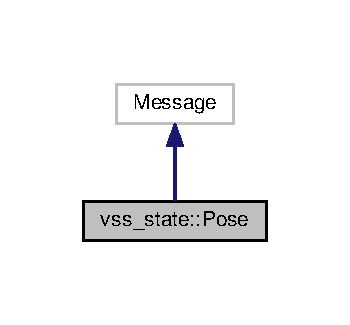
\includegraphics[width=168pt]{classvss__state_1_1Pose__inherit__graph}
\end{center}
\end{figure}


Diagrama de colaboração para vss\+\_\+state\+:\+:Pose\+:\nopagebreak
\begin{figure}[H]
\begin{center}
\leavevmode
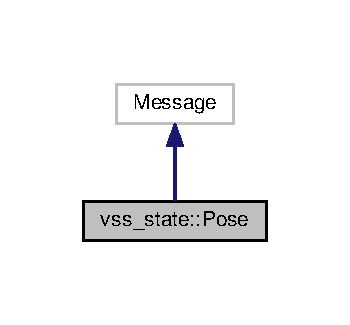
\includegraphics[width=168pt]{classvss__state_1_1Pose__coll__graph}
\end{center}
\end{figure}
\subsection*{Métodos Públicos}
\begin{DoxyCompactItemize}
\item 
{\bfseries Pose} (const \hyperlink{classvss__state_1_1Pose}{Pose} \&from)\hypertarget{classvss__state_1_1Pose_afbd08781a545cc0d5b06623f929e80c7}{}\label{classvss__state_1_1Pose_afbd08781a545cc0d5b06623f929e80c7}

\item 
\hyperlink{classvss__state_1_1Pose}{Pose} \& {\bfseries operator=} (const \hyperlink{classvss__state_1_1Pose}{Pose} \&from)\hypertarget{classvss__state_1_1Pose_af5acd047e2b69e6fbb54592bbf599bfc}{}\label{classvss__state_1_1Pose_af5acd047e2b69e6fbb54592bbf599bfc}

\item 
const \+::google\+::protobuf\+::\+Unknown\+Field\+Set \& {\bfseries unknown\+\_\+fields} () const \hypertarget{classvss__state_1_1Pose_a6c3b4c8e189c186061297043d00b68bb}{}\label{classvss__state_1_1Pose_a6c3b4c8e189c186061297043d00b68bb}

\item 
inline\+::google\+::protobuf\+::\+Unknown\+Field\+Set $\ast$ {\bfseries mutable\+\_\+unknown\+\_\+fields} ()\hypertarget{classvss__state_1_1Pose_a76aee4c2024d80ffe335e65907434dee}{}\label{classvss__state_1_1Pose_a76aee4c2024d80ffe335e65907434dee}

\item 
void {\bfseries Swap} (\hyperlink{classvss__state_1_1Pose}{Pose} $\ast$other)\hypertarget{classvss__state_1_1Pose_a6288b4add8dde23e78f2dd0a54ddc00a}{}\label{classvss__state_1_1Pose_a6288b4add8dde23e78f2dd0a54ddc00a}

\item 
\hyperlink{classvss__state_1_1Pose}{Pose} $\ast$ {\bfseries New} () const \hypertarget{classvss__state_1_1Pose_ac5df28dce77b8c3566505950585528c3}{}\label{classvss__state_1_1Pose_ac5df28dce77b8c3566505950585528c3}

\item 
\hyperlink{classvss__state_1_1Pose}{Pose} $\ast$ {\bfseries New} (\+::google\+::protobuf\+::\+Arena $\ast$arena) const \hypertarget{classvss__state_1_1Pose_aa47e4b4bbbce2532645868c51c4ee96b}{}\label{classvss__state_1_1Pose_aa47e4b4bbbce2532645868c51c4ee96b}

\item 
void {\bfseries Copy\+From} (const \+::google\+::protobuf\+::\+Message \&from)\hypertarget{classvss__state_1_1Pose_a6e17322c8f9d53e131ed8e1702aefcd3}{}\label{classvss__state_1_1Pose_a6e17322c8f9d53e131ed8e1702aefcd3}

\item 
void {\bfseries Merge\+From} (const \+::google\+::protobuf\+::\+Message \&from)\hypertarget{classvss__state_1_1Pose_aa1e7e92d17b26dce271b698e86145d2b}{}\label{classvss__state_1_1Pose_aa1e7e92d17b26dce271b698e86145d2b}

\item 
void {\bfseries Copy\+From} (const \hyperlink{classvss__state_1_1Pose}{Pose} \&from)\hypertarget{classvss__state_1_1Pose_a29467f35bd2186cb7e781eea648a8c3b}{}\label{classvss__state_1_1Pose_a29467f35bd2186cb7e781eea648a8c3b}

\item 
void {\bfseries Merge\+From} (const \hyperlink{classvss__state_1_1Pose}{Pose} \&from)\hypertarget{classvss__state_1_1Pose_a679b672f248c7a53c203465eb3dca328}{}\label{classvss__state_1_1Pose_a679b672f248c7a53c203465eb3dca328}

\item 
void {\bfseries Clear} ()\hypertarget{classvss__state_1_1Pose_a57b811afbc5889b23ad1713684619132}{}\label{classvss__state_1_1Pose_a57b811afbc5889b23ad1713684619132}

\item 
bool {\bfseries Is\+Initialized} () const \hypertarget{classvss__state_1_1Pose_a06a7663fb631cbc15bbdccb88d42d835}{}\label{classvss__state_1_1Pose_a06a7663fb631cbc15bbdccb88d42d835}

\item 
int {\bfseries Byte\+Size} () const \hypertarget{classvss__state_1_1Pose_a96e59891029ae382fd88854eea96b223}{}\label{classvss__state_1_1Pose_a96e59891029ae382fd88854eea96b223}

\item 
bool {\bfseries Merge\+Partial\+From\+Coded\+Stream} (\+::google\+::protobuf\+::io\+::\+Coded\+Input\+Stream $\ast$input)\hypertarget{classvss__state_1_1Pose_aad871e3c8d77d794b785e512d60e440c}{}\label{classvss__state_1_1Pose_aad871e3c8d77d794b785e512d60e440c}

\item 
void {\bfseries Serialize\+With\+Cached\+Sizes} (\+::google\+::protobuf\+::io\+::\+Coded\+Output\+Stream $\ast$output) const \hypertarget{classvss__state_1_1Pose_af1e240831f2cb26edfc3d2f9bc4583d4}{}\label{classvss__state_1_1Pose_af1e240831f2cb26edfc3d2f9bc4583d4}

\item 
\+::google\+::protobuf\+::uint8 $\ast$ {\bfseries Internal\+Serialize\+With\+Cached\+Sizes\+To\+Array} (bool deterministic,\+::google\+::protobuf\+::uint8 $\ast$output) const \hypertarget{classvss__state_1_1Pose_acc3af009b98896daefdfd7d78166b1ed}{}\label{classvss__state_1_1Pose_acc3af009b98896daefdfd7d78166b1ed}

\item 
\+::google\+::protobuf\+::uint8 $\ast$ {\bfseries Serialize\+With\+Cached\+Sizes\+To\+Array} (\+::google\+::protobuf\+::uint8 $\ast$output) const \hypertarget{classvss__state_1_1Pose_a468f58ed7eacafe41fd9ae4c57b9e455}{}\label{classvss__state_1_1Pose_a468f58ed7eacafe41fd9ae4c57b9e455}

\item 
int {\bfseries Get\+Cached\+Size} () const \hypertarget{classvss__state_1_1Pose_a97a32d12afefa90b01e0b6ed6713bb18}{}\label{classvss__state_1_1Pose_a97a32d12afefa90b01e0b6ed6713bb18}

\item 
\+::google\+::protobuf\+::\+Metadata {\bfseries Get\+Metadata} () const \hypertarget{classvss__state_1_1Pose_a318666ae85650504a7dd7f2418b01e0c}{}\label{classvss__state_1_1Pose_a318666ae85650504a7dd7f2418b01e0c}

\item 
bool {\bfseries has\+\_\+x} () const \hypertarget{classvss__state_1_1Pose_a60f0b9173d18d8845c77d24e6d76332a}{}\label{classvss__state_1_1Pose_a60f0b9173d18d8845c77d24e6d76332a}

\item 
void {\bfseries clear\+\_\+x} ()\hypertarget{classvss__state_1_1Pose_a4d62819148aa3020a288e9868a0006f3}{}\label{classvss__state_1_1Pose_a4d62819148aa3020a288e9868a0006f3}

\item 
float {\bfseries x} () const \hypertarget{classvss__state_1_1Pose_ab391726391e1e7b9f87e06b7edcc1768}{}\label{classvss__state_1_1Pose_ab391726391e1e7b9f87e06b7edcc1768}

\item 
void {\bfseries set\+\_\+x} (float value)\hypertarget{classvss__state_1_1Pose_aed73f2b005cdb676836600da66a7b8ce}{}\label{classvss__state_1_1Pose_aed73f2b005cdb676836600da66a7b8ce}

\item 
bool {\bfseries has\+\_\+y} () const \hypertarget{classvss__state_1_1Pose_abee5671e3f6cc80e5c71eb157e852f1b}{}\label{classvss__state_1_1Pose_abee5671e3f6cc80e5c71eb157e852f1b}

\item 
void {\bfseries clear\+\_\+y} ()\hypertarget{classvss__state_1_1Pose_adf20a0255b343918c583c1b990422190}{}\label{classvss__state_1_1Pose_adf20a0255b343918c583c1b990422190}

\item 
float {\bfseries y} () const \hypertarget{classvss__state_1_1Pose_a413b079a4e1261a1694c148f7bd8cc76}{}\label{classvss__state_1_1Pose_a413b079a4e1261a1694c148f7bd8cc76}

\item 
void {\bfseries set\+\_\+y} (float value)\hypertarget{classvss__state_1_1Pose_a8f9ff5d89e9ce9cd1de1f3a707efc65f}{}\label{classvss__state_1_1Pose_a8f9ff5d89e9ce9cd1de1f3a707efc65f}

\item 
bool {\bfseries has\+\_\+yaw} () const \hypertarget{classvss__state_1_1Pose_ae9e89cd7eee237cfd7333449e3381cad}{}\label{classvss__state_1_1Pose_ae9e89cd7eee237cfd7333449e3381cad}

\item 
void {\bfseries clear\+\_\+yaw} ()\hypertarget{classvss__state_1_1Pose_adaf3f1567e367b89722e45b4bcc8bff6}{}\label{classvss__state_1_1Pose_adaf3f1567e367b89722e45b4bcc8bff6}

\item 
float {\bfseries yaw} () const \hypertarget{classvss__state_1_1Pose_a0b8e24e17a194af015f54ee616f583ab}{}\label{classvss__state_1_1Pose_a0b8e24e17a194af015f54ee616f583ab}

\item 
void {\bfseries set\+\_\+yaw} (float value)\hypertarget{classvss__state_1_1Pose_a7ec9dc6ed0302298048cd803e96b6ca3}{}\label{classvss__state_1_1Pose_a7ec9dc6ed0302298048cd803e96b6ca3}

\end{DoxyCompactItemize}
\subsection*{Métodos Públicos Estáticos}
\begin{DoxyCompactItemize}
\item 
static const \+::google\+::protobuf\+::\+Descriptor $\ast$ {\bfseries descriptor} ()\hypertarget{classvss__state_1_1Pose_a6423cf6dd9db285c52d1bb4e10e1a24c}{}\label{classvss__state_1_1Pose_a6423cf6dd9db285c52d1bb4e10e1a24c}

\item 
static const \hyperlink{classvss__state_1_1Pose}{Pose} \& {\bfseries default\+\_\+instance} ()\hypertarget{classvss__state_1_1Pose_a6d403e8d406ba3fd0403662cf8883fcc}{}\label{classvss__state_1_1Pose_a6d403e8d406ba3fd0403662cf8883fcc}

\end{DoxyCompactItemize}
\subsection*{Atributos Estáticos Públicos}
\begin{DoxyCompactItemize}
\item 
static const int {\bfseries k\+X\+Field\+Number} = 1\hypertarget{classvss__state_1_1Pose_a55da0ea3762949322b44da8206bb84f0}{}\label{classvss__state_1_1Pose_a55da0ea3762949322b44da8206bb84f0}

\item 
static const int {\bfseries k\+Y\+Field\+Number} = 2\hypertarget{classvss__state_1_1Pose_a0a2f401726b1453c65cbaa99fde61b4e}{}\label{classvss__state_1_1Pose_a0a2f401726b1453c65cbaa99fde61b4e}

\item 
static const int {\bfseries k\+Yaw\+Field\+Number} = 3\hypertarget{classvss__state_1_1Pose_a4f1b9b7cb0a470421a29a733329a7e7c}{}\label{classvss__state_1_1Pose_a4f1b9b7cb0a470421a29a733329a7e7c}

\end{DoxyCompactItemize}
\subsection*{Amigas}
\begin{DoxyCompactItemize}
\item 
void {\bfseries protobuf\+\_\+\+Add\+Desc\+\_\+state\+\_\+2eproto} ()\hypertarget{classvss__state_1_1Pose_aab1a2c258f8122a403a979ff57e2a706}{}\label{classvss__state_1_1Pose_aab1a2c258f8122a403a979ff57e2a706}

\item 
void {\bfseries protobuf\+\_\+\+Assign\+Desc\+\_\+state\+\_\+2eproto} ()\hypertarget{classvss__state_1_1Pose_a57d9367bc8a7a94ead11d11194cca1b6}{}\label{classvss__state_1_1Pose_a57d9367bc8a7a94ead11d11194cca1b6}

\item 
void {\bfseries protobuf\+\_\+\+Shutdown\+File\+\_\+state\+\_\+2eproto} ()\hypertarget{classvss__state_1_1Pose_a4e6dc5e8e72799859c4e9556d090e57d}{}\label{classvss__state_1_1Pose_a4e6dc5e8e72799859c4e9556d090e57d}

\end{DoxyCompactItemize}


A documentação para esta classe foi gerada a partir dos seguintes arquivos\+:\begin{DoxyCompactItemize}
\item 
/home/johnathan/\+Repositories/\+S\+I\+R\+Lab/\+Public/\+V\+S\+S-\/\+Viewer/src/\+V\+S\+S-\/\+Interface/protos/state.\+pb.\+h\item 
/home/johnathan/\+Repositories/\+S\+I\+R\+Lab/\+Public/\+V\+S\+S-\/\+Viewer/src/\+V\+S\+S-\/\+Interface/protos/state.\+pb.\+cc\end{DoxyCompactItemize}

\hypertarget{structcommon_1_1Pose}{}\section{Referência da Estrutura common\+:\+:Pose}
\label{structcommon_1_1Pose}\index{common\+::\+Pose@{common\+::\+Pose}}


Essa struct é responsável por representar uma \hyperlink{structcommon_1_1Pose}{Pose}, isto é, Posição e Orientação de um corpo rígido do espaço do futebol de robôs.  




{\ttfamily \#include $<$commons.\+h$>$}

\subsection*{Métodos Públicos}
\begin{DoxyCompactItemize}
\item 
\hyperlink{structcommon_1_1Pose_ae8d335bc9fd48b9a28f75b29c0d87581}{Pose} ()\hypertarget{structcommon_1_1Pose_ae8d335bc9fd48b9a28f75b29c0d87581}{}\label{structcommon_1_1Pose_ae8d335bc9fd48b9a28f75b29c0d87581}

\begin{DoxyCompactList}\small\item\em Construtor D\+E\+F\+A\+U\+LT. \end{DoxyCompactList}\item 
\hyperlink{structcommon_1_1Pose_a13c5329282b42ce481d6c161117c708d}{Pose} (float \hyperlink{structcommon_1_1Pose_a4ea360bde6890187e0a8ce0ca57fa031}{x}, float \hyperlink{structcommon_1_1Pose_aa7debd220c3cb6f294253188045a4d0d}{y}, float \hyperlink{structcommon_1_1Pose_a6abb6006c34912516585beeb33077c6c}{yaw})\hypertarget{structcommon_1_1Pose_a13c5329282b42ce481d6c161117c708d}{}\label{structcommon_1_1Pose_a13c5329282b42ce481d6c161117c708d}

\begin{DoxyCompactList}\small\item\em Construtor(x, y, yaw) \end{DoxyCompactList}\item 
\hyperlink{structcommon_1_1Pose_a54bb645f2fa8043de902b6cfa0b7c90e}{Pose} (\hyperlink{structcommon_1_1Pose}{Pose} $\ast$p)\hypertarget{structcommon_1_1Pose_a54bb645f2fa8043de902b6cfa0b7c90e}{}\label{structcommon_1_1Pose_a54bb645f2fa8043de902b6cfa0b7c90e}

\begin{DoxyCompactList}\small\item\em Construtor cópia. \end{DoxyCompactList}\item 
void \hyperlink{structcommon_1_1Pose_a41bd06a4fc95fc1cdac527fab6ef4d21}{show} ()\hypertarget{structcommon_1_1Pose_a41bd06a4fc95fc1cdac527fab6ef4d21}{}\label{structcommon_1_1Pose_a41bd06a4fc95fc1cdac527fab6ef4d21}

\begin{DoxyCompactList}\small\item\em Método de debug no terminal. \end{DoxyCompactList}\end{DoxyCompactItemize}
\subsection*{Atributos Públicos}
\begin{DoxyCompactItemize}
\item 
float \hyperlink{structcommon_1_1Pose_a4ea360bde6890187e0a8ce0ca57fa031}{x}\hypertarget{structcommon_1_1Pose_a4ea360bde6890187e0a8ce0ca57fa031}{}\label{structcommon_1_1Pose_a4ea360bde6890187e0a8ce0ca57fa031}

\begin{DoxyCompactList}\small\item\em Posição em X. \end{DoxyCompactList}\item 
float \hyperlink{structcommon_1_1Pose_aa7debd220c3cb6f294253188045a4d0d}{y}\hypertarget{structcommon_1_1Pose_aa7debd220c3cb6f294253188045a4d0d}{}\label{structcommon_1_1Pose_aa7debd220c3cb6f294253188045a4d0d}

\begin{DoxyCompactList}\small\item\em Posição em Y. \end{DoxyCompactList}\item 
float \hyperlink{structcommon_1_1Pose_a6abb6006c34912516585beeb33077c6c}{yaw}\hypertarget{structcommon_1_1Pose_a6abb6006c34912516585beeb33077c6c}{}\label{structcommon_1_1Pose_a6abb6006c34912516585beeb33077c6c}

\begin{DoxyCompactList}\small\item\em Orientação em Z. \end{DoxyCompactList}\end{DoxyCompactItemize}


\subsection{Descrição Detalhada}
Essa struct é responsável por representar uma \hyperlink{structcommon_1_1Pose}{Pose}, isto é, Posição e Orientação de um corpo rígido do espaço do futebol de robôs. 

A documentação para esta estrutura foi gerada a partir do seguinte arquivo\+:\begin{DoxyCompactItemize}
\item 
/home/johnathan/\+Repositories/\+S\+I\+R\+Lab/\+Public/\+V\+S\+S-\/\+Viewer/src/commons.\+h\end{DoxyCompactItemize}

\hypertarget{classvss__state_1_1RGB}{}\section{Referência da Classe vss\+\_\+state\+:\+:R\+GB}
\label{classvss__state_1_1RGB}\index{vss\+\_\+state\+::\+R\+GB@{vss\+\_\+state\+::\+R\+GB}}


Diagrama de Hierarquia para vss\+\_\+state\+:\+:R\+GB\+:\nopagebreak
\begin{figure}[H]
\begin{center}
\leavevmode
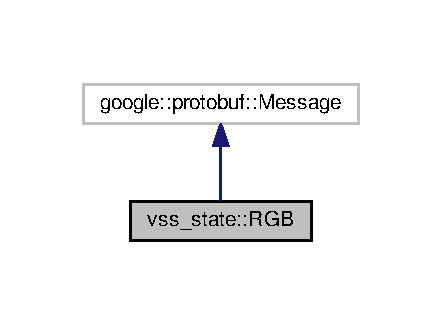
\includegraphics[width=212pt]{classvss__state_1_1RGB__inherit__graph}
\end{center}
\end{figure}


Diagrama de colaboração para vss\+\_\+state\+:\+:R\+GB\+:\nopagebreak
\begin{figure}[H]
\begin{center}
\leavevmode
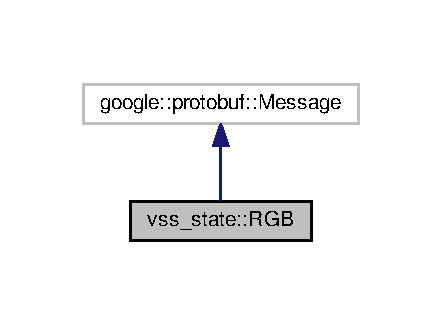
\includegraphics[width=212pt]{classvss__state_1_1RGB__coll__graph}
\end{center}
\end{figure}
\subsection*{Métodos Públicos}
\begin{DoxyCompactItemize}
\item 
{\bfseries R\+GB} (const \hyperlink{classvss__state_1_1RGB}{R\+GB} \&from)\hypertarget{classvss__state_1_1RGB_ad057f22713ee486fa88d59661f15c390}{}\label{classvss__state_1_1RGB_ad057f22713ee486fa88d59661f15c390}

\item 
\hyperlink{classvss__state_1_1RGB}{R\+GB} \& {\bfseries operator=} (const \hyperlink{classvss__state_1_1RGB}{R\+GB} \&from)\hypertarget{classvss__state_1_1RGB_ae6850f3550d012f10cb3fe961ceca13a}{}\label{classvss__state_1_1RGB_ae6850f3550d012f10cb3fe961ceca13a}

\item 
const \+::google\+::protobuf\+::\+Unknown\+Field\+Set \& {\bfseries unknown\+\_\+fields} () const \hypertarget{classvss__state_1_1RGB_af3633b5c052c9b983f03dca86c5172e3}{}\label{classvss__state_1_1RGB_af3633b5c052c9b983f03dca86c5172e3}

\item 
inline\+::google\+::protobuf\+::\+Unknown\+Field\+Set $\ast$ {\bfseries mutable\+\_\+unknown\+\_\+fields} ()\hypertarget{classvss__state_1_1RGB_adfdaca9126b92f913d030d86975fb390}{}\label{classvss__state_1_1RGB_adfdaca9126b92f913d030d86975fb390}

\item 
void {\bfseries Swap} (\hyperlink{classvss__state_1_1RGB}{R\+GB} $\ast$other)\hypertarget{classvss__state_1_1RGB_a42f05e54d0dc837400c5079899b463aa}{}\label{classvss__state_1_1RGB_a42f05e54d0dc837400c5079899b463aa}

\item 
\hyperlink{classvss__state_1_1RGB}{R\+GB} $\ast$ {\bfseries New} () const \hypertarget{classvss__state_1_1RGB_af84170737e8c4116c9a2f85dc11a3503}{}\label{classvss__state_1_1RGB_af84170737e8c4116c9a2f85dc11a3503}

\item 
\hyperlink{classvss__state_1_1RGB}{R\+GB} $\ast$ {\bfseries New} (\+::google\+::protobuf\+::\+Arena $\ast$arena) const \hypertarget{classvss__state_1_1RGB_a275fa538a9a801635e12e94d188acf82}{}\label{classvss__state_1_1RGB_a275fa538a9a801635e12e94d188acf82}

\item 
void {\bfseries Copy\+From} (const \+::google\+::protobuf\+::\+Message \&from)\hypertarget{classvss__state_1_1RGB_a7dca7dca78106990bae0191f4fc58aa3}{}\label{classvss__state_1_1RGB_a7dca7dca78106990bae0191f4fc58aa3}

\item 
void {\bfseries Merge\+From} (const \+::google\+::protobuf\+::\+Message \&from)\hypertarget{classvss__state_1_1RGB_a6b287c534b5414da22c85a7ace395032}{}\label{classvss__state_1_1RGB_a6b287c534b5414da22c85a7ace395032}

\item 
void {\bfseries Copy\+From} (const \hyperlink{classvss__state_1_1RGB}{R\+GB} \&from)\hypertarget{classvss__state_1_1RGB_af67ab2848e2357d23f411c0df8bce782}{}\label{classvss__state_1_1RGB_af67ab2848e2357d23f411c0df8bce782}

\item 
void {\bfseries Merge\+From} (const \hyperlink{classvss__state_1_1RGB}{R\+GB} \&from)\hypertarget{classvss__state_1_1RGB_a168e56eb490d40877481d8a709ae8322}{}\label{classvss__state_1_1RGB_a168e56eb490d40877481d8a709ae8322}

\item 
void {\bfseries Clear} ()\hypertarget{classvss__state_1_1RGB_ad0c9a1848a43f2d89ebaa33d51ac6634}{}\label{classvss__state_1_1RGB_ad0c9a1848a43f2d89ebaa33d51ac6634}

\item 
bool {\bfseries Is\+Initialized} () const \hypertarget{classvss__state_1_1RGB_a0d2e0b5f89279b7553ef83d702f0bab8}{}\label{classvss__state_1_1RGB_a0d2e0b5f89279b7553ef83d702f0bab8}

\item 
int {\bfseries Byte\+Size} () const \hypertarget{classvss__state_1_1RGB_a2cd250a169ec6f47428b72537d384bcd}{}\label{classvss__state_1_1RGB_a2cd250a169ec6f47428b72537d384bcd}

\item 
bool {\bfseries Merge\+Partial\+From\+Coded\+Stream} (\+::google\+::protobuf\+::io\+::\+Coded\+Input\+Stream $\ast$input)\hypertarget{classvss__state_1_1RGB_a2e6177a7e8c631c1f62a2d986fdfc452}{}\label{classvss__state_1_1RGB_a2e6177a7e8c631c1f62a2d986fdfc452}

\item 
void {\bfseries Serialize\+With\+Cached\+Sizes} (\+::google\+::protobuf\+::io\+::\+Coded\+Output\+Stream $\ast$output) const \hypertarget{classvss__state_1_1RGB_ab16a3fd0ce7788dd974d078e445e7849}{}\label{classvss__state_1_1RGB_ab16a3fd0ce7788dd974d078e445e7849}

\item 
\+::google\+::protobuf\+::uint8 $\ast$ {\bfseries Internal\+Serialize\+With\+Cached\+Sizes\+To\+Array} (bool deterministic,\+::google\+::protobuf\+::uint8 $\ast$output) const \hypertarget{classvss__state_1_1RGB_af94a48e2086eab7b6f8a3787e7277bcf}{}\label{classvss__state_1_1RGB_af94a48e2086eab7b6f8a3787e7277bcf}

\item 
\+::google\+::protobuf\+::uint8 $\ast$ {\bfseries Serialize\+With\+Cached\+Sizes\+To\+Array} (\+::google\+::protobuf\+::uint8 $\ast$output) const \hypertarget{classvss__state_1_1RGB_a5b53556c120673ad274fc0304bf33a0d}{}\label{classvss__state_1_1RGB_a5b53556c120673ad274fc0304bf33a0d}

\item 
int {\bfseries Get\+Cached\+Size} () const \hypertarget{classvss__state_1_1RGB_a40f2c075e63a05d37dd4023cd25c61e6}{}\label{classvss__state_1_1RGB_a40f2c075e63a05d37dd4023cd25c61e6}

\item 
\+::google\+::protobuf\+::\+Metadata {\bfseries Get\+Metadata} () const \hypertarget{classvss__state_1_1RGB_a72a71c6babca0d3cbd79caf9d8c9c9b2}{}\label{classvss__state_1_1RGB_a72a71c6babca0d3cbd79caf9d8c9c9b2}

\item 
bool {\bfseries has\+\_\+r} () const \hypertarget{classvss__state_1_1RGB_a44a2e2f01894715c2732c8455a27c158}{}\label{classvss__state_1_1RGB_a44a2e2f01894715c2732c8455a27c158}

\item 
void {\bfseries clear\+\_\+r} ()\hypertarget{classvss__state_1_1RGB_acf08083664a7f2da6c10b8faf4b25383}{}\label{classvss__state_1_1RGB_acf08083664a7f2da6c10b8faf4b25383}

\item 
\+::google\+::protobuf\+::uint32 {\bfseries r} () const \hypertarget{classvss__state_1_1RGB_ab1fb0a4d6eebeb673bc32c90b1b906ed}{}\label{classvss__state_1_1RGB_ab1fb0a4d6eebeb673bc32c90b1b906ed}

\item 
void {\bfseries set\+\_\+r} (\+::google\+::protobuf\+::uint32 value)\hypertarget{classvss__state_1_1RGB_a33dd755c711c8a7f5a1897e42ea4c711}{}\label{classvss__state_1_1RGB_a33dd755c711c8a7f5a1897e42ea4c711}

\item 
bool {\bfseries has\+\_\+g} () const \hypertarget{classvss__state_1_1RGB_a15f5bdc6f737b63ee48b030fb4348c3a}{}\label{classvss__state_1_1RGB_a15f5bdc6f737b63ee48b030fb4348c3a}

\item 
void {\bfseries clear\+\_\+g} ()\hypertarget{classvss__state_1_1RGB_acb92f198e1d2336c7f76a3aef3fb4cb2}{}\label{classvss__state_1_1RGB_acb92f198e1d2336c7f76a3aef3fb4cb2}

\item 
\+::google\+::protobuf\+::uint32 {\bfseries g} () const \hypertarget{classvss__state_1_1RGB_a36c2e8312984ac3b4577c6aae15878b2}{}\label{classvss__state_1_1RGB_a36c2e8312984ac3b4577c6aae15878b2}

\item 
void {\bfseries set\+\_\+g} (\+::google\+::protobuf\+::uint32 value)\hypertarget{classvss__state_1_1RGB_a353c8a4e1ff0d19c5a093b910797c7b9}{}\label{classvss__state_1_1RGB_a353c8a4e1ff0d19c5a093b910797c7b9}

\item 
bool {\bfseries has\+\_\+b} () const \hypertarget{classvss__state_1_1RGB_ad56ba40a1f62f12c828f60042dde4121}{}\label{classvss__state_1_1RGB_ad56ba40a1f62f12c828f60042dde4121}

\item 
void {\bfseries clear\+\_\+b} ()\hypertarget{classvss__state_1_1RGB_a3b8c5f9250f44c8d0f987bcf10abdc64}{}\label{classvss__state_1_1RGB_a3b8c5f9250f44c8d0f987bcf10abdc64}

\item 
\+::google\+::protobuf\+::uint32 {\bfseries b} () const \hypertarget{classvss__state_1_1RGB_ac59c6fa5dafec18a115e3a00cd1fa68e}{}\label{classvss__state_1_1RGB_ac59c6fa5dafec18a115e3a00cd1fa68e}

\item 
void {\bfseries set\+\_\+b} (\+::google\+::protobuf\+::uint32 value)\hypertarget{classvss__state_1_1RGB_a3977bb063a529efca387875a69a5b465}{}\label{classvss__state_1_1RGB_a3977bb063a529efca387875a69a5b465}

\end{DoxyCompactItemize}
\subsection*{Métodos Públicos Estáticos}
\begin{DoxyCompactItemize}
\item 
static const \+::google\+::protobuf\+::\+Descriptor $\ast$ {\bfseries descriptor} ()\hypertarget{classvss__state_1_1RGB_a64df354aa51e9fb966ee23e03a5e9329}{}\label{classvss__state_1_1RGB_a64df354aa51e9fb966ee23e03a5e9329}

\item 
static const \hyperlink{classvss__state_1_1RGB}{R\+GB} \& {\bfseries default\+\_\+instance} ()\hypertarget{classvss__state_1_1RGB_a82e155d80791f80c397423d539f03614}{}\label{classvss__state_1_1RGB_a82e155d80791f80c397423d539f03614}

\end{DoxyCompactItemize}
\subsection*{Atributos Estáticos Públicos}
\begin{DoxyCompactItemize}
\item 
static const int {\bfseries k\+R\+Field\+Number} = 1\hypertarget{classvss__state_1_1RGB_a6b14019e7583f983a0dc0e0c713767e5}{}\label{classvss__state_1_1RGB_a6b14019e7583f983a0dc0e0c713767e5}

\item 
static const int {\bfseries k\+G\+Field\+Number} = 2\hypertarget{classvss__state_1_1RGB_a7f4f93a87024582ed9aa94ad501aacc0}{}\label{classvss__state_1_1RGB_a7f4f93a87024582ed9aa94ad501aacc0}

\item 
static const int {\bfseries k\+B\+Field\+Number} = 3\hypertarget{classvss__state_1_1RGB_a2c4583771ba2ee5b0f6798c7ee082b3e}{}\label{classvss__state_1_1RGB_a2c4583771ba2ee5b0f6798c7ee082b3e}

\end{DoxyCompactItemize}
\subsection*{Amigas}
\begin{DoxyCompactItemize}
\item 
void {\bfseries protobuf\+\_\+\+Add\+Desc\+\_\+state\+\_\+2eproto} ()\hypertarget{classvss__state_1_1RGB_aab1a2c258f8122a403a979ff57e2a706}{}\label{classvss__state_1_1RGB_aab1a2c258f8122a403a979ff57e2a706}

\item 
void {\bfseries protobuf\+\_\+\+Assign\+Desc\+\_\+state\+\_\+2eproto} ()\hypertarget{classvss__state_1_1RGB_a57d9367bc8a7a94ead11d11194cca1b6}{}\label{classvss__state_1_1RGB_a57d9367bc8a7a94ead11d11194cca1b6}

\item 
void {\bfseries protobuf\+\_\+\+Shutdown\+File\+\_\+state\+\_\+2eproto} ()\hypertarget{classvss__state_1_1RGB_a4e6dc5e8e72799859c4e9556d090e57d}{}\label{classvss__state_1_1RGB_a4e6dc5e8e72799859c4e9556d090e57d}

\end{DoxyCompactItemize}


A documentação para esta classe foi gerada a partir dos seguintes arquivos\+:\begin{DoxyCompactItemize}
\item 
/home/johnathan/\+Repositories/\+S\+I\+R\+Lab/\+Public/\+V\+S\+S-\/\+Viewer/src/\+V\+S\+S-\/\+Interface/protos/state.\+pb.\+h\item 
/home/johnathan/\+Repositories/\+S\+I\+R\+Lab/\+Public/\+V\+S\+S-\/\+Viewer/src/\+V\+S\+S-\/\+Interface/protos/state.\+pb.\+cc\end{DoxyCompactItemize}

\hypertarget{structcommon_1_1Robot}{}\section{Referência da Estrutura common\+:\+:Robot}
\label{structcommon_1_1Robot}\index{common\+::\+Robot@{common\+::\+Robot}}


Essa struct é responsável por representar um robô  




{\ttfamily \#include $<$commons.\+h$>$}



Diagrama de colaboração para common\+:\+:Robot\+:\nopagebreak
\begin{figure}[H]
\begin{center}
\leavevmode
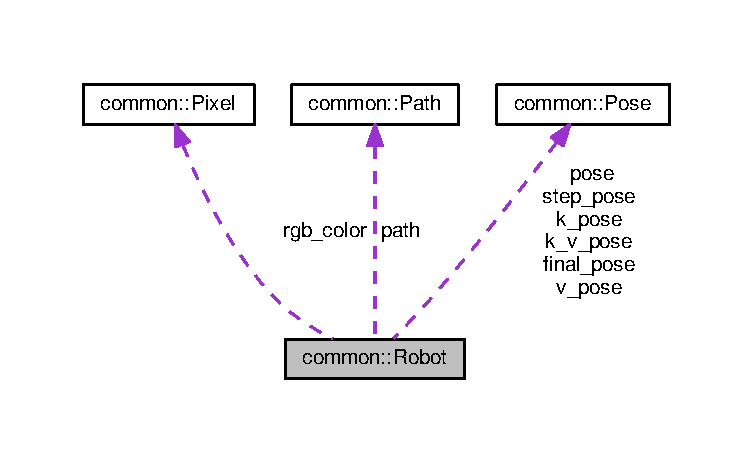
\includegraphics[width=350pt]{structcommon_1_1Robot__coll__graph}
\end{center}
\end{figure}
\subsection*{Métodos Públicos}
\begin{DoxyCompactItemize}
\item 
\hyperlink{structcommon_1_1Robot_a41ba088fd67d929808e381126f7b6c2e}{Robot} ()\hypertarget{structcommon_1_1Robot_a41ba088fd67d929808e381126f7b6c2e}{}\label{structcommon_1_1Robot_a41ba088fd67d929808e381126f7b6c2e}

\begin{DoxyCompactList}\small\item\em Construtor D\+E\+F\+A\+U\+LT. \end{DoxyCompactList}\item 
\hyperlink{structcommon_1_1Robot_a3df83e11a40060ea9d3553384dcdaaa3}{Robot} (\hyperlink{structcommon_1_1Robot}{Robot} $\ast$r)\hypertarget{structcommon_1_1Robot_a3df83e11a40060ea9d3553384dcdaaa3}{}\label{structcommon_1_1Robot_a3df83e11a40060ea9d3553384dcdaaa3}

\begin{DoxyCompactList}\small\item\em Construtor cópia. \end{DoxyCompactList}\item 
void \hyperlink{structcommon_1_1Robot_a224e3f9997e44c5edf67fd0989aee5cf}{show} ()\hypertarget{structcommon_1_1Robot_a224e3f9997e44c5edf67fd0989aee5cf}{}\label{structcommon_1_1Robot_a224e3f9997e44c5edf67fd0989aee5cf}

\begin{DoxyCompactList}\small\item\em Método de debug no terminal. \end{DoxyCompactList}\end{DoxyCompactItemize}
\subsection*{Atributos Públicos}
\begin{DoxyCompactItemize}
\item 
int \hyperlink{structcommon_1_1Robot_a59c0c9960153de3d38d4bbcc479015e3}{id}\hypertarget{structcommon_1_1Robot_a59c0c9960153de3d38d4bbcc479015e3}{}\label{structcommon_1_1Robot_a59c0c9960153de3d38d4bbcc479015e3}

\begin{DoxyCompactList}\small\item\em Id do robô \end{DoxyCompactList}\item 
\hyperlink{structcommon_1_1Pose}{Pose} \hyperlink{structcommon_1_1Robot_a9b7add6f5e5486d5d9bab91ab1800225}{pose}\hypertarget{structcommon_1_1Robot_a9b7add6f5e5486d5d9bab91ab1800225}{}\label{structcommon_1_1Robot_a9b7add6f5e5486d5d9bab91ab1800225}

\begin{DoxyCompactList}\small\item\em \hyperlink{structcommon_1_1Pose}{Pose} de um robô no campo. \end{DoxyCompactList}\item 
\hyperlink{structcommon_1_1Pose}{Pose} \hyperlink{structcommon_1_1Robot_a76821833979c7bca183906c74d383d7d}{v\+\_\+pose}\hypertarget{structcommon_1_1Robot_a76821833979c7bca183906c74d383d7d}{}\label{structcommon_1_1Robot_a76821833979c7bca183906c74d383d7d}

\begin{DoxyCompactList}\small\item\em Velocidades linear, tangencial e angular de um robô no campo. \end{DoxyCompactList}\item 
\hyperlink{structcommon_1_1Pose}{Pose} \hyperlink{structcommon_1_1Robot_a33dcdc52395edee9f7e27fa609eedeb2}{k\+\_\+pose}\hypertarget{structcommon_1_1Robot_a33dcdc52395edee9f7e27fa609eedeb2}{}\label{structcommon_1_1Robot_a33dcdc52395edee9f7e27fa609eedeb2}

\begin{DoxyCompactList}\small\item\em Estimação da pose do robô pelo filtro de kalman. Utilizado somente com pacote vindo do V\+S\+S-\/\+Vision. \end{DoxyCompactList}\item 
\hyperlink{structcommon_1_1Pose}{Pose} \hyperlink{structcommon_1_1Robot_a1f76a8c236dbaa91e16f1d02c0340be9}{k\+\_\+v\+\_\+pose}\hypertarget{structcommon_1_1Robot_a1f76a8c236dbaa91e16f1d02c0340be9}{}\label{structcommon_1_1Robot_a1f76a8c236dbaa91e16f1d02c0340be9}

\begin{DoxyCompactList}\small\item\em Estimação das velocidades linear, tangencial e angular pelo filtro de kalman. Utilizado somente com pacote vindo do V\+S\+S-\/\+Vision. \end{DoxyCompactList}\item 
\hyperlink{structcommon_1_1Pose}{Pose} \hyperlink{structcommon_1_1Robot_a5331036a164340832f703b81e834711e}{step\+\_\+pose}\hypertarget{structcommon_1_1Robot_a5331036a164340832f703b81e834711e}{}\label{structcommon_1_1Robot_a5331036a164340832f703b81e834711e}

\begin{DoxyCompactList}\small\item\em Vetor de movimentação, isto é, para onde o robô irá \end{DoxyCompactList}\item 
\hyperlink{structcommon_1_1Pose}{Pose} \hyperlink{structcommon_1_1Robot_a5b2cbd0f64426838b76365fee4f2cd7f}{final\+\_\+pose}\hypertarget{structcommon_1_1Robot_a5b2cbd0f64426838b76365fee4f2cd7f}{}\label{structcommon_1_1Robot_a5b2cbd0f64426838b76365fee4f2cd7f}

\begin{DoxyCompactList}\small\item\em \hyperlink{structcommon_1_1Pose}{Pose} final do robô \end{DoxyCompactList}\item 
\hyperlink{structcommon_1_1Path}{Path} \hyperlink{structcommon_1_1Robot_a7c07b8d76466e74162a77cb4245e7051}{path}\hypertarget{structcommon_1_1Robot_a7c07b8d76466e74162a77cb4245e7051}{}\label{structcommon_1_1Robot_a7c07b8d76466e74162a77cb4245e7051}

\begin{DoxyCompactList}\small\item\em Caminho que um robô irá executar. \end{DoxyCompactList}\item 
int \hyperlink{structcommon_1_1Robot_a4f69dbd752e60a34b7f87d779e31ae74}{team}\hypertarget{structcommon_1_1Robot_a4f69dbd752e60a34b7f87d779e31ae74}{}\label{structcommon_1_1Robot_a4f69dbd752e60a34b7f87d779e31ae74}

\begin{DoxyCompactList}\small\item\em Id do time\+: 0 = amarelo, 1 = azul. \end{DoxyCompactList}\item 
int \hyperlink{structcommon_1_1Robot_a1fc861b50fde0ea004276db69be5026d}{color}\hypertarget{structcommon_1_1Robot_a1fc861b50fde0ea004276db69be5026d}{}\label{structcommon_1_1Robot_a1fc861b50fde0ea004276db69be5026d}

\begin{DoxyCompactList}\small\item\em Cor do robô, com base no enum de cores. Utilizado com o V\+S\+S-\/\+Simulator. \end{DoxyCompactList}\item 
\hyperlink{structcommon_1_1Pixel}{Pixel} \hyperlink{structcommon_1_1Robot_af2c38313d74d1b710b260e5ac903fab9}{rgb\+\_\+color}\hypertarget{structcommon_1_1Robot_af2c38313d74d1b710b260e5ac903fab9}{}\label{structcommon_1_1Robot_af2c38313d74d1b710b260e5ac903fab9}

\begin{DoxyCompactList}\small\item\em Cor do robô, com base no valor R\+GB. Utilizado com o V\+S\+S-\/\+Vision. \end{DoxyCompactList}\item 
int \hyperlink{structcommon_1_1Robot_a5f8ee844a4dc4a86d30a41c2a4100bfa}{team\+\_\+label}\hypertarget{structcommon_1_1Robot_a5f8ee844a4dc4a86d30a41c2a4100bfa}{}\label{structcommon_1_1Robot_a5f8ee844a4dc4a86d30a41c2a4100bfa}

\begin{DoxyCompactList}\small\item\em T\+O\+DO. \end{DoxyCompactList}\item 
int \hyperlink{structcommon_1_1Robot_a26877803f1772bb5cd5b0fabe8a9ee99}{color\+\_\+label}\hypertarget{structcommon_1_1Robot_a26877803f1772bb5cd5b0fabe8a9ee99}{}\label{structcommon_1_1Robot_a26877803f1772bb5cd5b0fabe8a9ee99}

\begin{DoxyCompactList}\small\item\em T\+O\+DO. \end{DoxyCompactList}\item 
float \hyperlink{structcommon_1_1Robot_a45485c8807aa375d14b7808ffef4adde}{radius}\hypertarget{structcommon_1_1Robot_a45485c8807aa375d14b7808ffef4adde}{}\label{structcommon_1_1Robot_a45485c8807aa375d14b7808ffef4adde}

\begin{DoxyCompactList}\small\item\em Raio do robô \end{DoxyCompactList}\item 
bool \hyperlink{structcommon_1_1Robot_a791ca826eed1f0ef29d5df539fdb2dad}{has\+\_\+step}\hypertarget{structcommon_1_1Robot_a791ca826eed1f0ef29d5df539fdb2dad}{}\label{structcommon_1_1Robot_a791ca826eed1f0ef29d5df539fdb2dad}

\begin{DoxyCompactList}\small\item\em Booleano que define se o pacote de debug possui um vetor de movimentação. \end{DoxyCompactList}\item 
bool \hyperlink{structcommon_1_1Robot_a53ef950d28fe6fb46c21af2c0bf5eba0}{has\+\_\+final}\hypertarget{structcommon_1_1Robot_a53ef950d28fe6fb46c21af2c0bf5eba0}{}\label{structcommon_1_1Robot_a53ef950d28fe6fb46c21af2c0bf5eba0}

\begin{DoxyCompactList}\small\item\em Booleano que define se o pacote de debug possui uma pose final. \end{DoxyCompactList}\end{DoxyCompactItemize}


\subsection{Descrição Detalhada}
Essa struct é responsável por representar um robô 

A documentação para esta estrutura foi gerada a partir do seguinte arquivo\+:\begin{DoxyCompactItemize}
\item 
/home/johnathan/\+Repositories/\+S\+I\+R\+Lab/\+Public/\+V\+S\+S-\/\+Viewer/src/commons.\+h\end{DoxyCompactItemize}

\hypertarget{classvss__command_1_1Robot__Command}{}\section{Referência da Classe vss\+\_\+command\+:\+:Robot\+\_\+\+Command}
\label{classvss__command_1_1Robot__Command}\index{vss\+\_\+command\+::\+Robot\+\_\+\+Command@{vss\+\_\+command\+::\+Robot\+\_\+\+Command}}


Diagrama de Hierarquia para vss\+\_\+command\+:\+:Robot\+\_\+\+Command\+:\nopagebreak
\begin{figure}[H]
\begin{center}
\leavevmode
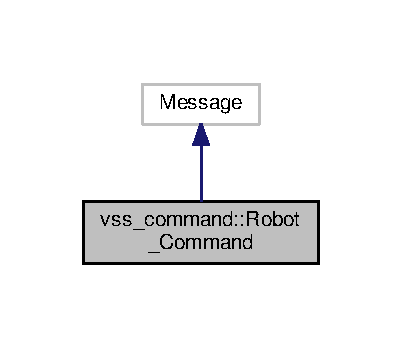
\includegraphics[width=193pt]{classvss__command_1_1Robot__Command__inherit__graph}
\end{center}
\end{figure}


Diagrama de colaboração para vss\+\_\+command\+:\+:Robot\+\_\+\+Command\+:\nopagebreak
\begin{figure}[H]
\begin{center}
\leavevmode
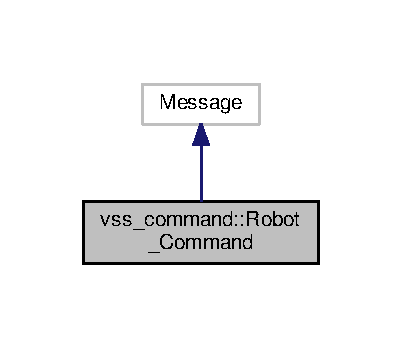
\includegraphics[width=193pt]{classvss__command_1_1Robot__Command__coll__graph}
\end{center}
\end{figure}
\subsection*{Métodos Públicos}
\begin{DoxyCompactItemize}
\item 
{\bfseries Robot\+\_\+\+Command} (const \hyperlink{classvss__command_1_1Robot__Command}{Robot\+\_\+\+Command} \&from)\hypertarget{classvss__command_1_1Robot__Command_aec1028695262ac9887a661768f2f8bb1}{}\label{classvss__command_1_1Robot__Command_aec1028695262ac9887a661768f2f8bb1}

\item 
\hyperlink{classvss__command_1_1Robot__Command}{Robot\+\_\+\+Command} \& {\bfseries operator=} (const \hyperlink{classvss__command_1_1Robot__Command}{Robot\+\_\+\+Command} \&from)\hypertarget{classvss__command_1_1Robot__Command_afebc3c2ee761027356ce0fabe568ae11}{}\label{classvss__command_1_1Robot__Command_afebc3c2ee761027356ce0fabe568ae11}

\item 
const \+::google\+::protobuf\+::\+Unknown\+Field\+Set \& {\bfseries unknown\+\_\+fields} () const \hypertarget{classvss__command_1_1Robot__Command_a9df4b6bca5721e6b1ae945dc975af2c6}{}\label{classvss__command_1_1Robot__Command_a9df4b6bca5721e6b1ae945dc975af2c6}

\item 
inline\+::google\+::protobuf\+::\+Unknown\+Field\+Set $\ast$ {\bfseries mutable\+\_\+unknown\+\_\+fields} ()\hypertarget{classvss__command_1_1Robot__Command_ac59c88c8dcf9b0e1128e845e238a92d4}{}\label{classvss__command_1_1Robot__Command_ac59c88c8dcf9b0e1128e845e238a92d4}

\item 
void {\bfseries Swap} (\hyperlink{classvss__command_1_1Robot__Command}{Robot\+\_\+\+Command} $\ast$other)\hypertarget{classvss__command_1_1Robot__Command_aab4cd2f4e6d3316f414fa32e7ccf1660}{}\label{classvss__command_1_1Robot__Command_aab4cd2f4e6d3316f414fa32e7ccf1660}

\item 
\hyperlink{classvss__command_1_1Robot__Command}{Robot\+\_\+\+Command} $\ast$ {\bfseries New} () const \hypertarget{classvss__command_1_1Robot__Command_a2a1745c8adfb0fc0fe73449b980ecbee}{}\label{classvss__command_1_1Robot__Command_a2a1745c8adfb0fc0fe73449b980ecbee}

\item 
\hyperlink{classvss__command_1_1Robot__Command}{Robot\+\_\+\+Command} $\ast$ {\bfseries New} (\+::google\+::protobuf\+::\+Arena $\ast$arena) const \hypertarget{classvss__command_1_1Robot__Command_a27964fb97280ed66c14729fec9f545d2}{}\label{classvss__command_1_1Robot__Command_a27964fb97280ed66c14729fec9f545d2}

\item 
void {\bfseries Copy\+From} (const \+::google\+::protobuf\+::\+Message \&from)\hypertarget{classvss__command_1_1Robot__Command_a44b1cba95f68eb9c9349d1f06b0567db}{}\label{classvss__command_1_1Robot__Command_a44b1cba95f68eb9c9349d1f06b0567db}

\item 
void {\bfseries Merge\+From} (const \+::google\+::protobuf\+::\+Message \&from)\hypertarget{classvss__command_1_1Robot__Command_a72b9a2f6e5fcb0ee33f5c1a5782bb655}{}\label{classvss__command_1_1Robot__Command_a72b9a2f6e5fcb0ee33f5c1a5782bb655}

\item 
void {\bfseries Copy\+From} (const \hyperlink{classvss__command_1_1Robot__Command}{Robot\+\_\+\+Command} \&from)\hypertarget{classvss__command_1_1Robot__Command_a98f8965b27b6495b2d59dccd8d2bfe19}{}\label{classvss__command_1_1Robot__Command_a98f8965b27b6495b2d59dccd8d2bfe19}

\item 
void {\bfseries Merge\+From} (const \hyperlink{classvss__command_1_1Robot__Command}{Robot\+\_\+\+Command} \&from)\hypertarget{classvss__command_1_1Robot__Command_a48c5d39a8a3d31209db79aa77fcf876f}{}\label{classvss__command_1_1Robot__Command_a48c5d39a8a3d31209db79aa77fcf876f}

\item 
void {\bfseries Clear} ()\hypertarget{classvss__command_1_1Robot__Command_aaffa12def3a1311252dcaccf6becb28b}{}\label{classvss__command_1_1Robot__Command_aaffa12def3a1311252dcaccf6becb28b}

\item 
bool {\bfseries Is\+Initialized} () const \hypertarget{classvss__command_1_1Robot__Command_af368ddcdb8103f40b21503727664fc52}{}\label{classvss__command_1_1Robot__Command_af368ddcdb8103f40b21503727664fc52}

\item 
int {\bfseries Byte\+Size} () const \hypertarget{classvss__command_1_1Robot__Command_a54599973bda6814c7842036eb9bf9229}{}\label{classvss__command_1_1Robot__Command_a54599973bda6814c7842036eb9bf9229}

\item 
bool {\bfseries Merge\+Partial\+From\+Coded\+Stream} (\+::google\+::protobuf\+::io\+::\+Coded\+Input\+Stream $\ast$input)\hypertarget{classvss__command_1_1Robot__Command_a471b2b99a1e476866bdb6ded82d46274}{}\label{classvss__command_1_1Robot__Command_a471b2b99a1e476866bdb6ded82d46274}

\item 
void {\bfseries Serialize\+With\+Cached\+Sizes} (\+::google\+::protobuf\+::io\+::\+Coded\+Output\+Stream $\ast$output) const \hypertarget{classvss__command_1_1Robot__Command_add920699d3f456d9335a4fbacf4a1fa5}{}\label{classvss__command_1_1Robot__Command_add920699d3f456d9335a4fbacf4a1fa5}

\item 
\+::google\+::protobuf\+::uint8 $\ast$ {\bfseries Internal\+Serialize\+With\+Cached\+Sizes\+To\+Array} (bool deterministic,\+::google\+::protobuf\+::uint8 $\ast$output) const \hypertarget{classvss__command_1_1Robot__Command_a4ab1a2204defe3b1c6930b295607f00d}{}\label{classvss__command_1_1Robot__Command_a4ab1a2204defe3b1c6930b295607f00d}

\item 
\+::google\+::protobuf\+::uint8 $\ast$ {\bfseries Serialize\+With\+Cached\+Sizes\+To\+Array} (\+::google\+::protobuf\+::uint8 $\ast$output) const \hypertarget{classvss__command_1_1Robot__Command_aaa2b9a287b4ac50966156dbca7ec50e1}{}\label{classvss__command_1_1Robot__Command_aaa2b9a287b4ac50966156dbca7ec50e1}

\item 
int {\bfseries Get\+Cached\+Size} () const \hypertarget{classvss__command_1_1Robot__Command_a45dc66dc5c38e988073141707b083dae}{}\label{classvss__command_1_1Robot__Command_a45dc66dc5c38e988073141707b083dae}

\item 
\+::google\+::protobuf\+::\+Metadata {\bfseries Get\+Metadata} () const \hypertarget{classvss__command_1_1Robot__Command_a5383c49b5b6ef83dc3b9ac3ab2dd870a}{}\label{classvss__command_1_1Robot__Command_a5383c49b5b6ef83dc3b9ac3ab2dd870a}

\item 
bool {\bfseries has\+\_\+id} () const \hypertarget{classvss__command_1_1Robot__Command_ab636015fe88af27ccaf824159805442d}{}\label{classvss__command_1_1Robot__Command_ab636015fe88af27ccaf824159805442d}

\item 
void {\bfseries clear\+\_\+id} ()\hypertarget{classvss__command_1_1Robot__Command_a0b684f61267d6e251f068f1b2a4c772f}{}\label{classvss__command_1_1Robot__Command_a0b684f61267d6e251f068f1b2a4c772f}

\item 
\+::google\+::protobuf\+::uint32 {\bfseries id} () const \hypertarget{classvss__command_1_1Robot__Command_a632b1e7c37152ca3ecca6e45547faa94}{}\label{classvss__command_1_1Robot__Command_a632b1e7c37152ca3ecca6e45547faa94}

\item 
void {\bfseries set\+\_\+id} (\+::google\+::protobuf\+::uint32 value)\hypertarget{classvss__command_1_1Robot__Command_a7aa38699c29bd2037112084fbb833efe}{}\label{classvss__command_1_1Robot__Command_a7aa38699c29bd2037112084fbb833efe}

\item 
bool {\bfseries has\+\_\+left\+\_\+vel} () const \hypertarget{classvss__command_1_1Robot__Command_aba5afdfa1c9844cbea2b8b5c1f9a3a71}{}\label{classvss__command_1_1Robot__Command_aba5afdfa1c9844cbea2b8b5c1f9a3a71}

\item 
void {\bfseries clear\+\_\+left\+\_\+vel} ()\hypertarget{classvss__command_1_1Robot__Command_a728166b3b1a62583a6e46545b5ad44c7}{}\label{classvss__command_1_1Robot__Command_a728166b3b1a62583a6e46545b5ad44c7}

\item 
float {\bfseries left\+\_\+vel} () const \hypertarget{classvss__command_1_1Robot__Command_a179ef683cadb10827e8112f2f1e174a5}{}\label{classvss__command_1_1Robot__Command_a179ef683cadb10827e8112f2f1e174a5}

\item 
void {\bfseries set\+\_\+left\+\_\+vel} (float value)\hypertarget{classvss__command_1_1Robot__Command_a2792ed641e6a25348fab7d26d989f670}{}\label{classvss__command_1_1Robot__Command_a2792ed641e6a25348fab7d26d989f670}

\item 
bool {\bfseries has\+\_\+right\+\_\+vel} () const \hypertarget{classvss__command_1_1Robot__Command_af192678ad6c73ff034b042275511d503}{}\label{classvss__command_1_1Robot__Command_af192678ad6c73ff034b042275511d503}

\item 
void {\bfseries clear\+\_\+right\+\_\+vel} ()\hypertarget{classvss__command_1_1Robot__Command_acdb3ec06b0b7183f192df01af72e70aa}{}\label{classvss__command_1_1Robot__Command_acdb3ec06b0b7183f192df01af72e70aa}

\item 
float {\bfseries right\+\_\+vel} () const \hypertarget{classvss__command_1_1Robot__Command_ad8e37a453b8729183b59a2bade49cc74}{}\label{classvss__command_1_1Robot__Command_ad8e37a453b8729183b59a2bade49cc74}

\item 
void {\bfseries set\+\_\+right\+\_\+vel} (float value)\hypertarget{classvss__command_1_1Robot__Command_a6e63f0df3268bde40f11d47ea167ceb3}{}\label{classvss__command_1_1Robot__Command_a6e63f0df3268bde40f11d47ea167ceb3}

\end{DoxyCompactItemize}
\subsection*{Métodos Públicos Estáticos}
\begin{DoxyCompactItemize}
\item 
static const \+::google\+::protobuf\+::\+Descriptor $\ast$ {\bfseries descriptor} ()\hypertarget{classvss__command_1_1Robot__Command_ad40c6b295898b078ff34e9966d89b6e5}{}\label{classvss__command_1_1Robot__Command_ad40c6b295898b078ff34e9966d89b6e5}

\item 
static const \hyperlink{classvss__command_1_1Robot__Command}{Robot\+\_\+\+Command} \& {\bfseries default\+\_\+instance} ()\hypertarget{classvss__command_1_1Robot__Command_a4c818a68a4bee11acbc7e7b5483ff4d7}{}\label{classvss__command_1_1Robot__Command_a4c818a68a4bee11acbc7e7b5483ff4d7}

\end{DoxyCompactItemize}
\subsection*{Atributos Estáticos Públicos}
\begin{DoxyCompactItemize}
\item 
static const int {\bfseries k\+Id\+Field\+Number} = 1\hypertarget{classvss__command_1_1Robot__Command_a72d358bc06840eb9b5835ad46cee4620}{}\label{classvss__command_1_1Robot__Command_a72d358bc06840eb9b5835ad46cee4620}

\item 
static const int {\bfseries k\+Left\+Vel\+Field\+Number} = 2\hypertarget{classvss__command_1_1Robot__Command_a834467a27672508216892c745d78bad4}{}\label{classvss__command_1_1Robot__Command_a834467a27672508216892c745d78bad4}

\item 
static const int {\bfseries k\+Right\+Vel\+Field\+Number} = 3\hypertarget{classvss__command_1_1Robot__Command_adb4e9f137218f7bf68ba93029e028e40}{}\label{classvss__command_1_1Robot__Command_adb4e9f137218f7bf68ba93029e028e40}

\end{DoxyCompactItemize}
\subsection*{Amigas}
\begin{DoxyCompactItemize}
\item 
void {\bfseries protobuf\+\_\+\+Add\+Desc\+\_\+command\+\_\+2eproto} ()\hypertarget{classvss__command_1_1Robot__Command_a4825d92f856fcb4b02c67b601c433796}{}\label{classvss__command_1_1Robot__Command_a4825d92f856fcb4b02c67b601c433796}

\item 
void {\bfseries protobuf\+\_\+\+Assign\+Desc\+\_\+command\+\_\+2eproto} ()\hypertarget{classvss__command_1_1Robot__Command_a4c6fb97c25079d49daf010087d869100}{}\label{classvss__command_1_1Robot__Command_a4c6fb97c25079d49daf010087d869100}

\item 
void {\bfseries protobuf\+\_\+\+Shutdown\+File\+\_\+command\+\_\+2eproto} ()\hypertarget{classvss__command_1_1Robot__Command_a4cf10633ad46690f5eec6bdbbcf62de0}{}\label{classvss__command_1_1Robot__Command_a4cf10633ad46690f5eec6bdbbcf62de0}

\end{DoxyCompactItemize}


A documentação para esta classe foi gerada a partir dos seguintes arquivos\+:\begin{DoxyCompactItemize}
\item 
/home/johnathan/\+Repositories/\+S\+I\+R\+Lab/\+Projects/\+V\+S\+S-\/\+Viewer/src/\+V\+S\+S-\/\+Interface/protos/command.\+pb.\+h\item 
/home/johnathan/\+Repositories/\+S\+I\+R\+Lab/\+Projects/\+V\+S\+S-\/\+Viewer/src/\+V\+S\+S-\/\+Interface/protos/command.\+pb.\+cc\end{DoxyCompactItemize}

\hypertarget{classvss__state_1_1Robot__State}{}\section{Referência da Classe vss\+\_\+state\+:\+:Robot\+\_\+\+State}
\label{classvss__state_1_1Robot__State}\index{vss\+\_\+state\+::\+Robot\+\_\+\+State@{vss\+\_\+state\+::\+Robot\+\_\+\+State}}


Diagrama de Hierarquia para vss\+\_\+state\+:\+:Robot\+\_\+\+State\+:\nopagebreak
\begin{figure}[H]
\begin{center}
\leavevmode
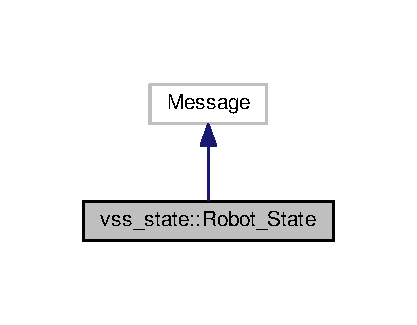
\includegraphics[width=200pt]{classvss__state_1_1Robot__State__inherit__graph}
\end{center}
\end{figure}


Diagrama de colaboração para vss\+\_\+state\+:\+:Robot\+\_\+\+State\+:\nopagebreak
\begin{figure}[H]
\begin{center}
\leavevmode
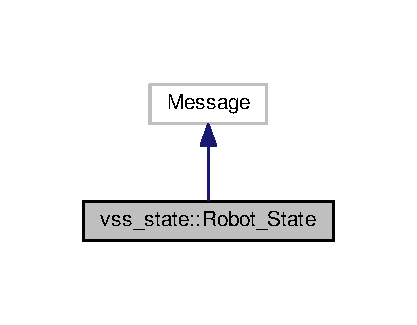
\includegraphics[width=200pt]{classvss__state_1_1Robot__State__coll__graph}
\end{center}
\end{figure}
\subsection*{Métodos Públicos}
\begin{DoxyCompactItemize}
\item 
{\bfseries Robot\+\_\+\+State} (const \hyperlink{classvss__state_1_1Robot__State}{Robot\+\_\+\+State} \&from)\hypertarget{classvss__state_1_1Robot__State_a067b968ee504ea53efd93d9aa27c96ca}{}\label{classvss__state_1_1Robot__State_a067b968ee504ea53efd93d9aa27c96ca}

\item 
\hyperlink{classvss__state_1_1Robot__State}{Robot\+\_\+\+State} \& {\bfseries operator=} (const \hyperlink{classvss__state_1_1Robot__State}{Robot\+\_\+\+State} \&from)\hypertarget{classvss__state_1_1Robot__State_ad37aa84870eea581e0406cfb5db502ac}{}\label{classvss__state_1_1Robot__State_ad37aa84870eea581e0406cfb5db502ac}

\item 
const \+::google\+::protobuf\+::\+Unknown\+Field\+Set \& {\bfseries unknown\+\_\+fields} () const \hypertarget{classvss__state_1_1Robot__State_a12a57833a931bfb941527d777fb1d99a}{}\label{classvss__state_1_1Robot__State_a12a57833a931bfb941527d777fb1d99a}

\item 
inline\+::google\+::protobuf\+::\+Unknown\+Field\+Set $\ast$ {\bfseries mutable\+\_\+unknown\+\_\+fields} ()\hypertarget{classvss__state_1_1Robot__State_adda3db07f10ebdb69699bb992976ace3}{}\label{classvss__state_1_1Robot__State_adda3db07f10ebdb69699bb992976ace3}

\item 
void {\bfseries Swap} (\hyperlink{classvss__state_1_1Robot__State}{Robot\+\_\+\+State} $\ast$other)\hypertarget{classvss__state_1_1Robot__State_a4f0475b13ab71a00c88f4662e82decea}{}\label{classvss__state_1_1Robot__State_a4f0475b13ab71a00c88f4662e82decea}

\item 
\hyperlink{classvss__state_1_1Robot__State}{Robot\+\_\+\+State} $\ast$ {\bfseries New} () const \hypertarget{classvss__state_1_1Robot__State_ac7c2f86026d390635f40306421511edd}{}\label{classvss__state_1_1Robot__State_ac7c2f86026d390635f40306421511edd}

\item 
\hyperlink{classvss__state_1_1Robot__State}{Robot\+\_\+\+State} $\ast$ {\bfseries New} (\+::google\+::protobuf\+::\+Arena $\ast$arena) const \hypertarget{classvss__state_1_1Robot__State_aa802503ef36b7df6e88c544913d9cc43}{}\label{classvss__state_1_1Robot__State_aa802503ef36b7df6e88c544913d9cc43}

\item 
void {\bfseries Copy\+From} (const \+::google\+::protobuf\+::\+Message \&from)\hypertarget{classvss__state_1_1Robot__State_ad8ff7bd295e28703ef3b6bdc6dba1435}{}\label{classvss__state_1_1Robot__State_ad8ff7bd295e28703ef3b6bdc6dba1435}

\item 
void {\bfseries Merge\+From} (const \+::google\+::protobuf\+::\+Message \&from)\hypertarget{classvss__state_1_1Robot__State_a5f5cb63411c8f37399dfd169c94e6e54}{}\label{classvss__state_1_1Robot__State_a5f5cb63411c8f37399dfd169c94e6e54}

\item 
void {\bfseries Copy\+From} (const \hyperlink{classvss__state_1_1Robot__State}{Robot\+\_\+\+State} \&from)\hypertarget{classvss__state_1_1Robot__State_a4e18e564b9c470d6f382c8c1c040cfb4}{}\label{classvss__state_1_1Robot__State_a4e18e564b9c470d6f382c8c1c040cfb4}

\item 
void {\bfseries Merge\+From} (const \hyperlink{classvss__state_1_1Robot__State}{Robot\+\_\+\+State} \&from)\hypertarget{classvss__state_1_1Robot__State_a66fadfccfb89ba8742bafa6cd9597420}{}\label{classvss__state_1_1Robot__State_a66fadfccfb89ba8742bafa6cd9597420}

\item 
void {\bfseries Clear} ()\hypertarget{classvss__state_1_1Robot__State_a78f3f24cbb0f2e1fac867550bf05da91}{}\label{classvss__state_1_1Robot__State_a78f3f24cbb0f2e1fac867550bf05da91}

\item 
bool {\bfseries Is\+Initialized} () const \hypertarget{classvss__state_1_1Robot__State_ae482d98ba51e51887efe37a4d2f6abb5}{}\label{classvss__state_1_1Robot__State_ae482d98ba51e51887efe37a4d2f6abb5}

\item 
int {\bfseries Byte\+Size} () const \hypertarget{classvss__state_1_1Robot__State_a6ff13cd34434ab985d2b560a13219532}{}\label{classvss__state_1_1Robot__State_a6ff13cd34434ab985d2b560a13219532}

\item 
bool {\bfseries Merge\+Partial\+From\+Coded\+Stream} (\+::google\+::protobuf\+::io\+::\+Coded\+Input\+Stream $\ast$input)\hypertarget{classvss__state_1_1Robot__State_a82a0f5270a13c5211d94c6da6726ab8d}{}\label{classvss__state_1_1Robot__State_a82a0f5270a13c5211d94c6da6726ab8d}

\item 
void {\bfseries Serialize\+With\+Cached\+Sizes} (\+::google\+::protobuf\+::io\+::\+Coded\+Output\+Stream $\ast$output) const \hypertarget{classvss__state_1_1Robot__State_a67b812e24a55cdfad4d58049f8e0e674}{}\label{classvss__state_1_1Robot__State_a67b812e24a55cdfad4d58049f8e0e674}

\item 
\+::google\+::protobuf\+::uint8 $\ast$ {\bfseries Internal\+Serialize\+With\+Cached\+Sizes\+To\+Array} (bool deterministic,\+::google\+::protobuf\+::uint8 $\ast$output) const \hypertarget{classvss__state_1_1Robot__State_a4674117e4328f6b8378b2ea0c6f984a3}{}\label{classvss__state_1_1Robot__State_a4674117e4328f6b8378b2ea0c6f984a3}

\item 
\+::google\+::protobuf\+::uint8 $\ast$ {\bfseries Serialize\+With\+Cached\+Sizes\+To\+Array} (\+::google\+::protobuf\+::uint8 $\ast$output) const \hypertarget{classvss__state_1_1Robot__State_aba509d6681cb9d6a01f2a0ecb65bb613}{}\label{classvss__state_1_1Robot__State_aba509d6681cb9d6a01f2a0ecb65bb613}

\item 
int {\bfseries Get\+Cached\+Size} () const \hypertarget{classvss__state_1_1Robot__State_ada89e91697c3773ab009c765b2884734}{}\label{classvss__state_1_1Robot__State_ada89e91697c3773ab009c765b2884734}

\item 
\+::google\+::protobuf\+::\+Metadata {\bfseries Get\+Metadata} () const \hypertarget{classvss__state_1_1Robot__State_afb2668f8b861828a30ac978ab416e900}{}\label{classvss__state_1_1Robot__State_afb2668f8b861828a30ac978ab416e900}

\item 
bool {\bfseries has\+\_\+pose} () const \hypertarget{classvss__state_1_1Robot__State_a16f5802d6a727b0c4c98472010c12460}{}\label{classvss__state_1_1Robot__State_a16f5802d6a727b0c4c98472010c12460}

\item 
void {\bfseries clear\+\_\+pose} ()\hypertarget{classvss__state_1_1Robot__State_a33d40f6cc351a111c3bae3e095566564}{}\label{classvss__state_1_1Robot__State_a33d40f6cc351a111c3bae3e095566564}

\item 
const \+::\hyperlink{classvss__state_1_1Pose}{vss\+\_\+state\+::\+Pose} \& {\bfseries pose} () const \hypertarget{classvss__state_1_1Robot__State_a0c7dee60f0d9b34d6708f7912e666e68}{}\label{classvss__state_1_1Robot__State_a0c7dee60f0d9b34d6708f7912e666e68}

\item 
\+::\hyperlink{classvss__state_1_1Pose}{vss\+\_\+state\+::\+Pose} $\ast$ {\bfseries mutable\+\_\+pose} ()\hypertarget{classvss__state_1_1Robot__State_a08d3b0444895130052a1805120013941}{}\label{classvss__state_1_1Robot__State_a08d3b0444895130052a1805120013941}

\item 
\+::\hyperlink{classvss__state_1_1Pose}{vss\+\_\+state\+::\+Pose} $\ast$ {\bfseries release\+\_\+pose} ()\hypertarget{classvss__state_1_1Robot__State_ad644f3a9823f0cf600305257b0608b46}{}\label{classvss__state_1_1Robot__State_ad644f3a9823f0cf600305257b0608b46}

\item 
void {\bfseries set\+\_\+allocated\+\_\+pose} (\+::\hyperlink{classvss__state_1_1Pose}{vss\+\_\+state\+::\+Pose} $\ast$pose)\hypertarget{classvss__state_1_1Robot__State_af8564fc0f0e930796b9ba74fbf02b057}{}\label{classvss__state_1_1Robot__State_af8564fc0f0e930796b9ba74fbf02b057}

\item 
bool {\bfseries has\+\_\+v\+\_\+pose} () const \hypertarget{classvss__state_1_1Robot__State_a99a2138f4352bfac49f101ef1a3e2aa3}{}\label{classvss__state_1_1Robot__State_a99a2138f4352bfac49f101ef1a3e2aa3}

\item 
void {\bfseries clear\+\_\+v\+\_\+pose} ()\hypertarget{classvss__state_1_1Robot__State_ad7bb63ae44945655a400d71825c4e6cc}{}\label{classvss__state_1_1Robot__State_ad7bb63ae44945655a400d71825c4e6cc}

\item 
const \+::\hyperlink{classvss__state_1_1Pose}{vss\+\_\+state\+::\+Pose} \& {\bfseries v\+\_\+pose} () const \hypertarget{classvss__state_1_1Robot__State_af05253d869ead02f02a8ea56f0ec989f}{}\label{classvss__state_1_1Robot__State_af05253d869ead02f02a8ea56f0ec989f}

\item 
\+::\hyperlink{classvss__state_1_1Pose}{vss\+\_\+state\+::\+Pose} $\ast$ {\bfseries mutable\+\_\+v\+\_\+pose} ()\hypertarget{classvss__state_1_1Robot__State_ad5bd41bfe20e17c7c35a1cd91ff24a4a}{}\label{classvss__state_1_1Robot__State_ad5bd41bfe20e17c7c35a1cd91ff24a4a}

\item 
\+::\hyperlink{classvss__state_1_1Pose}{vss\+\_\+state\+::\+Pose} $\ast$ {\bfseries release\+\_\+v\+\_\+pose} ()\hypertarget{classvss__state_1_1Robot__State_a1d4e9041543747c034f54d98fd952d6e}{}\label{classvss__state_1_1Robot__State_a1d4e9041543747c034f54d98fd952d6e}

\item 
void {\bfseries set\+\_\+allocated\+\_\+v\+\_\+pose} (\+::\hyperlink{classvss__state_1_1Pose}{vss\+\_\+state\+::\+Pose} $\ast$v\+\_\+pose)\hypertarget{classvss__state_1_1Robot__State_a4e979918840ca68e80f7f602341ed766}{}\label{classvss__state_1_1Robot__State_a4e979918840ca68e80f7f602341ed766}

\item 
bool {\bfseries has\+\_\+k\+\_\+pose} () const \hypertarget{classvss__state_1_1Robot__State_a7754831605dadf0fa81b739f1ebf920d}{}\label{classvss__state_1_1Robot__State_a7754831605dadf0fa81b739f1ebf920d}

\item 
void {\bfseries clear\+\_\+k\+\_\+pose} ()\hypertarget{classvss__state_1_1Robot__State_a1adc3e3ef2845d0da77660cc3879969c}{}\label{classvss__state_1_1Robot__State_a1adc3e3ef2845d0da77660cc3879969c}

\item 
const \+::\hyperlink{classvss__state_1_1Pose}{vss\+\_\+state\+::\+Pose} \& {\bfseries k\+\_\+pose} () const \hypertarget{classvss__state_1_1Robot__State_a35253ee22b61da81e9bca8d0c3f338fc}{}\label{classvss__state_1_1Robot__State_a35253ee22b61da81e9bca8d0c3f338fc}

\item 
\+::\hyperlink{classvss__state_1_1Pose}{vss\+\_\+state\+::\+Pose} $\ast$ {\bfseries mutable\+\_\+k\+\_\+pose} ()\hypertarget{classvss__state_1_1Robot__State_ac807165c96cb5b59ae5341cc46f38996}{}\label{classvss__state_1_1Robot__State_ac807165c96cb5b59ae5341cc46f38996}

\item 
\+::\hyperlink{classvss__state_1_1Pose}{vss\+\_\+state\+::\+Pose} $\ast$ {\bfseries release\+\_\+k\+\_\+pose} ()\hypertarget{classvss__state_1_1Robot__State_aadc71d6c4cdd034e934ad365e333f11c}{}\label{classvss__state_1_1Robot__State_aadc71d6c4cdd034e934ad365e333f11c}

\item 
void {\bfseries set\+\_\+allocated\+\_\+k\+\_\+pose} (\+::\hyperlink{classvss__state_1_1Pose}{vss\+\_\+state\+::\+Pose} $\ast$k\+\_\+pose)\hypertarget{classvss__state_1_1Robot__State_a4d69689931c42cfc30b748e267674d99}{}\label{classvss__state_1_1Robot__State_a4d69689931c42cfc30b748e267674d99}

\item 
bool {\bfseries has\+\_\+k\+\_\+v\+\_\+pose} () const \hypertarget{classvss__state_1_1Robot__State_a9a83b1c1730126c70d7d9e72bd9309b8}{}\label{classvss__state_1_1Robot__State_a9a83b1c1730126c70d7d9e72bd9309b8}

\item 
void {\bfseries clear\+\_\+k\+\_\+v\+\_\+pose} ()\hypertarget{classvss__state_1_1Robot__State_a72c6e0df54535999e45d050ae93e696f}{}\label{classvss__state_1_1Robot__State_a72c6e0df54535999e45d050ae93e696f}

\item 
const \+::\hyperlink{classvss__state_1_1Pose}{vss\+\_\+state\+::\+Pose} \& {\bfseries k\+\_\+v\+\_\+pose} () const \hypertarget{classvss__state_1_1Robot__State_a0a9ad2ef6674cccffbacad19391d04ec}{}\label{classvss__state_1_1Robot__State_a0a9ad2ef6674cccffbacad19391d04ec}

\item 
\+::\hyperlink{classvss__state_1_1Pose}{vss\+\_\+state\+::\+Pose} $\ast$ {\bfseries mutable\+\_\+k\+\_\+v\+\_\+pose} ()\hypertarget{classvss__state_1_1Robot__State_a75c61cf61895be92975d7cbbb96e9a2b}{}\label{classvss__state_1_1Robot__State_a75c61cf61895be92975d7cbbb96e9a2b}

\item 
\+::\hyperlink{classvss__state_1_1Pose}{vss\+\_\+state\+::\+Pose} $\ast$ {\bfseries release\+\_\+k\+\_\+v\+\_\+pose} ()\hypertarget{classvss__state_1_1Robot__State_a2d609ff6aaaa1093aa4fd1194c1e1d9c}{}\label{classvss__state_1_1Robot__State_a2d609ff6aaaa1093aa4fd1194c1e1d9c}

\item 
void {\bfseries set\+\_\+allocated\+\_\+k\+\_\+v\+\_\+pose} (\+::\hyperlink{classvss__state_1_1Pose}{vss\+\_\+state\+::\+Pose} $\ast$k\+\_\+v\+\_\+pose)\hypertarget{classvss__state_1_1Robot__State_adf1f7422433e9fa210b97a3a257dd5d3}{}\label{classvss__state_1_1Robot__State_adf1f7422433e9fa210b97a3a257dd5d3}

\item 
bool {\bfseries has\+\_\+color} () const \hypertarget{classvss__state_1_1Robot__State_a319868975523f46fce84fedda26c478e}{}\label{classvss__state_1_1Robot__State_a319868975523f46fce84fedda26c478e}

\item 
void {\bfseries clear\+\_\+color} ()\hypertarget{classvss__state_1_1Robot__State_a0d95199c67056fd8a0b6bb873d278392}{}\label{classvss__state_1_1Robot__State_a0d95199c67056fd8a0b6bb873d278392}

\item 
const \+::\hyperlink{classvss__state_1_1RGB}{vss\+\_\+state\+::\+R\+GB} \& {\bfseries color} () const \hypertarget{classvss__state_1_1Robot__State_a1e8b02c137ceae1f7a875bdf5371aa91}{}\label{classvss__state_1_1Robot__State_a1e8b02c137ceae1f7a875bdf5371aa91}

\item 
\+::\hyperlink{classvss__state_1_1RGB}{vss\+\_\+state\+::\+R\+GB} $\ast$ {\bfseries mutable\+\_\+color} ()\hypertarget{classvss__state_1_1Robot__State_aa91b85fa199de6f9b4673529f86f1d01}{}\label{classvss__state_1_1Robot__State_aa91b85fa199de6f9b4673529f86f1d01}

\item 
\+::\hyperlink{classvss__state_1_1RGB}{vss\+\_\+state\+::\+R\+GB} $\ast$ {\bfseries release\+\_\+color} ()\hypertarget{classvss__state_1_1Robot__State_aba8a8ff5aa02a978e3ff2e8b6335f0ce}{}\label{classvss__state_1_1Robot__State_aba8a8ff5aa02a978e3ff2e8b6335f0ce}

\item 
void {\bfseries set\+\_\+allocated\+\_\+color} (\+::\hyperlink{classvss__state_1_1RGB}{vss\+\_\+state\+::\+R\+GB} $\ast$color)\hypertarget{classvss__state_1_1Robot__State_a368a1f90ce946cd075aa050885e1e6d3}{}\label{classvss__state_1_1Robot__State_a368a1f90ce946cd075aa050885e1e6d3}

\end{DoxyCompactItemize}
\subsection*{Métodos Públicos Estáticos}
\begin{DoxyCompactItemize}
\item 
static const \+::google\+::protobuf\+::\+Descriptor $\ast$ {\bfseries descriptor} ()\hypertarget{classvss__state_1_1Robot__State_af15c0b33b2edbd683bfb87c76e9b94b7}{}\label{classvss__state_1_1Robot__State_af15c0b33b2edbd683bfb87c76e9b94b7}

\item 
static const \hyperlink{classvss__state_1_1Robot__State}{Robot\+\_\+\+State} \& {\bfseries default\+\_\+instance} ()\hypertarget{classvss__state_1_1Robot__State_aa14ffa0e9a4e47e1c824b2c82039b02c}{}\label{classvss__state_1_1Robot__State_aa14ffa0e9a4e47e1c824b2c82039b02c}

\end{DoxyCompactItemize}
\subsection*{Atributos Estáticos Públicos}
\begin{DoxyCompactItemize}
\item 
static const int {\bfseries k\+Pose\+Field\+Number} = 1\hypertarget{classvss__state_1_1Robot__State_a06e3140dd78f55d44314911855a3fe81}{}\label{classvss__state_1_1Robot__State_a06e3140dd78f55d44314911855a3fe81}

\item 
static const int {\bfseries k\+V\+Pose\+Field\+Number} = 2\hypertarget{classvss__state_1_1Robot__State_aa6dfdfba7f7196572fc98034331e6909}{}\label{classvss__state_1_1Robot__State_aa6dfdfba7f7196572fc98034331e6909}

\item 
static const int {\bfseries k\+K\+Pose\+Field\+Number} = 3\hypertarget{classvss__state_1_1Robot__State_ae9b978f27b1c1b69a48d75ebf32ef4f4}{}\label{classvss__state_1_1Robot__State_ae9b978f27b1c1b69a48d75ebf32ef4f4}

\item 
static const int {\bfseries k\+K\+V\+Pose\+Field\+Number} = 4\hypertarget{classvss__state_1_1Robot__State_abc59194083bbc5b0aed20ad2516828bb}{}\label{classvss__state_1_1Robot__State_abc59194083bbc5b0aed20ad2516828bb}

\item 
static const int {\bfseries k\+Color\+Field\+Number} = 5\hypertarget{classvss__state_1_1Robot__State_a941074e9004ce28bc7cddfd36aeacb43}{}\label{classvss__state_1_1Robot__State_a941074e9004ce28bc7cddfd36aeacb43}

\end{DoxyCompactItemize}
\subsection*{Amigas}
\begin{DoxyCompactItemize}
\item 
void {\bfseries protobuf\+\_\+\+Add\+Desc\+\_\+state\+\_\+2eproto} ()\hypertarget{classvss__state_1_1Robot__State_aab1a2c258f8122a403a979ff57e2a706}{}\label{classvss__state_1_1Robot__State_aab1a2c258f8122a403a979ff57e2a706}

\item 
void {\bfseries protobuf\+\_\+\+Assign\+Desc\+\_\+state\+\_\+2eproto} ()\hypertarget{classvss__state_1_1Robot__State_a57d9367bc8a7a94ead11d11194cca1b6}{}\label{classvss__state_1_1Robot__State_a57d9367bc8a7a94ead11d11194cca1b6}

\item 
void {\bfseries protobuf\+\_\+\+Shutdown\+File\+\_\+state\+\_\+2eproto} ()\hypertarget{classvss__state_1_1Robot__State_a4e6dc5e8e72799859c4e9556d090e57d}{}\label{classvss__state_1_1Robot__State_a4e6dc5e8e72799859c4e9556d090e57d}

\end{DoxyCompactItemize}


A documentação para esta classe foi gerada a partir dos seguintes arquivos\+:\begin{DoxyCompactItemize}
\item 
/home/johnathan/\+Repositories/\+S\+I\+R\+Lab/\+Projects/\+V\+S\+S-\/\+Viewer/src/\+V\+S\+S-\/\+Interface/protos/state.\+pb.\+h\item 
/home/johnathan/\+Repositories/\+S\+I\+R\+Lab/\+Projects/\+V\+S\+S-\/\+Viewer/src/\+V\+S\+S-\/\+Interface/protos/state.\+pb.\+cc\end{DoxyCompactItemize}

\hypertarget{structvss__command_1_1StaticDescriptorInitializer__command__2eproto}{}\section{Referência da Estrutura vss\+\_\+command\+:\+:Static\+Descriptor\+Initializer\+\_\+command\+\_\+2eproto}
\label{structvss__command_1_1StaticDescriptorInitializer__command__2eproto}\index{vss\+\_\+command\+::\+Static\+Descriptor\+Initializer\+\_\+command\+\_\+2eproto@{vss\+\_\+command\+::\+Static\+Descriptor\+Initializer\+\_\+command\+\_\+2eproto}}


A documentação para esta estrutura foi gerada a partir do seguinte arquivo\+:\begin{DoxyCompactItemize}
\item 
/home/johnathan/\+Repositories/\+S\+I\+R\+Lab/\+Public/\+V\+S\+S-\/\+Viewer/src/\+V\+S\+S-\/\+Interface/protos/command.\+pb.\+cc\end{DoxyCompactItemize}

\hypertarget{structvss__debug_1_1StaticDescriptorInitializer__debug__2eproto}{}\section{Referência da Estrutura vss\+\_\+debug\+:\+:Static\+Descriptor\+Initializer\+\_\+debug\+\_\+2eproto}
\label{structvss__debug_1_1StaticDescriptorInitializer__debug__2eproto}\index{vss\+\_\+debug\+::\+Static\+Descriptor\+Initializer\+\_\+debug\+\_\+2eproto@{vss\+\_\+debug\+::\+Static\+Descriptor\+Initializer\+\_\+debug\+\_\+2eproto}}


A documentação para esta estrutura foi gerada a partir do seguinte arquivo\+:\begin{DoxyCompactItemize}
\item 
/home/johnathan/\+Repositories/\+S\+I\+R\+Lab/\+Projects/\+V\+S\+S-\/\+Viewer/src/\+V\+S\+S-\/\+Interface/protos/debug.\+pb.\+cc\end{DoxyCompactItemize}

\hypertarget{structvss__state_1_1StaticDescriptorInitializer__state__2eproto}{}\section{Referência da Estrutura vss\+\_\+state\+:\+:Static\+Descriptor\+Initializer\+\_\+state\+\_\+2eproto}
\label{structvss__state_1_1StaticDescriptorInitializer__state__2eproto}\index{vss\+\_\+state\+::\+Static\+Descriptor\+Initializer\+\_\+state\+\_\+2eproto@{vss\+\_\+state\+::\+Static\+Descriptor\+Initializer\+\_\+state\+\_\+2eproto}}


A documentação para esta estrutura foi gerada a partir do seguinte arquivo\+:\begin{DoxyCompactItemize}
\item 
/home/johnathan/\+Repositories/\+S\+I\+R\+Lab/\+Projects/\+V\+S\+S-\/\+Viewer/src/\+V\+S\+S-\/\+Interface/protos/state.\+pb.\+cc\end{DoxyCompactItemize}

%--- End generated contents ---

% Index
\backmatter
\newpage
\phantomsection
\clearemptydoublepage
\addcontentsline{toc}{chapter}{Índice}
\printindex

\end{document}
